\documentclass{report}
\usepackage{setspace}
%\usepackage{subfigure}

\pagestyle{plain}
\usepackage{amssymb,graphicx,color}
\usepackage{amsfonts}
\usepackage{latexsym}
\usepackage{a4wide}
\usepackage{amsmath}
\usepackage{cancel}
\usepackage{tcolorbox}
\usepackage{caption}
\usepackage{float}
\usepackage{changepage}
\usepackage{hyperref}
\usepackage[perpage]{footmisc}
\usepackage{lipsum} % package that provides filler text


\tcolorboxenvironment{definition}{
  sharp corners,
  boxrule=0.4pt,
  colback=white,
  before skip=\topsep,
  after skip=\topsep,
}

\usepackage{tikz}
\usetikzlibrary{bayesnet}
\usetikzlibrary{arrows}
\usetikzlibrary{calc}
\usetikzlibrary{shadows}
\usetikzlibrary{positioning}

\usepackage{prerex}
\usetikzlibrary{fit}

\usepackage[english]{babel}
\usepackage{blindtext}
\usepackage{epigraph}


\newtheorem{theorem}{Theorem}
\newtheorem{lemma}[theorem]{Lemma}
\newtheorem{corollary}[theorem]{Corollary}
\newtheorem{proposition}[theorem]{Proposition}
\newtheorem{remark}[theorem]{Remark}
\newtheorem{definition}[theorem]{Definition}
\newtheorem{fact}[theorem]{Fact}

\newtheorem{problem}[theorem]{PROBLEM}
\newtheorem{exercise}[theorem]{EXERCISE}
\def \set#1{\{#1\} }

\newenvironment{proof}{
PROOF:
\begin{quotation}}{
$\Box$ \end{quotation}}

\newcommand{\Phu}[1]{{\bf \color{red} [[Phu: #1]]}}
% \newcommand{\Phu}[1]{{}}


\newcommand{\dby}{\ \mathrm{d}}
\newcommand{\kl}{D_{\mathrm{KL}}}
\newcommand{\argmax}[1]{\underset{#1}{\arg\max \ }}
\newcommand{\argmin}[1]{\underset{#1}{\arg\min \ }}
\newcommand{\const}{\text{const.}}
\newcommand{\optim}{\mathcal{O}}
\newcommand{\prior}{\text{prior}}
\newcommand{\bracka}[1]{\left( #1 \right)}
\newcommand{\brackb}[1]{\left[ #1 \right]}
\newcommand{\brackc}[1]{\left\{ #1 \right\}}
\newcommand{\contractop}{\mathcal{B}}
\newcommand*\circled[1]{\tikz[baseline=(char.base)]{
            \node[shape=circle,draw,inner sep=2pt] (char) {#1};}}
\newcommand{\red}[1]{{\color{red} #1}}
\newcommand{\loss}{\mathcal{L}}
\newcommand{\pri}{\operatorname{pri}}
\newcommand{\pub}{\operatorname{pub}}
\newcommand{\correctquote}[1]{``#1''}

\newcommand{\grammar}[1]{{\color{blue} #1}}
\newcommand{\factcheck}[1]{{\color{magenta} #1}}

\newcommand{\nats}{\mbox{\( \mathbb N \)}}
\newcommand{\rat}{\mbox{\(\mathbb Q\)}}
\newcommand{\rats}{\mbox{\(\mathbb Q\)}}
\newcommand{\reals}{\mbox{\(\mathbb R\)}}
\newcommand{\ints}{\mbox{\(\mathbb Z\)}}

%%%%%%%%%%%%%%%%%%%%%%%%%%


\title{{{\Huge Multiagent Learning with Bayesian inference}}\\
% {\large Optional Subtitle}\\
}
\date{Submission date: Day May 2020}
\author{Phu Sakulwongtana\thanks{
{\bf Disclaimer:}
This report is submitted as part requirement for the BSc Computer Science at UCL. It is
substantially the result of my own work except where explicitly indicated in the text.
% \emph{Either:} 
The report may be freely copied and distributed provided the source is explicitly acknowledged
% \newline  %% \\ messes it up
% \emph{Or:}\newline
% The report will be distributed to the internal and external examiners, but thereafter may not be copied or distributed except with permission from the author.
}
\\ \\
BSc Computer Science\\ \\
Jun Wang, Philip Treleaven}

\newenvironment{outline} {\renewcommand\abstractname{}\begin{abstract}} {\end{abstract}}

\newenvironment{miniabstract} {\begin{adjustwidth}{1cm}{}} {\end{adjustwidth}}

\usepackage[includefoot,bottom=20pt]{geometry}
\addtolength{\skip\footins}{2pc plus 3pt}

\begin{document}
 
\onehalfspacing
\maketitle

\begin{abstract}
% In this thesis, we aimed to unify difference probabilistic multi-agent reinforcement learning algorithms into one framework that allows us to extend previous works to operate in more general cases. We first show that the current probabilistic modelling doesn't allow the zero-sum game to be solved, in which we proposed double probabilistic modelling that iterative update the agent and its opponent model with theoretical guarantee such as proof of convergence and opponent modeling improvement theorems. This is analogous to fictitious play, however, instead of best response to the opponent's policy, the proposed algorithm is best responding to opponent's optimal policy. After finalizing the unified framework for all algorithms, we then show that this framework can be extended into hierarchical multi-agent reinforcement learning and can be used to model belief of opponent's private information, thus proving the effectiveness and flexibility of the framework. We test our algorithm on challenging benchmarks against known algorithms with high-dimensional state description, proving empirically the performance of derived algorithms. We hope that framing multi-agent reinforcement learning into probabilistic inference problem will give rise to many novel algorithms, while being flexible to extends into known methods within probabilistic realm.


% In this thesis, we investigate a family of algorithms called maximum entropy multi-agent reinforcement learning (MEMARL), which is derived from variational inferences, and is a direct extension to a well-established control-as-inference framework in single agent reinforcement learning. By framing multi-agent problems as a probabilistic inference, one can includes concepts such as recursive reasoning \cite{wen2019probabilistic, wen2019multi} into a multi-agent reinforcement learning algorithms, while being decentralized training and decentralized execution. However, there are some limitation into such algorithms, notably inability to solve zero-sum game. In order to solve this major drawn back, we will have to step-back and derived an unified views of most algorithms in the literature. Our contributions are mainly as follows: 

% \begin{enumerate}
%     \item Deriving a tools that would let us constructs all the algorithms within MEMARL family of algorithms, which will show the flawed in some of MEMARL algorithms.
%     \item Given these tools, we provided a simple extension to some of MEMARL algorithm, so that they works within zero-sum game, with some theoretical guarantee.
%     \item We will also show that our algorithms works in practice with strong empirical results against various state-of-the-art algorithms.
%     \item After solving the major drawn-back within MEMARL framework, we will borrow techniques from control-as-inference for single agents framework to improve the currents multi-agent algorithms, for example, enable it to do hierarchical controls to represent belief over states, or to develop an algorithm based on information theoretic views of control. This would proof the flexibility of our developed views. 
%     % \item There still exists some algorithms that are not part of MEMARL frameworks, thus, we will try to provided the best mapping from these algorithms to our frameworks. \item Finally, we will investigate the effects on the behavior the algorithms derived from MEMARL framework, since there has been concern regarding the theoretical performance of current control-as-inference frameworks, especially, exploration. After understanding the drawn backs from control-as-inference frameworks, we will proposed a solutions that address the problems posted, and provide both theoretical guarantee and empirical results. \textbf{(MAYBE)}
% \end{enumerate}
% The main aim of this thesis is to provide tools necessary to systematically derived multi-agent reinforcement learning based on Baysian inference, and to resolve inconsistency within the literature, mainly the derivation of the algorithms. Furthermore, all of the algorithms presented are examined theoretically and empirically against current state-of-the-art.

% \Phu{I am aimed for 1-3 and some algorithm within 4. However, if there is a time there is a chance of finishing all of them + this would be a good list of publications}

% \Phu{Removing White Space, Contribution to Science (2/3 what is significant)}

In this thesis, we aim to investigate a family of algorithms called maximum entropy multi-agent reinforcement learning (MEMARL), which is based on a well-known single-agent reinforcement learning framework called control as an inference that utilizes variational inference to reinforcement learning problems. By framing multi-agent problems as probabilistic inference, one can include concepts such as recursive reasoning \cite{wen2019probabilistic, wen2019multi} into a multi-agent reinforcement learning algorithms, while being decentralized training and decentralized execution. However, there are some drawbacks with this approach, notably, its inability to train agents in a game which has a conflict of interests. In this work, we try to solve this drawback by investigating the algorithm thoroughly, which leads to valuable insight. Furthermore, we will also argue in support of MEMARL framework by showing that many complex forms of agent can be systematically derived/reinterpret using techniques in this framework. Ultimately, one might view this thesis as a \textit{cookbook} for deriving multi-agent reinforcement learning, which we hope to be useful in future researches. 

Finally, looking at the bigger picture, we would like to show one of the ways multi-agent reinforcement algorithms could be derived by providing tools and patterns that anyone can deploy to examine/create a new algorithm. And, by using the framework that is based on a popular single-agent framework, we can apply some of the works done in single-agent literature into the multi-agent domain with relative ease. 

\subsubsection*{Contribution to Science}
Our contributions are listed as follows:
\begin{itemize}
    \item Examine the existing algorithms within MEMARL framework, what make them successful, and what their flaws are. We will also consider another algorithm called Balancing Q-learning \cite{grau2018balancing}, which is closely related to algorithms in this framework but lacks proper probabilistic interpretation. By re-deriving results, we can discover the flaws and thus able to mitigate some of the problems. 
    \item Applying the framework to various multi-agent problems that have different characteristics, notably delayed communication and representing belief in an unknown state. We will provide reinterpretations of some of the algorithms in the literature, proving the strength and versatility of the framework.
\end{itemize}
\end{abstract}

\clearpage
\vspace*{\fill}
\thispagestyle{empty} % optional -- suppress showing of page number
\begin{quotation}
% \em % optional -- to switch to emphasis (italics) mode
\correctquote{but what analogy to do you detect in the inquiry about justice?} \correctquote{I will tell you,} I said: \correctquote{there is a justice of one man, we say, and, I suppose, also of an entire city.} \correctquote{Assuredly,} said he. \correctquote{Is not the city larger than the man?} \correctquote{It is larger,} he said. \correctquote{Then, perhaps, there would be more justice in the larger object and more easy to apprehend. If it please you, then, let us first look for its quality in states, and then only examine it also in the individual, looking for the likeness of the greater in the form of the less.} \correctquote{I think that is a good suggestion,} he said. \correctquote{If, then,} said I, \correctquote{our argument should observe the origin of a state, we should see also the origin of justice and injustice in it.} \correctquote{It may be,} said he. \correctquote{And if this is done, we may expect to find more easily what we are seeking?}

\medskip
\raggedleft
Plato, Republic 368e - 369a \\
Translated by Paul Shorey \cite{gregory_crane}
\end{quotation}
\vspace*{\fill}

\setcounter{tocdepth}{1}
\tableofcontents

\begin{outline}
\begin{figure}[!t]
    \centering
    \begin{chart}%\grid
        \reqhalfcourse 35,60:{}{\hyperref[chapter:chap3]{Chapter 3}}{}
        \reqhalfcourse 45,50:{}{\hyperref[chapter:chap4]{Chapter 4}}{}
        \reqhalfcoursec 65,40:{}{\hyperref[chapter:chap5]{Chapter 5}}{}{red!10}
        \reqhalfcoursec 15,50:{}{\hyperref[chapter:chap6]{Chapter 6}}{}{black!10}
        \reqhalfcourse 35,40:{}{\hyperref[chapter:chap7]{Chapter 7}}{}
        
        \reqhalfcourse 42,25:{}{\hyperref[chapter:chap8]{Chapter 8}}{}
        \reqhalfcoursec 28,25:{}{\hyperref[chapter:chap9]{Chapter 9}}{}{black!10}
        
        \prereq 35,60,15,50:
        \prereqc 35,60,28,25;50:
        \prereq 35,60,45,50:
        \prereq 45,50,35,40:
        \prereq 45,50,65,40:
        \prereq 45,50,42,25:
        \coreqc 65,40,42,25;-30:
        \coreq 15,50,28,25:
        \coreq 35,40,28,25:
        
        \begin{pgfonlayer}{courses}
            \draw[dashed] ([shift={(-1mm,-1mm)}]x28y25.south west) rectangle ([shift={(1mm,1mm)}]x42y25.north east);
            % \node [text,align=center] [below=higher] {Higher-Level Reasoning};
        \end{pgfonlayer}
    \end{chart}
    \caption{The chapter dependencies, where chapter \ref{chapter:chap8} and \ref{chapter:chap9} are similar in the concept and motivation, and the dashed line represents, recommend but not required reading (there are some references to chapters before). Chapter \ref{chapter:chap6} and chapter \ref{chapter:chap9} are an extension to a cooperative game, while chapter \ref{chapter:chap5} deals with the imitation learning, hence the different colours.}
    \label{fig:chap0-chap-dependencies}
\end{figure}
\end{outline}

\setcounter{page}{1}

\addtocontents{toc}{\protect\thispagestyle{empty}}

\chapter{Introduction}
\label{chapter:intro}
\begin{miniabstract}
    In this chapter, we will go through, in more details, the main problems in this thesis, structure of this thesis and the contributions made. At the start, we will provide major drawn backs into the current algorithms in the literature. After this, we will show the current development control-as-inference in single agent domains, which can be extends to multi-agent domain, showing possible profits from resolving the stated problem. Finally, we will expand the whole layout of this thesis.
\end{miniabstract}


\chapter{Background}
\label{chapter:chap2}
\begin{adjustwidth}{1cm}{}
    In this chapter, we will provide and reviews tools that will be useful for deriving probabilistic multi-agent reinforcement learning algorithms with a formal setting of the problem that the algorithms are trying to solve. We will start by going through the probabilistic machine learning, which provides the tools for mitigate an inevitable intractable problem (will discuss in more details). After getting all the fundamental tools, we will move to single agent reinforcement learning section, which, in the first part, will provide classical results, and theorem. In the later section, we will investigate control-as-inference framework and its extensions. Finally, we will finish with an introduction to multi-agent reinforcement learning with Multi-agent with probabilistic inference framework (MAPI) - our main focus. Our main focus for this chapter is to provide readers backgrounds of the current sub-field, and how they are developed, which will help them understand the motivation for our result more clearly.
\end{adjustwidth}

\section{Probabilistic Machine learning}
\label{chap2:prob-ml}

Most of the focus in this section will be to provide techniques that provides a walk-around solution to Bayes' rule, suppose we want to infer a parameter $\theta$ given training data $X$ and training label $Y$ in supervised learning (however, this can also be used in unsupervised learning, notably Gaussian Mixture Model): 

\begin{equation}
    \label{eqn:bayes-theorem}
    P(\theta | X, Y) = \frac{P(Y | X, \theta) P(\theta)}{P(Y | X)} = \frac{P(Y | X, \theta) P(\theta)}{\int P(Y | X, \theta) P(\theta ) \dby \theta}
\end{equation}
Furthermore, given the input data point $x^*$ that we would like to make prediction $y^*$ of, we can do marginalization of all parameters i.e
\begin{equation}
    \label{eqn:bayes-pred}
    \int P(y^* | x^*, X, Y, \theta) \dby\theta = \int P(y^* | x^*, \theta) P(\theta | X, Y) \dby\theta
\end{equation}
The biggest problem in Bayesian inference is when the integral is intractable. Note that in equation \ref{eqn:bayes-pred}, we can approximate it via Monte-Carlo sample (assuming we can sample $P(\theta | X, Y)$). However, the more important, and harder to solve is the denominator in equation \ref{eqn:bayes-theorem}. In this thesis, we will focus on variational inference techniques, however, there are other techniques for example, conjugate prior.


\Phu{Do i have to cite Learning in Graphical Models ?}
\subsection{Variational inference techniques}
\label{sec:vi-technique}
We would like to approximate the posterior $P(\theta | X, Y)$ with parametric distribution $q_{\phi} (\theta)$. This can be done by maximizing negative KL-divergence between them defined as:
\begin{equation}
    \kl\left( q_{\phi} (\theta) \Big\| P(\theta | X, Y) \right) = \int q_{\phi} (\theta) \log\left( \frac{q_{\phi} (\theta)}{P(\theta | X, Y)} \right) \dby \theta
\end{equation}
Note that given 2 difference distributions $q$ and $p$, $\kl(q \| p) \ne \kl(p \| q)$. \textbf{Minimizing} the KL-divergence is equivalent to \textbf{maximized} the following value, which we will called it Evidence lower bound (ELBO)
\begin{equation}
    \argmax{\theta} \mathbb{E}_{q_{\phi} (\theta)} \left[ P(Y | X, \theta) \right] - \kl \left(q_{\phi} (\theta) \Big\| P(\theta) \right) = \int q_{\phi}(\theta)\log\left(\frac{P(Y, \theta | X)}{q_{\phi}(\theta)}\right) \dby \theta
\end{equation}
We can calulate this without relying on $P(Y | X)$. The full derivation is in appendix \ref{appendix-1:elbo-kl} for completeness. Now, we will step back and define the log-likelihood, note that we can also derive ELBO from this quantity using Jensen's inequality, see appendix \ref{appendix-1:elbo-jensen}
\begin{equation}
    l(X, Y) = \log P(Y| X) = \log \left( \int P(Y,  \theta | X) \dby \theta \right)
\end{equation}
% We will treat $\theta$ as hidden variable, and then finding how can we increase the likelihood of this, which will provides the reason behind the maximizing ELBO. 
We can show the gap between this log-likelihood that we want to optimize and ELBO 
\begin{equation}
    l(X, Y) - \underbrace{\int q_{\phi}(\theta) \log\left(\frac{P(Y, \theta | X)}{q_{\phi}(\theta)}\right) \dby \theta}_{\text{ELBO}} = \int q_{\phi} (\theta) \log\left( \frac{q_{\phi} (\theta)}{P(\theta | X, Y)} \right) \dby \theta
\end{equation}
The derivation will be in appendix \ref{appendix-1:elbo-gap}. Interestingly, it is the same as the objective that we want to optimize earlier, which is KL-divergence between variational distribution and true posterior. We would like to note that minimizing this is possible, since it is shown earlier to be the same as maximizing ELBO but it is intractable to calculate its value. Finally, KL-divergence is always non-negative (this is known as Gibbs' inequality), therefore ELBO will stay lower bound, and optimizing ELBO will also optimize whole $l(X, Y)$

\subsection{EM Algorithm}
Now after we have explored the use of variational inference technique in supervised learning, we will now turn to unsupervised learning, and the use of EM algorithm. We will follows the example provided in \cite{fellows2019virel}. Suppose, we have a $N$ data points $X = \{x^{(n)}\}^N_{n=1}$ that we know that it is generated by hidden variable $z$. We would like to learn the "process" that generates such a data point, i.e the variable $\theta$, such that $P_{\theta}(X | z)$. It is clear that we would like to find $\theta$ that maximizes the log-likelihood of the observed data point
\begin{equation}
    l_{\text{unsup}}(\theta) = \log \left( P_{\theta}(X) \right) = \log\bracka {\int P_{\theta}(X, z) \dby z}
\end{equation}
With this, we can also introduce the variational distribution over the hidden variable (since we don't know what it is) $q_{\phi}(z)$, with similar pattern, we can decompose the log-likelihood into:
\begin{equation}
    \begin{aligned}
        l_{\text{unsup}}(\theta) &= \int q_{\phi}(z) \log \bracka{\frac{P(X, z)}{P(z | X)}} \dby z \\
        &= \int q_{\phi}(z) \log \bracka{\frac{P_{\theta}(X, z)}{q_{\phi}(z)}} \dby z + \int q_{\phi}(z) \log \bracka{\frac{q_{\phi}(z)}{P_{\theta}(z | X)}} \dby z
    \end{aligned}
\end{equation}
This can be arrived by similar method in section \ref{sec:vi-technique}, where ELBO is 
\begin{equation}
    \begin{aligned}
        \mathcal{L}(\theta, \phi) &= \int q_{\phi}(z) \log \bracka{\frac{P_{\theta}(X, z)}{q_{\phi}(z)}} \dby z \\
        &= \mathbb{E}_{q_{\phi}(z)} \brackb{\log P_{\theta}(X | z)} - \kl\bracka{q_{\phi}(z) \Big\| P(z)}
    \end{aligned}
\end{equation}
We will now describe each version of EM algorithms.
\paragraph{Exact EM algorithm} at step $k$, we first make the gap between ELBO and log-likelihood tight by setting 
\begin{equation}
    q_{\phi^{(k+1)}}(z) \leftarrow P_{\theta^{(k)}}(z | X)
\end{equation}
We call this Expectation-Step or E-step, then we can optimizing $\theta$ by optimizing the ELBO as:
\begin{equation}
    \theta^{(k+1)} \leftarrow \argmax{\theta^{(k)}}  \int P_{\theta^{(k)}}(z | X) \log \bracka{\frac{P_{\theta^{(k)}}(X, z)}{P_{\theta^{(k)}}(z | X)}} \dby z 
\end{equation}
We can this Maximization-Step or M-Step.

\paragraph{Variational EM} However, on E-step, we might not be able to update the variational distribution, we, therefore, resorted to minimizing KL-divergence between the true posterior of $z$ and the variational distribution: 
\begin{equation*}
    \argmax{\phi} \kl\left( q_{\phi} (z) \Big\| P_{\theta}(z | X) \right) = \argmax{\phi} \mathcal{L}(\theta, \phi)
\end{equation*}
which is the same as optimizing the ELBO with respect to $\phi$. Thus, we can perform variational EM as follows (at step $k$):
\begin{equation}
    \begin{aligned}
        &\text{E-Step: } \quad \phi^{(k+1)} \leftarrow \argmax{\phi^{(k)}}\mathcal{L}(\theta^{(k)}, \phi^{(k)}) \\
        &\text{M-Step: } \quad \theta^{(k+1)} \leftarrow \argmax{\theta^{(k)}}\mathcal{L}(\theta^{(k)}, \phi^{(k+1)})
    \end{aligned}
\end{equation}

\grammar{This is used in variational auto-encoder \cite{kingma2013auto} where by we parameterized encoder as $q_{\phi}(z | X) = \mathcal{N}(z ; \mu_{\phi}(X), \Sigma_{\phi}(X))$, where $\mu_{\phi}$ and $\Sigma_{\phi}$ are neural network. For, the decoder as $P_{\theta}(X | z) = \mathcal{N}(X ; \mu_{\theta}(z), \Sigma_{\theta}(z))$. However, for decoder we usually ignore the covariance matrix, and for encoder, we tends to assume independences between each latent variables (diagonal covariance matrix) for tractable computation. Since we have both parameters available, we can train both neural networks at the same time by optimizing the ELBO.}
\begin{equation}
    \mathbb{E}_{q_{\phi}(z | X)} \brackb{\log P_{\theta}(X | z)} - \kl\bracka{q_{\phi}(z | X) \Big\| P(z)}
\end{equation}
\grammar{The authors used re-parametrisation trick (pathwise derivative \cite{gal2016uncertainty}) in order to optimize the first quantity in ELBO. Generally, suppose we want to find the gradient of $\mathbb{E}_{a \sim p_{\theta}}[f(a)]$. This can be done by finding differentiable function $g(\theta, \varepsilon)$, where $\varepsilon \sim \mathcal{X}$ and $\mathcal{X}$ is arbitrary distribution that we can sample, such that $\mathbb{E}_{\varepsilon \sim \mathcal{X}}\brackb{f(g(\theta, \varepsilon))} = \mathbb{E}_{a \sim p_{\theta}}[f(a)]$. For example, for normal distribution $\mathcal{N}(x; \mu, \sigma)$, we have $g(\mu, \sigma, \varepsilon) = \mu +\sigma\varepsilon$ where $\varepsilon \sim \mathcal{N}(\varepsilon;0, 1)$. The gradient, thus, can easily be computed by chain rule.}

\subsection{SVGD \cite{liu2016stein}}
SVDG is used in many of the algorithm that we are presenting (for example soft-q-learning \cite{haarnoja2017reinforcement} and PR2 \cite{wen2019probabilistic}). It is a "general purpose variational inference algorithm", which can also be used to "sample" the data point from complex distribution (optimized variational distribution). This is extremely useful since we want to construct and use neural network based variational distribution for our agents. \grammar{The algorithm itself is simple, yet, having very interesting mathematical formulation behind it. We suggest interested reader to check out the paper. We will described the general form of the algorithm, while the details will be left for each of its usage.} Suppose that we want to estimate the distribution $P$ (which can be unnormalized) by a set of $n$ particles $\{\xi^{(0)}_i\}^n_{i=1}$. Then we can update the set of such particles such that the final set of $n$ particles $\{\xi^{(T)}_i\}^n_{i=1}$ represent sampled point from the distribution $P$. The algorithm does the following update rule (for iteration at step $t$): 
\begin{equation}
    x^{(t+1)}_i \leftarrow x^{(t)}_i + \alpha \bracka{\frac{1}{n}\sum^n_{j=1} \brackb{k(x^{(t)}_j, x^{(t)}_i) \nabla_{x^{(t)_j}} \log P(x^{(t)}_j) + \nabla_{x^{(t)_j}} k (x^{(t)}_j, x^{(t)}_i) }}
\end{equation}
where $\alpha$ is the updating step. \factcheck{The author has shown that this update rule follows the functional gradient of KL-divergence between the variational distribution ($q_{[T]}$ which is the density of $z = T(\xi)$) and the true distribution $P$ (Theorem 3.3). See the original paper for more details.}

\section{Single agent Reinforcement Learning}

\Phu{citing the courses and book ?}

We can visualize single agent reinforcement learning problem as single player game, in which we are given the controller and a game. We will try to gain maximum rewards by learning from experiences. We will introduce the formulation of Markov decision process (MDP), and how to solve them either model-based or model-free. After understanding the settings and some plausible solutions, we will interpret reward maximization as inference and use the tool from previous section (\ref{chap2:prob-ml}) to solve an inference problem, which, surprisingly, have noticeable connection to more traditional machine learning that we presented earlier in the section. 

\subsection{Classical Reinforcement Learning}
We will start with the definition of Markov decision process (MDP), which formulates the games as the followings.
\begin{definition}
    Markov decision process (MDP) is a tuple : $\langle S, A, R, \mathcal{T}, p_0, \gamma \rangle$ where 
    \begin{itemize}
        \item State space: $S = \{s_0, s_1, \cdots , s_{|S|}\}$. Usually we have $s_i \in \mathbb{R}^{d_s}$
        \item Action space: $A = \{a_0, a_1, \cdots a_{|A|}\}$
        \item Reward function: $\mathcal{R}: S \times A \rightarrow \mathbb{R}$
        \item Transition function: $\mathcal{T}: S \times A \times S \rightarrow [0, 1]$, where $s^{(t+1)} \sim \mathcal{T}(s^{(t+1)} | s^{(t)}, a^{(t)})$ 
        \item Initial state distribution: $p_0 : S \rightarrow [0, 1] $, where $s^{(0)} \sim p_0$
        \item Discounted factor: $\gamma \in (0, 1]$
    \end{itemize}
    In almost all the cases, we include player's policy $\pi: S \rightarrow \Delta(A)$ where $\Delta(A)$ is probability simplex over $A$, where $a^{(t)} \sim \pi(a^{(t)} | s^{(t)})$ denote player choose action $a^{(t)}$ at state $s^{(t)}$
\end{definition}
\noindent
We denote the value function of the player's policy $V^\pi(s)$ as 
\begin{equation}
    V^\pi(s) = \mathbb{E}_{a^{(t)} \sim \pi, s^{(t+1)}\sim \mathcal{T}}\brackb{\sum^\infty_{t=0} \gamma^t r(s_t, a_t) \Bigg| s^{(0)} = s}
\end{equation}
And the action value function is defined as 
\begin{equation}
    Q^\pi(s, a) = \mathbb{E}_{a^{(t)} \sim \pi, s^{(t+1)}\sim \mathcal{T}}\brackb{\sum^\infty_{t=0} \gamma^t r(s_t, a_t) \Bigg| s^{(0)} = s, a^{(0)} = a}
\end{equation}
We can establish the connection between both functions as
\begin{equation}
    \label{eqn:Q-and-V}
    Q^\pi(s, a) = r(s, a) + \gamma \mathbb{E}_{s' \sim \mathcal{T}(s' | s, a)}\brackb{V^\pi(s')} \quad \quad \quad V^\pi(s) = \mathbb{E}_{a \sim \pi(a | s)} \brackb{Q^\pi(s, a)}
\end{equation}
Furthermore, the advantage function is defined as 
\begin{equation}
    A^{\pi}(s, a) = Q^\pi(s, a) - V^\pi(s)
\end{equation}
this function estimate the "advantage" for the agent if it chooses action $a$ at state $s$.  The goal of the agent is to find an optimal policy $\pi^* \in \argmax{\pi} V^{\pi}(s)$ for any states $s$ (there is such an value for all states). We dentoe the optimal value function and optimal action value function as $V^*(s)$ and $Q^*(s, a)$ as $V^{\pi^*}(s)$ and $Q^{\pi^*}(s, a)$, respectively. Now, we want to establish connection between these 2 functions, which is:
\begin{equation}
    Q^*(s, a) = r(s, a) + \gamma \mathbb{E}_{s' \sim \mathcal{T}(s' | s, a)}\brackb{V^*(s')} \quad \quad \quad V^*(s) =\max_{a\in A} Q^*(s, a)
\end{equation}

\subsubsection{Policy Iteration}
We will introduce the first algorithm that can solve the problem, which is \textit{policy iteration}. The strategy is simple with simple observation: the agent will always doing better or equal if we set it's behavior to be (following the optimal value function above)
\begin{equation}
    \label{eqn:greedy-Q}
    \pi'(a | s) = \begin{cases}
        1 &\text{ if } a = \argmax{a \in A} Q^\pi(s, a) \\
        0 &\text{ otherwise }
    \end{cases}
\end{equation}
We call this \textit{policy improvement} step. One can show that $\forall s \in S: V^\pi(s) \le V^{\pi'}(s)$. Furthermore, we can show that there exists a value function that in every state it has higher values if we keep improving the policy. The proof, for completeness, will be presented in appendix \ref{appendix-2:policy-im}. What we have left is to find an \textit{policy evaluation} algorithm that gives us value function $V^{\pi}(s)$ for any policy $\pi$. We can expand the equality in equation \ref{eqn:Q-and-V} for the value function as follows:
\begin{equation}
    V^\pi(s) = \mathbb{E}_{a \sim \pi(a | s)} \brackb{r(s, a) + \gamma \mathbb{E}_{s' \sim \contractop(s' | s, a)}\brackb{V^\pi(s')}} 
\end{equation}
We call this equation expected Bellman equation along with the following expected Bellman operator $\contractop^{\pi} : \mathbb{R}^{|S|} \rightarrow \mathbb{R}^{|S|}$ defined as:
\begin{equation}
    \label{eqn:exp-bellman-operator}
    \contractop^{\pi} V(s) = \mathbb{E}_{a \sim \pi(a | s)} \brackb{r(s, a) + \gamma \mathbb{E}_{s' \sim \contractop(s' | s, a)}\brackb{V(s')}} 
\end{equation}
Normally we have to find $V(s)$ such that $\contractop^\pi V(s) = V(s)$, which involves matrix inversion (see appendix \ref{appendix-2:metrics-rl} for more details). However, turn out this expected Bellman operator is an contraction mapping on $\infty$-norm i.e 
\begin{equation*}
    \| \contractop^\pi V_1(s) - \contractop^\pi V_2(s) \|_\infty \le \alpha \|V_1(s) - V_2(s)\|_\infty
\end{equation*}
For some $0 \le \alpha < 1$ (See appendix \ref{appendix-2:expect-bellman-contract} for proof). And by the following theorem (We will also present the proof of this theorem in appendix \ref{appendix-2:fixed-point}) 
\begin{theorem}{(Banach fixed-point theorem)}
    Given the complete (every Cauchy sequence converges to a point in that space) metric space $(X, d(\cdot, \cdot))$ and the contraction mapping $\contractop : X \rightarrow X$, the sequence $(\contractop^{(n)} x)^{\infty}_{n=1}$ converges to a fixed point $x^*$ where $\contractop x^* = x^*$, for all points $x \in X$. 
\end{theorem}
Repeatedly apply the Bellman operator will lead us to a solution of $V^{\pi}$.  In conclusion, Policy iteration is an algorithm that solves the MDP by involving the alternation between the following 2 steps
\begin{enumerate}
    \item \textbf{Policy Evaluation}: Starting with randomized value function and Repeatedly applying Bellman operator defined in equation \ref{eqn:exp-bellman-operator} until converge to get true value function $V^{\pi}(s)$.
    \item \textbf{Policy Improvement}: Update the policy by choosing the best action from action value function (we can calculate this by the equation \ref{eqn:Q-and-V}) following the equation \ref{eqn:greedy-Q}
\end{enumerate}
Since the value function always increases in every state, this algorithm is guaranteed to reach the optimal value function and policy. 

\subsubsection{Value Iteration}
Now, it is quite computational ineffective to evaluates the policy every times to update the policy. Can we just update the value function once and then uses the policy improvement to come-up with the next value function. We will define optimal value Bellman update operator as:
\begin{equation}
    \label{eqn:optimal-bellman-operator}
    \contractop^*_V V(s) = \max_{a \in A}\Big(r(s, a) + \gamma \mathbb{E}_{s' \sim \mathcal{T}(s' | s, a)}\brackb{V(s')} \Big)
\end{equation}
In this case, we update the the value function toward the action that yields highest value given only one update. It is clear that $V^*(s)$ is the fixed point of this operator. This is, indeed, a contraction mapping, thus repeatedly updating the value function by optimal value Bellman operator will give us optimal value function. The prove will be appendix \ref{appendix-2:optimal-val-bellman-contract}. Finally, given the optimal value function, one can calculate the optimal action value function, and optimal policy. 

\subsubsection{Q Iteration}
\label{sec:Q-iteration}

Now, instead of using value function as in value iteration, it is always desirable for us to estimate optimal action value function $Q^*(s, a)$, simply because the agent can greedily choose the action $a$ that maximizes this optimal action value function, see equation \ref{eqn:greedy-Q}. One can define the optimal action value Bellman operator as 
\begin{equation}
    \contractop^*_Q Q(s, a) = r(s, a) + \gamma \mathbb{E}_{s' \sim \mathcal{T}(s' | s, a)}\brackb{\max_{a\in A} Q(s', a)} 
\end{equation}
Similarly, it is clear that the optimal action value function is fixed point of this operator, while we can proof (in appendix \ref{appendix-2:optimal-q-bellman-contract}) that this operator is indeed a contraction mapping.

\subsubsection{SARSA}
All the algorithms presented till now are all model based algorithm, whereby we need a transition function $\mathcal{T}(s'|s, a)$ in order to solve MDP. This sometimes being intractable or unknown. From now on for the rest of the thesis, we will only consider the algorithm that doesn't require the knowledge of the environment, known as model-free. In model-free algorithm, we aim to estimate $Q^*(s, a)$ instead. That is because choosing action will be very easy if we get hold of $Q^*(s, a)$ simply choosing the action that maximizes the function given the state. Analogous to model based algorithm above, we want to update our current knowledge of $Q(s, a)$ and then do policy improvement on it following policy iteration, which we will call this SARSA. Before we move on, we would like to consider the general update rule at iteration $k$, which is 
\begin{equation}
    \label{eqn:train-q-val}
    Q^{(k)}(s, a) \leftarrow Q^{(k)}(s, a) + \alpha\brackb{\text{target value} - Q^{(k)}(s, a)}
\end{equation}
from now on, we will only consider about the target value. In addition, the experience collected will be of the form $(s_{t}, a_{t}, r_{t}, s'_{t}, a'_{t})$. SARSA depends on the concept called bootstrap, where by after we collect the experience, the target action value at iteration $k$ is
\begin{equation}
    r(s_t, a_t) + \gamma Q^{(k)}(s_{t+1}, a_{t+1})
\end{equation}
The follows the connection between value function and action value function, but ignoring the effect of expectation on policy and transition function. This will give an biased estimate of the action value function, although being low in variance. The bias estimate can be mitigated by including samples in $N$ later times, for instance 
\begin{equation}
    q^{(N+1)}_k = r(s_t, a_t) + \sum^N_{n=1} \gamma^n r(s_{t+n}, a_{t+n}) + \gamma^{N+1} Q^{(k)}(s_{t+N+1}, a_{t+N+1})
\end{equation}
With this, we can even do weighted sum on the N-steps estimation given hyperparameter $\lambda$ as follows
\begin{equation}
    (1-\lambda)\sum^\infty_{n=1} \lambda^{n-1} q^{(n)}_k
\end{equation}
which we will call forward view of SARSA($\lambda$). For an online implementation and other variances (eligibility traces), we refer to chapter 12 of \cite{sutton2018reinforcement}. 

\subsubsection{Q Learning}

For Q-learning, we simply aim to approximate optimal action value function. This can be done off-policy (meaning that any experience tuple sample from any policy will be sufficient). Similar to SARSA, which is based on policy evaluation, we based the algorithm on Q Iteration (Section \ref{sec:Q-iteration}) in which we can update the current estimate by setting the target value as:
\begin{equation}
    r(s_t, a_t) + \gamma \max_{a'} Q^{(k)}(s_{t+1}, a')
\end{equation}

\Phu{There is Michael Jordan's Paper on the convergence of this + Study the convergence of these stuff}

\subsection{Deep Reinforcement Learning}

Now, it is always the case that the state action value is too big for us to represent exact value function or action value function. We will now present the way that we can approximate these values with other method for control, notably policy gradient.

\subsubsection{Deep Q learning \cite{mnih2015human}}
Deep Q learning is based on traditional Q learning, whereby instead of update the Q function by adding the difference between target value and predicted value (see equation \ref{eqn:train-q-val}), the authors aimed to minimized mean square error of the action value function $Q_\theta(s, a)$ parameters by $\theta$. Furthermore, the training relies on experience replay $\mathcal{D}$, which stores the past experiences in the tuple (this works because Q learning is off-policy), and target action value function $Q_{\theta'}(s, a)$, which is the network some time before the current iteration, added to increase stability in training i.e
\begin{equation}
    \mathcal{L}(\theta) = \mathbb{E}_{(s, a, r, s')^n_{i=1} \sim B(\mathcal{D})}\brackb{ \frac{1}{n}\sum^n_{i=1} \bracka{Q_{\theta}(s_i, a_i) - r(s_i, a_i) - \max_{a'} Q_{\theta'}(s'_i, a'_i)}^2 }
\end{equation}
where $\mathcal{B}$ being mini-batch sampler. Furthermore, due to high number of state space, the author uses $\varepsilon$-greedy policy to help the agent collecting the experience (better exploration) so that it gets more diverse set of training data. The policy is defined as 
\begin{equation}
    \pi(a | s) = \begin{cases}
        \argmax{a'} Q(s, a') &\text{ if } b < \varepsilon \\
        a' \sim \text{Uniform}(a_0, a_1, \dots, a_{|A|}) &\text{ otherwise } \\
    \end{cases} \\
\end{equation}
where $b \sim \mathcal{U}[0, 1]$. The authors have shown that given the following training scheme (with some minor tricks), the agent can achieve super-human performance on Arcade Learning Environment \cite{bellemare2013arcade}. Note that there are some game that the agent doen't learn at all. The infamous Montezuma's revenge is one instance of this. This is due to the fact that the agent has to learn to reason on very long time steps in order to solve the game. This is solved via exploration and hierarchical reinforcement learning, which we will explore more in later sections.

There are other techniques that improves the training stability or increases its performance notable, double-q learning \cite{van2016deep}, which tackles the over-optimism prediction, Prioritized DQN \cite{schaul2015prioritized}, which allows the experience replay to sample higher quality experience tuple, Dueling DQN \cite{wang2015dueling}, which increase the capacity of the estimation of action value function by combining approximate value function and approximate advantage function, Distributional DQN \cite{bellemare2017distributional}, which estimates the distribution over the action value function \cite{osband2018randomized}, Noisy Net \cite{fortunato2017noisy}, which injects the noise into the output of neural network layers, aiming to improves explorations, and combination of them all - rainbow DQN \cite{hessel2018rainbow}.

\subsubsection{Policy Gradient}


\section{Extensions to control as inference frameworks}
After we have introduced control and inference framework, we will now present current progress of reinforcement learning made based on this framework. We will start with hierarchical agent, which is simplest extension to the framework. After this, we will look on how can be represents the unknown environment with belief over the state, which would requires us to formulate the problem into partially observable Markov decision process (POMDP). Finally, we will take a slight turn and examine current work on information theoretic inspired single agent reinforcement learning algorithms.

\section{Multi-agent reinforcement learning}
In this section, we will start formulating Multi-agent reinforcement learning problems, by first introducing a formulation of decentralized partially observable Markov decision process (DEC-POMDP), introducing some game theoretic concepts, with more traditional algorithms including Nash-Q \cite{hu2003nash}, MADDPG \cite{lowe2017multi}, COMA \cite{foerster2018counterfactual}, where some of them will be our baseline for our algorithms.

\section{Multi-agent with probabilistic inference framework}
Finally, we will present current algorithms developed by re-interpretation multi-agent reinforcement learning problem as control-as-inference framework. We will present 4 algorithms based on this: PR2 \cite{wen2019probabilistic}, ROMMEO \cite{tian2019regularized}, GR2 \cite{wen2019multi}, and Balancing-Q \cite{grau2018balancing}. All of them will be examined in full details because they lays a foundations to main result of this thesis. We will end this chapter by shinning light into incompatibility between these algorithms, which will solve in the later chapters. 

\chapter{Unified View of Probabilistic Multi-agent Reinforcement Learning}
\label{chapter:chap3}

\begin{miniabstract}
Now, we will survey the maximum entropy multi-agent reinforcement learning (MEMARL) framework, where we examine more deeply into each algorithm in control as probabilistic inference framework (MAPI). By re-derive one of the algorithms ROMMEO \cite{tian2019regularized} in MAPI framework, we understand how current MAPI operates. The main aim is to gain more understanding of the algorithms that will be used as a basis to construct other algorithms in this thesis. We conclude this chapter with a derivation of Balance Q-learning \cite{grau2018balancing} and a probabilistic interpretation of it.
\end{miniabstract}


\section{Introduction to MAPI framework}
\label{sec:chap3-intro-MAPI}

\subsection{What is MAPI ?}
All of the algorithms in MAPI frameworks are decentralized MARL algorithms. They are based on an opponent model but not a kind of opponent model in fictitious play \cite{berger2007brown}, where the agent assumes its opponent to be stationary as it tries to predict the opponent's move and best response to that opponent model. MAPI agents, instead, train its opponent model given its opponent reward. Since we know the agent's opponent model, we can reduce the multi-agent problem into a single-agent problem. During the training phase, we will assume that the action given by the real opponent comes from our assumed opponent model, and we train our agent accordingly. The difference between ROMMEO \cite{tian2019regularized} and PR2 \cite{wen2019probabilistic} happens when we define which component we optimize first. In ROMMEO's case, we train the agent's policy first then train the opponent model, and PR2 vice versa. Thus, we can view PR2's opponent model $\pi(a^{-i} | s, a^i)$ as an opponent's policy doing ROMMEO like training on its opponent (the agent) model $\pi(a^i | s)$. 

A training algorithm that incorporates the learning of the opponent model with the learning of the agent's policy can be beneficial in a cooperative case since both agent's policy and the real opponent (not agent's opponent model) try to optimize the same objective. However, this is also a weakness because if we have an opponent with drastically difference goal (for example in the case of a competitive game), the agent would still update its opponent model to act as if it is maximizing the agent's reward. The problem will be more apparent once we have understood the result on the impact of $\beta$s in theorem \ref{thm:update-balance-opponent}. We propose a solution that decouples the agent's training from the opponent's model. We have created an experiment showing how PR2 and ROMMEO fail to understand its opponent's action. We shall start with the payoff function, which is 
\begin{equation}
\label{eqn:chap3-matrix-game}
    R = \begin{bmatrix}
    2 & 3 & 3 \\
    1 & 4 & 0 \\
    1 & 0 & 10
    \end{bmatrix}
\end{equation}
If agent $i$ selects $a$ as its action and if agent $j$ selects $b$ as its action, then the reward of agent $i$, $r^i$, is $R_{ab}$ while the reward for agent $j$, $r^{j}$ is $-R_{ab}$. The Nash equilibrium is when agent $i$ selects action $1$ and agent $j$ selects action $1$ as their action, represented as $(1, 1)$, which would gives agent $i$ reward $2$ and $-2$ for agent $j$. Furthermore, in the cooperative case, where $r^{j} = R_{ab}$ there are 2 Nash equilibriums, which are $(2, 2)$ and $(3, 3)$, where Nash equilibrium at $(3, 3)$ is better. This game is similar to a climbing game proposed in \cite{claus1998dynamics} that is used in \cite{tian2019regularized}. While having similar property to the climbing game, the game we proposed has a pure Nash equilibrium at it zero-sum counter part. 

Let's start with training ROMMEO \cite{tian2019regularized} and PR2 \cite{wen2019probabilistic} on the cooperative setting. We calculate the action-value function $Q(a^j_t, a^{j}_t)$ using the stochastic update rule as following a stochastic updating rule presented in theorem \ref{thm:updaate-stochastic}. We also employ a temperature scheduling because during training due to reward differences the agent's policy converges prematurely. The details of the experiment will be discussed in appendix \ref{appx:chap4-matrix-game-explain}. The experiment results are collected by average over five experiments, each with different seeds. The baseline results are presented in figure \ref{fig:chap3_ROMMEO_PR2}. 
\begin{figure}
    \centering
    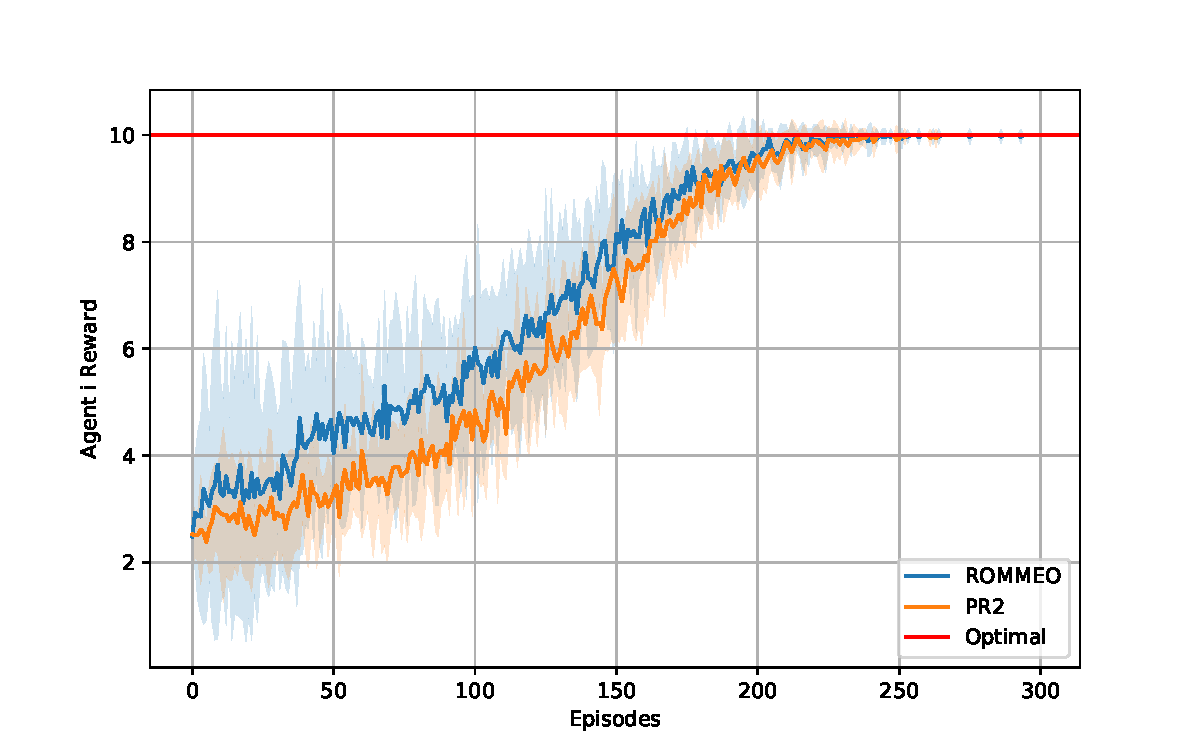
\includegraphics[scale=0.55]{figures/ROMMEO_PR2_ICG.pdf}
    \caption{The training progress of ROMMEO and PR2 on the cooperative game where the payoff is defined in equation \ref{eqn:chap3-matrix-game}.}
    \label{fig:chap3_ROMMEO_PR2}
\end{figure}
The reward of agent $j$ would be the same. We can see that ROMMEO does slightly better than PR2 as expected from the results presented in \cite{tian2019regularized}. We can see that due to the temperature schedule, the variances of both curves for the first 150 episodes are high, which is also a sign of exploration. Now, let's consider agent $i$ training when dealing with adversarial agent $j$ to study the impact of the variable $\beta^i$ and $\beta^j$ of agent $i$. We will follow the Balancing Q-learning algorithm, in which we have the following results shown in figure \ref{fig:chap3-comparison-balance-pr2-matrix}. First, in figure \ref{fig:chap3-balancing-q-min-max-matrix}, both agents converge to a Nash equilibrium when using Balancing Q-learning, which isn't the case for PR2. By misrepresentation of its opponent, agent $i$ trained under PR2 algorithm will choose action $3$ (since in cooperative case this is the best action) giving a lower reward of almost $0$ leading to suboptimal performance. On the other hand, agent $i$ that is trained under Balancing-Q will choose action $1$ yielding the reward of $2$, and reaches Nash equilibrium. 
\begin{figure}[h]
\centering
\begin{subfigure}{.5\textwidth}
  \centering
  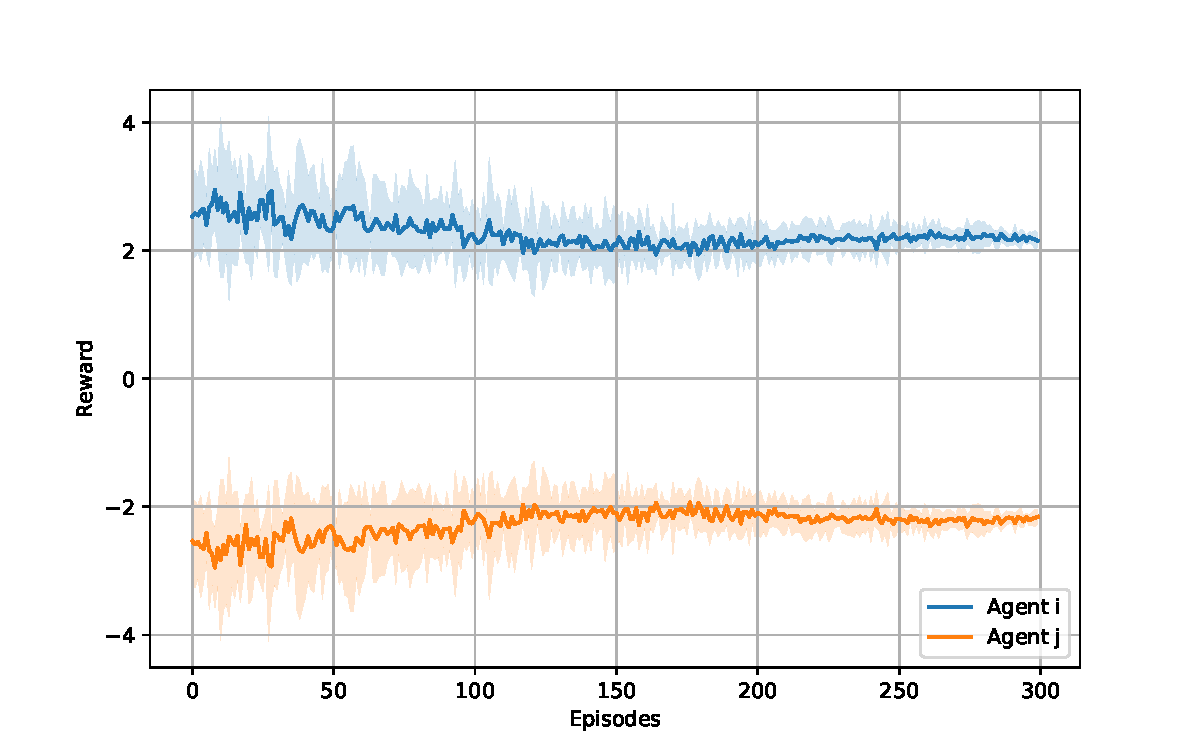
\includegraphics[width=\linewidth]{figures/Balancing_correct.pdf}
  \caption{Balancing Q-learning with adversarial opponent}
  \label{fig:chap3-balancing-q-min-max-matrix}
\end{subfigure}%
\begin{subfigure}{.5\textwidth}
  \centering
  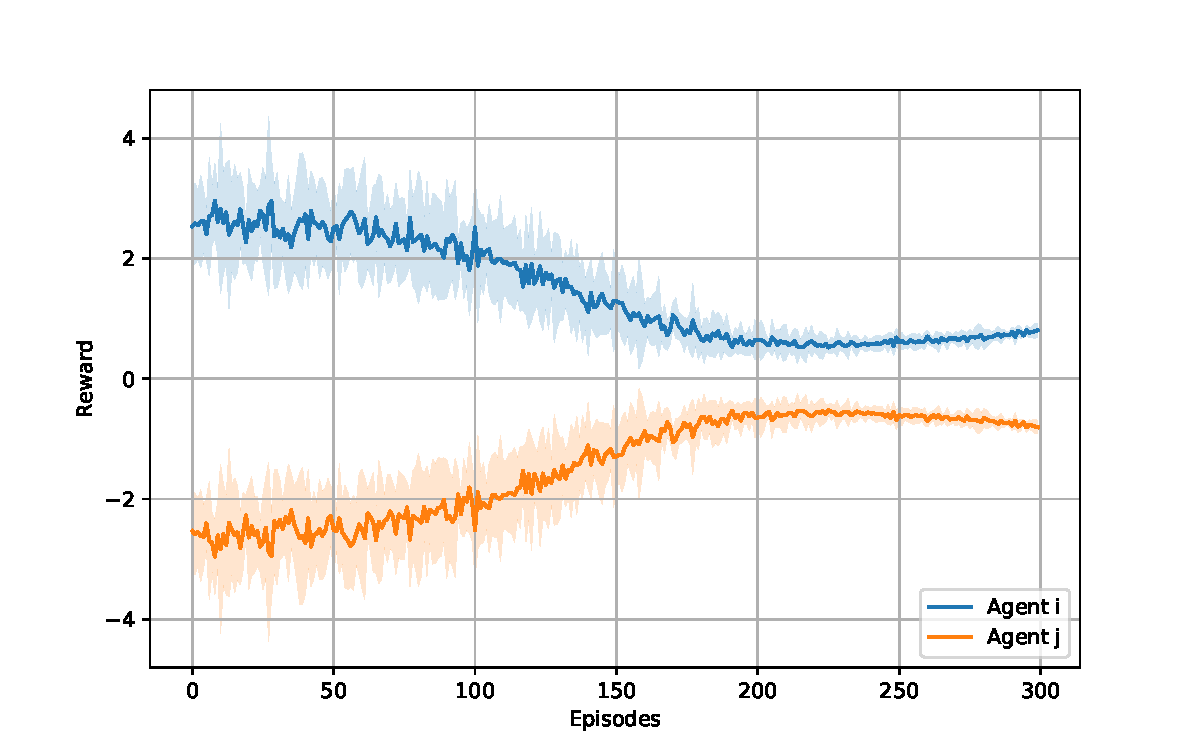
\includegraphics[width=\linewidth]{figures/Balancing_wrong.pdf}
  \caption{PR2 with misrepresentation of the opponent}
  \label{fig:chap3-pr2-min-max-matrix}
\end{subfigure}
\caption{A comparison between PR2 and Balancing Q-learning with adversarial opponent. PR2 can only represent cooperative opponent. Given the same set of seed the final reward are differ.}
\label{fig:chap3-comparison-balance-pr2-matrix}
\end{figure}

% Furthermore, one of the tricks that can be deployed to make the opponent model similar to the real opponent is to use supervised training on the prior opponent model given state and opponent action as a training set. By having a supervised opponent model, we can use it as a prior in our opponent model optimization as deployed in \cite{tian2019regularized}.

\subsection{What is Optimal ?}
We usually assume the optimality of the agent \textit{relative} to our knowledge of the opponent. If we are best responding to an optimal agent then we are likely to be optimal too\footnote{This is true in Nash equilibrium case by the definition.}. By jointly optimizing the agent with its opponent model, we can participate in what our opponent \textit{could be} given our assumptions and objective. This assumption is crucial, which will allow us to extend the framework so that it covers MAKL framework. We want to note that the assumption of an opponent's optimality is used in \cite{tian2019regularized}. However, it lacks the insight that the opponent's model doesn't have to follow the same objective as the agent, which we can show in the derivation of ROMMEO. In conclusion, MAPI is an enhanced probabilistic version of the fictitious play, where the opponent model is a fully trained policy. At the same time, the optimality of each agent should be independent while being based on each other, which is an inevitable contradiction but we will show that this is possible given special circumstances of Balancing Q-learning. 




\section{Derivation of ROMMEO}
Now, we shall consider the derivation of ROMMEO using the technique introduced in \cite{levine2018reinforcement}, which is shown briefly in section \ref{sec:chap2-derivation-soft-closed-form}. The working is partially covered in \cite{yu2019multi, wen2019multi} however a full derivation is required for the understanding of the algorithm. We will base our derivation for ROMMEO \cite{tian2019regularized}, while the same technique can be applied to PR2 \cite{wen2019probabilistic}. ROMMEO assumes that the joint probability between 2 agents, which can be factorized as
\begin{equation}
    \pi(a, a^{-i} | s) = \pi(a | a^{-i}, s) \rho(a^{-i} | s)
\end{equation}
factorizing in other ways yields PR2. We will start by drawing the graphical model of joint probabilities that we want to approximate, and is depicted in Figure \ref{fig:chap3-approximated-ROMMEO}. 
\begin{figure}[ht]
    \begin{minipage}[t]{0.5\linewidth}
    \centering
    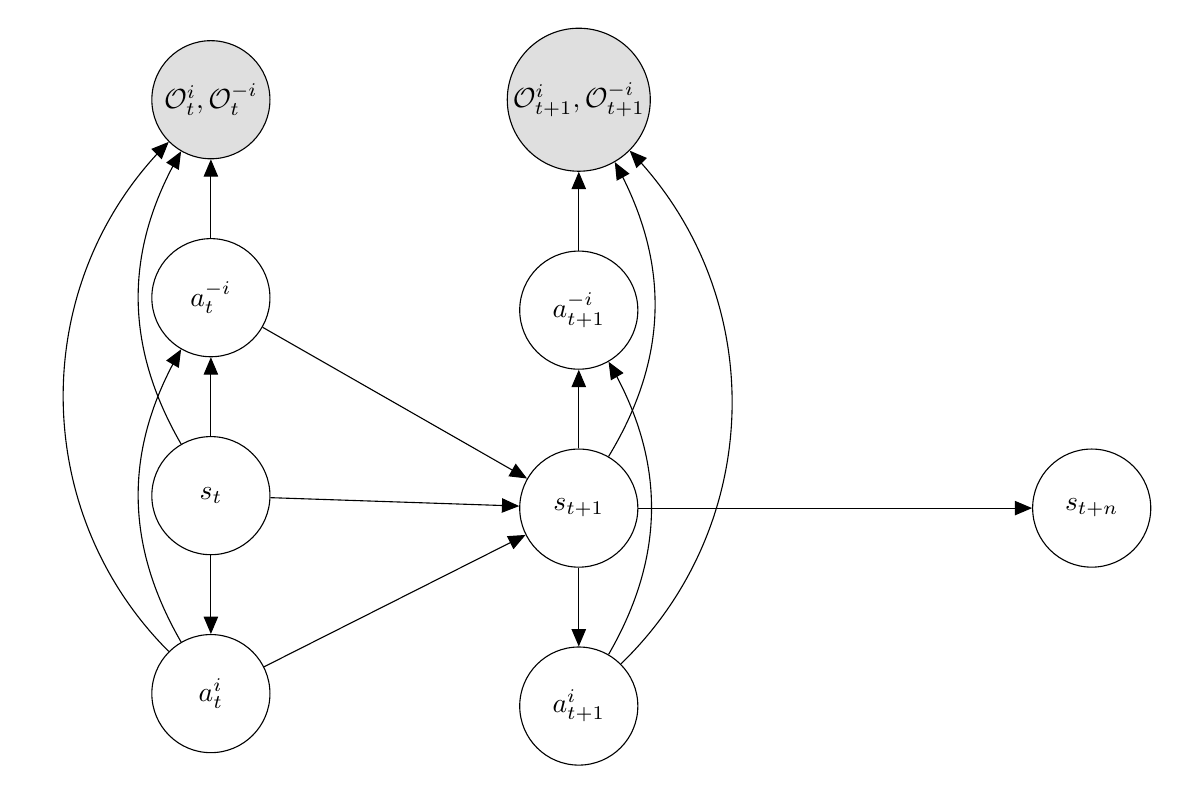
\begin{tikzpicture}[latent/.append style={minimum size=1.5cm}]
        \node[obs] (ot) {$\mathcal{O}^i_t, \mathcal{O}^{-i}_t$};
        \node[latent, below=of ot] (at) {$a^{-i}_t$};
        \node[latent, below=of at] (st) {$s_t$};
        \node[latent, below=of st] (a1t) {$a^i_t$};
        % \node[obs, below=of a1t] (o1t) {$\mathcal{O}^i_t$};
        
        
        % \path[->]  (o1)  edge   [bend left=45] node {} (a);
        % \edge{o1t} {a1t}
        \edge {st} {at, a1t}
        \edge {at} {ot}
        % \path[->]  (o1t)  edge   [bend left=60] node {} (ot);
        \path[->]  (a1t)  edge   [bend left=45] node {} (ot);
        \path[->]  (a1t)  edge   [bend left=30] node {} (at);
        \path[->]  (st)  edge   [bend left=30] node {} (ot);
        
        \node[obs, right=3cm of ot] (ot1) {$\mathcal{O}^i_{t+1}, \mathcal{O}^{-i}_{t+1}$};
        \node[latent, below=of ot1] (at1) {$a^{-i}_{t+1}$};
        \node[latent, below=of at1] (st1) {$s_{t+1}$};
        \node[latent, below=of st1] (a1t1) {$a^i_{t+1}$};
        % \node[obs, below=of a1t1] (o1t1) {$\mathcal{O}^i_{t+1}$};
        
        % \edge{o1t1} {a1t1}
        \edge {st1} {at1, a1t1}
        \edge {at1} {ot1}
        % \path[->]  (o1t1)  edge   [bend right=60] node {} (ot1);
        \path[->]  (a1t1)  edge   [bend right=45] node {} (ot1);
        \path[->]  (a1t1)  edge   [bend right=30] node {} (at1);
        \path[->]  (st1)  edge   [bend right=30] node {} (ot1);
        
        \path[->]  (st)  edge   [] node {} (st1);
        \path[->]  (at)  edge   [] node {} (st1);
        \path[->]  (a1t)  edge   [] node {} (st1);
        
        \node[latent, right=5cm of st1] (stn) {$s_{t+n}$};
        \path[->]  (st1)  edge [] node {} (stn);
    \end{tikzpicture}
    \end{minipage}%
    \begin{minipage}[t]{0.5\linewidth}
    \caption{Graphical model that we want to approximate. This is based on the joint probability provided in ROMMEO paper, with slight modification. The authors assume that the opponent we are playing against is optimal}
    \label{fig:chap3-approximated-ROMMEO}
    \end{minipage}
\end{figure}
Before we move on, please note that this is all within an agent calculation, while the opponent's policy will have the same process. Given this, we can show that the prior joint probability is equal to the following:
\begin{equation}
    \begin{aligned}
        P(s_{1:T}, &a^i_{1:T}, a^{-i}_{1:T}, \optim^{-i}_{1:T} = 1, \optim^{i}_{1:T} = 1) \\
        &= P(s_0) \prod^T_{t=0} P_{\prior}(a^i_t | s_t, a^{-i}_t) P_{\prior}(a^{-i}_t | s_t) P(s_{t+1} | s_t, a^i_t, a^{-i}_t) P(\optim^{-i}_t = 1, \optim^{i}_t = 1 | s_t, a^i_t, a^{-i}_t)
    \end{aligned}
\end{equation}
where the optimality variable is defined as 
\begin{equation}
\begin{aligned}
    &P(\optim_t^{-i} = 1, \optim^{i}_t = 1 | s_t, a^i_t, a^{-i}_t) \propto \exp \bracka{ \beta r(s_t, a^i_t, a^{-i}_t)  } \\
    &P(\optim_t^{-i} = 1, \optim^{i}_t = 1 | s_t, a^i_t, a^{-i}_t) = P(\optim_t^{-i} = 1 |\optim^{i}_t = 1, s_t, a^i_t, a^{-i}_t) P(\optim^{i}_t = 1 | \optim^{-i}_t = 1, s_t, a^i_t, a^{-i}_t)
\end{aligned}
\end{equation}
This definition is different from the one proposed in \cite{tian2019regularized}. However, we would like to point out that the opponent model has been optimized \textit{after} the agent's policy, which will show in a later section. Therefore, during the optimization of the opponent model, it has assumed that the agent's policy is optimal, hence the factorization of the optimality. Furthermore, the factorization of the optimality random variables above is a mere representation because the distinction between agent's and its opponent model lies during the calculation of the solution and not during the inference. Now for the variational joint probabilities that we want to optimize on the graphical model is depicted in Figure \ref{fig:chap3-variational-ROMMEO}.
\begin{figure}[ht]
    \begin{minipage}[t]{0.5\linewidth}
    \centering
    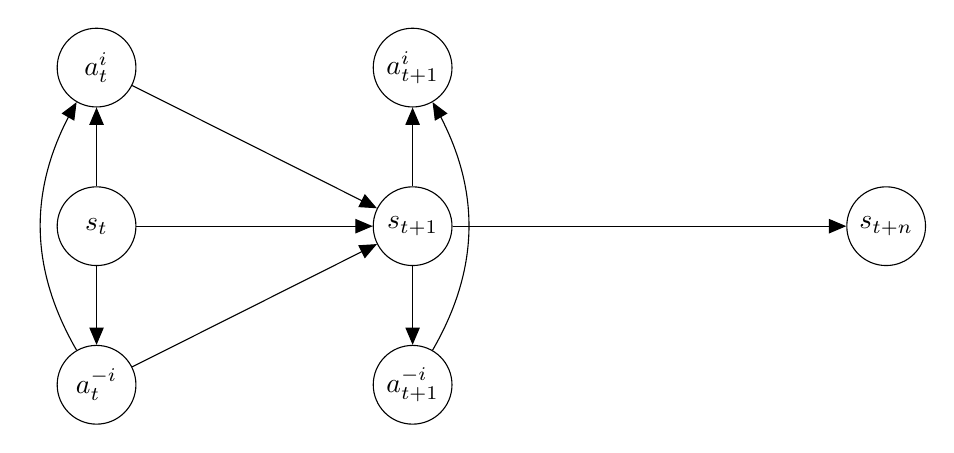
\begin{tikzpicture}[latent/.append style={minimum size=1.0cm}]
        \node[latent] (at) {$a^i_t$};
        \node[latent, below=of at] (st) {$s_t$};
        \node[latent, below=of st] (a1t) {$a^{-i}_t$};
        
        % \edge{o1t} {a1t}
        \edge {st} {at, a1t}
        % \edge {at} {ot}
        % \path[->]  (o1t)  edge   [bend left=60] node {} (ot);
        % \path[->]  (a1t)  edge   [bend left=45] node {} (ot);
        \path[->]  (a1t)  edge   [bend left=30] node {} (at);
        % \path[->]  (st)  edge   [bend left=30] node {} (ot);
        
        % \node[obs, right=3cm of ot] (ot1) {$\mathcal{O}^i_{t+1}$};
        \node[latent, right=3cm of at] (at1) {$a^i_{t+1}$};
        \node[latent, below=of at1] (st1) {$s_{t+1}$};
        \node[latent, below=of st1] (a1t1) {$a^{-i}_{t+1}$};
        % \node[obs, below=of a1t1] (o1t1) {$\mathcal{O}^{-i}_{t+1}$};
        
        % \edge{o1t1} {a1t1}
        \edge {st1} {at1, a1t1}
        % \edge {at1} {ot1}
        % \path[->]  (o1t1)  edge   [bend right=60] node {} (ot1);
        % \path[->]  (a1t1)  edge   [bend right=45] node {} (ot1);
        \path[->]  (a1t1)  edge   [bend right=30] node {} (at1);
        % \path[->]  (st1)  edge   [bend right=30] node {} (ot1);
        
        \path[->]  (st)  edge   [] node {} (st1);
        \path[->]  (at)  edge   [] node {} (st1);
        \path[->]  (a1t)  edge   [] node {} (st1);
        
        \node[latent, right=5cm of st1] (stn) {$s_{t+n}$};
        \path[->]  (st1)  edge [] node {} (stn);
    \end{tikzpicture}
    \end{minipage}%
    \begin{minipage}[t]{0.5\linewidth}
    \caption{Graphical model that we are going to optimize our policies on. This has almost the same structure as the version that we want to approximate. However, we don't care about the optimality of the agent itself, as we want to approximate its policy (denote as $\pi$) and the its opponent model (denote as $\rho$)}
    \label{fig:chap3-variational-ROMMEO}
    \end{minipage}
\end{figure}
The joint probability of variational distribution can be calculated as following 
\begin{equation}
    q(s_{1:T}, a_{1:T}^i, a^{-i}_{1:T}) = P(s_0) \prod^T_{t=0} \pi_{\theta}(a^i_t | s_t, a^{-i}_t) \rho_{\phi}(a^{-i}_t | s_t) P(s_{t+1} | s_t, a^i_t, a^{-i}_t)P(\optim^{-i}_t = 1)
\end{equation}
We would like to solve the following optimization problem 
\begin{equation}
    \argmin{\pi, \phi \in \Pi \times \Phi}  \kl\bracka{q(s_{1:T}, a_{1:T}^i, a^{-i}_{1:T}) \Big\| P(s_{1:T}, a^i_{1:T}, a^{-i}_{1:T}|\optim^i_{1:T} = 1  \optim^{-i}_{1:T} = 1) }
\end{equation}
This leads to optimizing the following ELBO. The derivation is shown in the appendix \ref{appx:chap3-ROMMEO-ELBO}, which translates the problem into a maximization problem of the following objective
\begin{equation}
\label{eqn:chap3-ROMMEO-ELBO}
    \argmax{\pi, \phi \in \Pi \times \Phi} \mathbb{E}_{q}\brackb{ \sum^T_{t=0} \gamma^t\bracka{\beta r(s_t, a^i_t, a^{-i}_t)  - \log \frac{\pi_{\theta}(a^i_t | s_t, a^{-i}_t)}{P_{\prior}(a^i_t | s_t, a^{-i}_t) } - \log \frac{\rho_{\phi}(a^{-i}_t | s_t)}{P_{\prior}(a^{-i}_t | s_t)}}}
\end{equation}
We will start off by considering the last time step, as we will progress backwards in time. Considering the last time step:
\begin{equation}
\label{eqn:training-obj-last-time}
    \mathbb{E}_{q} \brackb{ \beta r(s_T, a^i_T, a^{-i}_T)  - \log \frac{\pi_{\theta}(a^i_T | s_T, a^{-i}_T)}{P_{\prior}(a^i_T | s_T, a^{-i}_T) } - \log \frac{\rho_{\phi}(a^{-i}_T | s_T)}{P_{\prior}(a^{-i}_T | s_T)}}
\end{equation}
We can show that the optimal policy is equal to 
\begin{equation}
\begin{aligned}
    &\pi_{\theta}(a^i_T | s_T, a^{-i}_T) = \frac{\exp \bracka{\beta r(s_t, a^i_T, a^{-i}_T)}P_{\prior}(a^i_T | s_T, a^{-i}_T)}{\exp\bracka{Q(s_T, a^{-i}_T)}} \\
    \text{where }& Q(s_T, a^{-i}_T) = \log \int \exp \bracka{\beta R(s_T, a^i_T, a^{-i}_T}P_{\prior}(a^i_T | s_T, a^{-i}_T)  \dby a^i_T
\end{aligned}
\end{equation}
The proof will be presented in the appendix \ref{appx:chap3-ROMMEO-agent-last-time}. This part is where we can assume that the agent policy is optimal and allow us to calculate the opponent model objective. By plugging the optimal policy back, we are left with the opponent's objective:
\begin{equation}
    \mathbb{E}_{ \rho_{\phi}(a^{-i}_T | s_T) P(s_T)}\brackb{ Q(s_T, a^{-i}_T) - \log \frac{\rho_{\phi}(a^{-i}_T | s_T)}{P_{\prior}(a^{-i}_T | s_T)} }
\end{equation}
which will give us the optimal opponent model at time step $T$ to be as the following:
\begin{equation}
\begin{aligned}
    &\rho_{\phi}(a^{-i}_T | s_T)  = \frac{ \exp\bracka{Q(s_T, a^{-i}_T)}P_{\prior}(a^{-i}_T | s_T) }{\exp\bracka{V(s_T)}}  \\
    \text{where }& V(s_T) = \log \int \exp\bracka{Q(s_T, a^{-i}_T)}P_{\prior}(a^{-i}_T | s_T) \dby a^{-i}_T
\end{aligned}
\end{equation}
All the proofs including the opponent's objective is in appendix \ref{appx:chap3-ROMMEO-opponent-last-time}. Given both agent and its opponent's model policy, we can consider the message passed to the time steps before, and we can see that we are left with
\begin{equation}
    \mathbb{E}_{P(s_T)}\brackb{V(s_T)}
\end{equation}
This quantity will be passed down to the later time. Now for time $t$, the objective that we are optimizing becomes 
\begin{equation}
    \mathbb{E}_{q} \Bigg[ \underbrace{\beta r(s_t, a^i_T, a^{-i}_T) + \gamma \mathbb{E}_{P(s_{t+1} | s_t, a^i_t, a^{-i}_t)}  \brackb{V(s_{t+1})}}_{Q(s_t, a^i_t, a^{-i}_t)}  - \log \frac{\pi_{\theta}(a^i_T | s_t, a^{-i}_t)}{P_{\prior}(a^i_t | s_t, a^{-i}_t) } - \log \frac{\rho_{\phi}(a^{-i}_t | s_t)}{P_{\prior}(a^{-i}_t | s_t)} \Bigg]
\end{equation}
We can see that this leads to very similar problem as the one we have solved before. Therefore, by using the same proving process, we can derive the optimal agent's policy and optimal opponent model policy to be 
\begin{equation}
\begin{aligned}
    \label{eqn:chap3-final-ROMMEO-policy}
    \pi_{\theta}(a^i_t | s_t, a^{-i}_t) = \frac{\exp \bracka{Q(s_t, a^i_t, a^{-i}_t)}P_{\prior}(a^i_t | s_t, a^{-i}_t) }{\exp\bracka{Q(s_t, a^{-i}_t)}} \quad \quad \rho_{\phi}(a^{-i}_t | s_t) = \frac{ \exp\bracka{Q(s_t, a^{-i}_t)}P_{\prior}(a^{-i}_t | s_t) }{\exp\bracka{V(s_t)}}
\end{aligned}
\end{equation}
where the analogous "Bellman equation" is the following (with the value and action value functions being)
\begin{equation}
    \label{eqn:chap3-final-ROMMEO}
    \begin{aligned}
        &Q(s_t, a^i_t, a^{-i}_t) = \beta r(s_t, a^i_t, a^{-i}_t) + \gamma\mathbb{E}_{P(s_{t+1} | s_t, a^i_t, a^{-i}_t)} \brackb{V(s_{t+1})} \\
        \text{where }&Q(s_t, a^{-i}_t) = \log \int \exp \bracka{Q(s_t, a^i_t, a^{-i}_t}P_{\prior}(a^i_t | s_t, a^{-i}_t)  \dby a^i_t \\ 
        &V(s_t) = \log \int \exp\bracka{Q(s_t, a^{-i}_t)}P_{\prior}(a^{-i}_t | s_t) \dby a^{-i}_t \\
    \end{aligned}
\end{equation}    
This concludes the derivation for ROMMEO in its most general form. If we consider PR2, then we have to maximize opponent model first, by using a similar process.



\section{Interpretation of ROMMEO}
\label{sec:chap3-ROMMEO-interpretation}

\subsection{Understanding ROMMEO}
Before we examine the results, let's state some of the theoretical results for ROMMEO, which are discussed in \cite{tian2019regularized}. The authors showed that the Bellman equation in equation \ref{eqn:chap3-final-ROMMEO} is a contraction mapping, which shows that there exists a fixed point of agent and its opponent model action value function, while the updating agent and its opponent model does improve the action value. These results are analogous to results from section \ref{sec:chap2-derivation-soft-closed-form}. Thus ROMMEO is implemented via soft Actor-Critic like algorithm, see section \ref{sec:chap2-soft-ac-implement} and \cite{tian2019regularized} for more details. 

Let's examine the results that we get from the derivation of ROMMEO. We start with the definition of value function $V(s)$. Let's expand the meaning of it:
\begin{equation}
    V(s_{t}) =\mathbb{E}_{\pi_\theta, \rho_\phi}\brackb{Q(s_t, a^i_t, a^{-i}_t) - \log\frac{\rho_\phi(a^{-i}_t | s_t)}{P_\prior(a^{-i}_t | s_t)} - \log\frac{\pi_{\theta}(a^i_t | s_t, a^{-i}_t) }{P_{\prior}(a^i_t | s_t, a^{-i}_t)}}
\end{equation}
We can see that the Bellman equation holds for the following:
\begin{equation}
\begin{aligned}
\label{eqn:chap3-rollout-Q}
    Q(s_{t},& a^i_{t}, a^{-i}_{t}) = \beta r(s_t, a^i_t, a^{-i}_t) \\
    &+ \gamma\mathbb{E}_{s_{t+1}}\brackb{\mathbb{E}_{\pi_\theta, \rho_\phi}\brackb{Q(s_{t+1}, a^i_{t+1}, a^{-i}_{t+1}) - \log\frac{\rho_\phi(a^{-i}_{t+1} | s_{t+1})}{P_\prior(a^{-i}_{t+1} | s_{t+1})} - \log\frac{\pi_{\theta}(a^i_{t+1} | s_{t+1}, a^{-i}_{t+1}) }{P_{\prior}(a^i_{t+1} | s_{t+1}, a^{-i}_{t+1})}}}
\end{aligned}
\end{equation}
Please keep in mind that for the value function to be complete, we have to consider the regularizers for both policy and its opponent model, which is equivalent to the use of soft-max on action-value function, when we use the optional policies. Furthermore, the exciting part is how the agent's policy uses this function. Since we have expanded the equation, we can see that the value function is based on the expectation of \correctquote{optimal} opponent model\footnote{during training we don't have the exact form due to approximation error}, which means that the agent is also considering the optimality of opponent model implicitly. By reaching the fixed point\footnote{We don't think that it is the same as logistic stochastic best response equilibrium (LSBRE) that is proposed in \cite{yu2019multi} because we don't refer to any stationary distribution of any Markov chain. But they should be related somehow, and we left it for future work.}, we perfectly capture how the agent considers its opponent model to be optimal and how the opponent model considers an optimal agent, which can't be described probabilistically. One might wonder how does the agent $\pi_\theta(a^i_t | s_t, a^{-i}_t)$ executes its action ? According to \cite{tian2019regularized}, we can simply plug the value of opponent models so that the agent can return the action as we assume the optimality of the opponent model onward i.e 
\begin{equation}
\label{eqn:chap3-ROMMEO-execute-action}
\pi_\theta(a^i_t |s_t) = \int \pi_\theta(a^i_t | s_t, a^{-i}_t) \rho_\phi(a^{-i}_t | s_t) \dby a^{-i}_t 
\end{equation}
However, please note that the agent is best responding to its opponent model only and not the opponent itself (see the rollout or even ELBO in equation \ref{eqn:chap3-rollout-Q} and \ref{eqn:chap3-ROMMEO-ELBO} relatively). This might be trivial, but it can be a very subtle thing to miss. Let's view the value function from other forms, starting with the action-value function 
\begin{equation}
    Q(s_t, a^{-i}_t) = \log \int \exp \bracka{Q(s_t, a^i_t, a^{-i}_t}P_{\prior}(a^i_t | s_t, a^{-i}_t)  \dby a^i_t 
    % &V(s_t) = \log \int \exp\bracka{Q(s_t, a^{-i}_t)}P_{\prior}(a^{-i}_t | s_t) \dby a^{-i}_t
\end{equation}
This represents the action-value function for the opponent model as it only contains the state and opponent model's action. As mentioned before\footnote{in section \ref{sec:chap2-derivation-soft-closed-form}}, this resembles \correctquote{soft-max} of agent's action based on agent's prior. In other words, the opponent model's action-value function is the maximization of full action-value function that is also influenced by the opponent's\footnote{or opponent model i.e agent's belief that opponent will use $P_\prior (a^i_t | s_t, a^{-i}_t)$ as its (refer to opponent) prior for the agent} prior on agent policy. The opponent models doesn't simply use an expected value of the action value given agent's prior i.e $\mathbb{E}_{P_\prior (a^i_t | s_t, a^{-i}_t)}\brackb{Q(s_t, a^i_t, a^{-i}_t)}$ nor uses the action that maximizes agent's value i,e $\max_{a^i_t} Q(s_t, a^i_t, a^{-i}_t)$, but a mixture of both - prior based best response, since we know that the agent will try to increase its expected reward (a maximize) while trying to acts similarly to its prior (expected value). This is crucial, since the prior is not only a regularizer for the agent, but it also represents the opponent's belief on what the agent should do. In conclusion, MAPI framework doesn't only best response to the opponent model that is estimated via supervised learning but also best responding to optimal opponent the agent aware of.



\section{Solving Balancing-Q learning}
\label{sec:chap3-balancing-Q}

\subsection{Policies Derivation}
\label{sec:chap3-balancing-Q-derivation}
Instead of having a ELBO that we want to maximize, we initially have the following loss function from \cite{grau2018balancing}:
\begin{equation}
    \mathbb{E}_q\left[ \sum^T_{t=0} \gamma^t \bracka{r(s_t, a_t, a^{-i}_t) - \frac{1}{\beta^i} \log\frac{\pi_{\theta}(a_t|s_t)}{P_\prior(a^i_t|s_t)} - \frac{1}{\beta^{-i}}\log \frac{\rho_\phi(a^{-i}_t|s_t)}{P_\prior(a^{-i}_t|s_t)}} \right]
\end{equation}
However, as noted in section before that by using our familiar method, we should consider the conditional opponent model $\rho_\phi(a^{-i}_t | s_t, a^i_t)$ in order to arrive at the final optimal policy. In \cite{grau2018balancing} the authors doesn't explicitly show us the method of solving, we, therefore, are going to proposed one of the ways, the derivation can be done. Note that the loss function above assume no opponent model. However, to turn closer to MAPI approach, we shall consider similar formulation as PR2 \cite{wen2019probabilistic} case i.e 
\begin{equation}
    \mathbb{E}_q\left[ \sum^T_{t=0} \gamma^t \bracka{r(s_t, a_t, a^{-i}_t) - \frac{1}{\beta^i} \log\frac{\pi_{\theta}(a_t|s_t)}{P_\prior(a^i_t|s_t)} - \frac{1}{\beta^{-i}}\log \frac{\rho_\phi(a^{-i}_t | s_t, a^i_t)}{P_\prior(a^{-i}_t | s_t, a^i_t)}} \right]
\end{equation}
Now, it is an objective that is optimized within the agent and doesn't required any opponent. We will see that this leads to the same final optimal policy fir the agent. Starting with the final time step we have:
\begin{equation}
    \mathbb{E}_{P(s_T) P(a_T, a^{-i}_T | s_T)}\left[ r(s_t, a_t, a^{-i}_t) - \frac{1}{\beta^i} \log\frac{\pi_{\theta}(a^i_T|s_T)}{P_\prior(a^i_T|s_T)} - \frac{1}{\beta^{-i}}\log \frac{\rho_\phi(a^{-i}_T|s_T, a^i_T)}{P_\prior(a^{-i}_T|s_T, a^i_T)} \right]
\end{equation}
Using the rearrangement and minimizing KL-divergence, we can show that
\begin{equation}
\begin{aligned}
    &\rho(a^{-i}_T | s_T, a^i_T) = \frac{ \exp\bracka{\beta^{-i} r(s_t, a_t, a^{-i}_t)} P_{\prior}(a^{-i}_T|s_T, a^i_T)}{\exp\bracka{Q^{-i}(s_T, a^{i}_T)}}\\
    \text{where }& Q^{-i}(s_T, a^{i}_T) = \log \int \exp\bracka{\beta^{-i} r(s_t, a_t, a^{-i}_t)} P_{\prior}(a^{-i}_T|s_T, a^i_T) \dby a^{-i}
\end{aligned}
\end{equation}
see appendix \ref{appx:chap4-balancing-q-oppo-model} for full derivation. Now consider the message left by plugging the agent's policy back\footnote{we want to make sure that we got correct action value since we have multiple $\beta$s finding the right value can be confusing.}, which leads to the following agent's objective:
\begin{equation}
    \mathbb{E}_{P(s_T, a_T, a^{-i}_T)}\bigg[ \underbrace{\frac{\beta^i}{\beta^{-i}} Q^{-i}(s_T, a^{i}_T)}_{Q^i(s_T, a^{i}_T)} - \log\frac{\pi_{\theta}(a^i_T|s_T)}{P_\prior(a^i_T|s_T)}\bigg]
\end{equation}
Given this, we can consider the agent's optimal policy, which is equal to 
\begin{equation}
\begin{aligned}
    &\pi_{\theta}(a^i_T|s_T) = \frac{ \exp\bracka{Q^i(s_T, a^{i}_T)}P_\prior(a^i_T|s_T)} {\exp\bracka{V^i(s_T)}} \\
    \text{where }& Q^i(s_T, a^{i}_T) = \frac{\beta^i}{\beta^{-i}} \log \int \exp\bracka{\beta^{-i} R(s_T, a^i_T, a^{-i}_T)} P_{\prior}(a^{-i}_T|s_T) \dby a^{-i} \\
    \text{and }& V^i(s_T) = \log \int  \exp\bracka{Q^i(s_T, a^{i}_T)}P_\prior(a^i_T|s_T) \dby a^i
\end{aligned}
\end{equation}
See appendix for full derivation of both agent's objective optimal agent's policy, while we are left with the following message:
\begin{equation}
    \mathbb{E}_{P(s_T)}\brackb{\frac{1}{\beta^i}V^i(s_T)} = \mathbb{E}_{P(s_T)}\brackb{V(s_T)}
\end{equation}
Let's consider the arbitrary time step $t$, which lead us to the following objective 
\begin{equation}
    \mathbb{E}_{P(s_t, a_t, a^{-i}_t)}\Bigg[ \underbrace{r(s_t, a_t, a^{-i}_t) + \gamma\mathbb{E}_{P(s_{t+1} | s_t, a_t, a^{-i}_t)}\brackb{V(s)}}_{Q(s_t, a^i_t, a^{-i}_t)} - \frac{1}{\beta^i} \log\frac{\pi_{\theta}(a_t|s_t)}{P_\prior(a^i_t|s_t)} - \frac{1}{\beta^{-i}}\log \frac{\rho_\phi(a^{-i}_t | s_t, a^i_t)}{P_\prior(a^{-i}_t | s_t, a^i_t)} \Bigg]
\end{equation}
By solving using the same method, we have the following optimal agent's policy
\begin{equation}
\begin{aligned}
    &\pi_{\theta}(a^i_t|s_t) = \frac{ \exp\bracka{Q^i(s_t, a^{i}_t)}P_\prior(a^i_t|s_t)} {\exp\bracka{V^i(s_t)}} \\
    \text{ where }
    &Q^{i}(s_t, a^{i}_t) = \frac{\beta^i}{\beta^{-i}} \log \int \exp\bracka{\beta^{-i} Q(s_t, a^i_t, a^{-i}_t)} P_{\prior}(a^{-i}_t|s_t) \dby a^{-i} \\
    &V^{i}(s_t) = \log \int  \exp\bracka{Q^i(s_t, a^{i}_t)}P_\prior(a^i_t|s_t) \dby a^i\\
\end{aligned}
\end{equation}
For the definition of $Q(s_t, a^i_t, a^{-i}_t)$ will be define at the end, after consider the definition of optimal opponent agent, which is a solution to the following objective:
\begin{equation}
    \mathbb{E}_q\left[ \sum^T_{t=0} \gamma^t \bracka{r(s_t, a_t, a^{-i}_t) - \frac{1}{\beta^i} \log\frac{\pi_{\theta}(a_t|s_t, a^{-i}_t)}{P_\prior(a^i_t|s_t, a^{-i}_t)} - \frac{1}{\beta^{-i}}\log \frac{\rho_\phi(a^{-i}_t | s_t)}{P_\prior(a^{-i}_t | s_t)}} \right]
\end{equation}
which lead to the following results, using the same techniques as the derivation of policy:
\begin{equation}
\begin{aligned}
    &\rho_{\phi}(a^{-i}_t|s_t) = \frac{ \exp\bracka{Q^{-i}(s_t, a^{-i}_t)}P_\prior(a^{-i}_t|s_t)} {\exp\bracka{V^{-i}(s_t)}} \\
    \text{ where }&Q^{-i}(s_t, a^{-i}_t) = \frac{\beta^{-i}}{\beta^{i}} \log \int \exp\bracka{\beta^{i} Q(s_t, a^i_t, a^{-i}_t)} P_{\prior}(a^{i}_t|s_t, a^{-i}_t) \dby a^{i}  \\
    &V^{-i}(s_t) = \log \int \exp\bracka{Q^{-i}(s_t, a^{-i}_t)}P_\prior(a^{-i}_t|s_t) \dby a^{-i}  \\
\end{aligned}
\end{equation}
The authors \cite{grau2018balancing} proved that the value function of the agent and the opponent are related as follows:
\begin{equation}
\label{eqn:chap3-balance-value-equivalent}
    \gamma\mathbb{E}_{P(s_t)}\brackb{V(s)} = \gamma \mathbb{E}_{P(s_t)}\brackb{\frac{1}{\beta^i} V^i(s_t)} = \gamma\mathbb{E}_{P(s_t)}\brackb{\frac{1}{\beta^{-i}} V^{-i}(s_t)}
\end{equation}
We can, therefore, learn the same Q-value function:
\begin{equation}
    Q(s_t, a^i_t, a^{-i}_t) = r(s_t, a_t, a^{-i}_t) + \mathbb{E}_{P(s_{t+1} | s_t, a_t, a^{-i}_t)}\brackb{V(s_{t+1})}
\end{equation}
Intuitively, we can see that $\beta^i$ and $\beta^{-i}$ are canceling each others. This is very interesting as we can control how the opponent model learns while able to control \correctquote{correct} type of the game. This is, indeed, a special case as we can't usually control the opponent's reward to be as effective as this. 

\subsection{Theoretical Properties}
\label{sec:chap3-balancing-Q-theoretical}
Now, we shall consider the theoretical property of the algorithm. We start with the result from \cite{grau2018balancing}, where the authors show that Balancing Q-learning Bellman equation:
\begin{equation}
    \contractop_{\text{Balance}} Q(s_t, a^i_t, a^{-i}_t) = r(s_t, a_t, a^{-i}_t) + \mathbb{E}_{P(s_{t+1} | s_t, a_t, a^{-i}_t)}\brackb{V(s_{t+1})}
\end{equation}
is a contraction mapping. We would like to further investigate more on how the agent's update affects the action value function. Suppose a fixed policy $\pi$, how would an updated opponent affects the action value function given the value $\beta^{-i}$
\begin{theorem}
\label{thm:update-balance-opponent}
    The action value function $Q^{-i, \pi, \rho}(s_t, a^i_t, a^{-i}_t)$ defined by Bellman equation as:
    \begin{equation}
    \begin{aligned}
        Q^{-i, \pi, \rho}&(s_t, a^i_t, a^{-i}_t) = r(s_t, a_t, a^{-i}_t) \\
        &+ \gamma\mathbb{E}_{s_{t+1}}\brackb{\mathbb{E}_{\pi, \rho}\brackb{Q^{-i, \pi, \rho}(s_{t+1}, a^i_{t+1}, a^{-i}_{t+1}) - \frac{1}{\beta^i} \log\frac{\pi(a^i_{t+1}|s_{t+1}, a^{-i}_{t+1})}{P_\prior(a^i_{t+1}|s_{t+1}, a^{-i}_{t+1})} - \frac{1}{\beta^{-i}}\log \frac{\rho(a^{-i}_{t+1}|s_{t+1})}{P_\prior(a^{-i}_{t+1}|s_{t+1})}}}
    \end{aligned}
    \end{equation}
    Given the opponent's updated policy $\tilde{\rho}$ given normal policy $\rho$ as 
    \begin{equation}
    \begin{aligned}
        \tilde{\rho}(a^{-i}_t | s_t) &= \argmin{\rho' \in \Pi} \kl \bracka{ \rho'(a^{-i}_t | s_t) \Bigg\| \frac{\exp\bracka{Q^{-i, \pi, \rho}(s_t, a^{-i}_t)} P_\prior(a^{-i}_t | s_t)}{\exp Z^{-i, \pi, \rho}(s_t)}} \\
        &=\argmin{\rho' \in \Pi} J_{\rho}(\rho')
    \end{aligned}
    \end{equation}
    The action-value function is affected in difference way according to the sign of $\beta^{-i}$
    \begin{equation}
    \begin{cases}
        Q^{-i, \pi, \rho}(s_t, a^i_t, a^{-i}_t) \ge Q^{-i, \pi, \tilde{\rho}}(s_t, a^i_t, a^{-i}_t) &\text{ if } \beta^{-i} < 0 \\
        Q^{-i, \pi, \rho}(s_t, a^i_t, a^{-i}_t) \le Q^{-i, \pi, \tilde{\rho}}(s_t, a^i_t, a^{-i}_t)&\text{ if } \beta^{-i} > 0
    \end{cases}
    \end{equation}
\end{theorem}
\begin{proof}
The proof follows closely from ROMMEO proof on policy improvement \cite{tian2019regularized} which is based on soft Actor-Critic \cite{haarnoja2018softa} proof for more details on the method see appendix \ref{appx:chap2-soft-policy-update-improvement}. We start by comparing these 2 quantities:
\begin{equation*}
\begin{aligned}
    &\mathbb{E}_{\pi, \red{\rho}}\brackb{Q^{-i, \pi, \rho}(s_{t+1}, a^i_{t+1}, a^{-i}_{t+1}) - \frac{1}{\beta^i} \log\frac{\pi(a^i_{t+1}|s_{t+1}, a^{-i}_{t+1})}{P_\prior(a^i_{t+1}|s_{t+1}, a^{-i}_{t+1})} - \frac{1}{\beta^{-i}}\log \frac{\red{\rho}(a^{-i}_{t+1}|s_{t+1})}{P_\prior(a^{-i}_{t+1}|s_{t+1})}} \\
    &\mathbb{E}_{\pi, \red{\tilde{\rho}}}\brackb{Q^{-i, \pi, \rho}(s_{t+1}, a^i_{t+1}, a^{-i}_{t+1}) - \frac{1}{\beta^i} \log\frac{\pi(a^i_{t+1}|s_{t+1}, a^{-i}_{t+1})}{P_\prior(a^i_{t+1}|s_{t+1}, a^{-i}_{t+1})} - \frac{1}{\beta^{-i}}\log \frac{\red{\tilde{\rho}}(a^{-i}_{t+1}|s_{t+1})}{P_\prior(a^{-i}_{t+1}|s_{t+1})}}
\end{aligned}
\end{equation*}
The differences are shown in red letter. Please note that the action value function definition of the second equation still based on the old opponent $\rho$. We start by finding the KL-divergence between arbitrary $\rho^+$ the objective for updating is the following, which can be expanded as 
\begin{equation*}
\begin{aligned}
    &\kl \bracka{ \rho^+(a^{-i}_t | s_t) \Bigg\| \frac{\exp\bracka{Q^{-i, \pi, \rho}(s_t, a^{-i}_t)} P_\prior(a^{-i}_t | s_t)}{\exp Z^{-i, \pi, \rho}(s_t)}} \\
    &= \int  \rho^+(a^{-i}_{t+1} | s_{t+1}) \log \frac{\rho^+(a^{-i}_{t+1} | s_{t+1}) \exp(Z^{-i, \pi, \rho}(s_{t+1})) }{P_\prior(a^{-i}_{t+1} | s_{t+1}) \exp\bracka{Q^{-i, \pi, \rho}(s_{t+1}, a^{-i}_{t+1})} } \dby a^{-i}_{t+1} \\
    &=\begin{aligned}[t]
    \int &\rho^+(a^{-i}_{t+1} | s_{t+1}) \log\frac{\rho^+(a^{-i}_{t+1} | s_{t+1})}{P_\prior(a^{-i}_{t+1} | s_{t+1})} \dby a^{-i}_{t+1} + Z^{-i, \pi, \rho}(s_{t+1}) \\
    &- \int \rho^+(a^{-i}_{t+1} | s_{t+1}) Q^{-i, \pi, \rho}(s_{t+1}, a^{-i}_{t+1}) \dby a^{i}_{t+1}
    \end{aligned}
\end{aligned}
\end{equation*}
Now the performance gap can be established due to the KL-divergence between $\rho$ and $\tilde{\rho}$. Please note that by definition $J_{\rho}(\rho) \ge J_{\rho}(\tilde{\rho})$ which leads to the following inequality
\begin{equation*}
\begin{aligned}
&\begin{aligned}[t]
    \int &\rho(a^{-i}_{t+1} | s_{t+1}) \log\frac{\rho(a^{-i}_{t+1} | s_{t+1})}{P_\prior(a^{-i}_{t+1} | s_{t+1})} \dby a^{-i}_{t+1} + \cancel{Z^{-i, \pi, \rho}(s_{t+1})} \\
    &- \int \rho(a^{-i}_{t+1} | s_{t+1}) Q^{-i, \pi, \rho}(s_{t+1}, a^{-i}_{t+1}) \dby a^{i}_{t+1}
\end{aligned} \\
\ge&\begin{aligned}[t]
    \int &\tilde{\rho}(a^{-i}_{t+1} | s_{t+1}) \log\frac{\tilde{\rho}(a^{-i}_{t+1} | s_{t+1})}{P_\prior(a^{-i}_{t+1} | s_{t+1})} \dby a^{-i}_{t+1} + \cancel{Z^{-i, \pi, \rho}(s_{t+1})} \\
    &- \int \tilde{\rho}(a^{-i}_{t+1} | s_{t+1}) Q^{-i, \pi, \rho}(s_{t+1}, a^{-i}_{t+1}) \dby a^{i}_{t+1}
\end{aligned}
\end{aligned}
\end{equation*}
Let's investigate more into the definition of the last term, for $\tilde{\rho}$. We will have to consider the opponent model of the agent
\begin{equation}
    \int \tilde{\rho}(a^{-i}_{t+1} | s_{t+1}) \frac{\beta^{-i}}{\beta^{i}} \bracka{\beta^iQ(s_t, a^i_t, a^{-i}_t) - \log \frac{\pi(a^i_t | a^{-i}_t, s_t)}{P_\prior(a^i_t | s_t)}} \dby a^{-i}_{t+1}
\end{equation}
which has the following definition of opponent's agent model:
\begin{equation*}
    \pi(a^i_t | a^{-i}_t, s_t) = \frac{\exp(\beta^i Q^{-i, \pi, \rho}(s_t, a^i_t, a^{-i}_t)) P_\prior(a^i_t | s_t)}{\exp\bracka{Q^{i, \pi, \rho}(s_t, a^{-i}_t)}}
\end{equation*}
We expand the definition to be:
\begin{equation*}
\begin{aligned}
    &\int \tilde{\rho}(a^{-i}_{t+1} | s_{t+1}) Q^{-i, \pi, \rho}(s_{t+1}, a^{-i}_{t+1}) \dby a^{-i}_{t+1} \\
    =& \int \rho(a^{-i}_{t+1} | s_{t+1}) \int \pi(a^i_{t+1} | a^{-i}_{t+1}, s_{t+1}) \brackb{\beta^{-i}Q(s_{t+1}, a^i_{t+1}, a^{-i}_{t+1}) - \frac{\beta^{-i}}{\beta^{i}}\log \frac{\pi(a^i_{t+1} | a^{-i}_{t+1}, s_{t+1})}{P_\prior(a^i_{t+1} | s_{t+1})}} \dby a^{i}_{t+1} \dby a^{-i}_{t+1} \\
    =& \mathbb{E}_{a^i_{t+1}, a^{-i}_{t+1} \sim \pi, \tilde{\rho}} \brackb{\beta^{-i}Q(s_{t+1}, a^i_{t+1}, a^{-i}_{t+1}) - \frac{\beta^{-i}}{\beta^i} \mathbb{E}_{a^i_{t+1}}\log \frac{\pi(a^i_{t+1} | a^{-i}_{t+1}, s_{t+1})}{P_\prior(a^i_{t+1} | s_{t+1})}}
\end{aligned}
\end{equation*}
Plugging this back into the equation, which some arrangement, we have 
\begin{equation*}
\begin{aligned}
&\begin{aligned}[t]
    \mathbb{E}_{a^i_{t+1}, a^{-i}_{t+1} \sim \pi, \rho}\Bigg[\beta^{-i}Q(s_{t+1}, a^i_{t+1}, a^{-i}_{t+1}) - \log\frac{\rho(a^{-i}_{t+1} | s_{t+1})}{P_\prior(a^{-i}_{t+1} | s_{t+1})} - \frac{\beta^{-i}}{\beta^i} \mathbb{E}_{a^i_{t+1}}\log \frac{\pi(a^i_{t+1} | a^{-i}_{t+1}, s_{t+1})}{P_\prior(a^i_{t+1} | s_{t+1})}\Bigg]
\end{aligned} \\
\le&\begin{aligned}[t]
    &\mathbb{E}_{a^i_{t+1}, a^{-i}_{t+1} \sim \pi, \tilde{\rho}}\Bigg[\beta^{-i}Q(s_{t+1}, a^i_{t+1}, a^{-i}_{t+1}) -\log\frac{\tilde{\rho}(a^{-i}_{t+1} | s_{t+1})}{P_\prior(a^{-i}_{t+1} | s_{t+1})} - \frac{\beta^{-i}}{\beta^i} \mathbb{E}_{a^i_{t+1}}\log \frac{\pi(a^i_{t+1} | a^{-i}_{t+1}, s_{t+1})}{P_\prior(a^i_{t+1} | s_{t+1})}\Bigg]
\end{aligned}
\end{aligned}
\end{equation*}
In the case that $\beta^{-i} < 0$, we have the following inequality:
\begin{equation*}
\begin{aligned}
    &\mathbb{E}_{a^i_{t+1}, a^{-i}_{t+1} \sim \rho}\bigg[-\frac{1}{\beta^i}\log \frac{\pi(a^i_{t+1} | s_{t+1}, a^{-i}_{t+1})}{P_\prior(a^i_{t+1} | s_{t+1}, a^{-i}_{t+1})} - \frac{1}{\beta^{-i}}\log \frac{\rho(a^{-i}_{t+1} | s_{t+1})}{P_\prior(a^{-i}_{t+1} | s_{t+1})} + Q^{-i, \pi, \rho}(s_{t+1}, a^i_{t+1}, a^{-i}_{t+1}) \bigg] \\
    \ge &\mathbb{E}_{a^i_{t+1}, a^{-i}_{t+1} \sim \tilde{\rho}}\bigg[-\frac{1}{\beta^i}\log \frac{\pi(a^i_{t+1} | s_{t+1}, a^{-i}_{t+1})}{P_\prior(a^i_{t+1} | s_{t+1}, a^{-i}_{t+1})} - \frac{1}{\beta^{-i}}\log \frac{\tilde{\rho}(a^{-i}_{t+1} | s_{t+1})}{P_\prior(a^{-i}_{t+1} | s_{t+1})} + Q^{-i, \pi, \rho}(s_{t+1}, a^i_{t+1}, a^{-i}_{t+1}) \bigg]
\end{aligned}
\end{equation*}
Now, let's consider the  recursive definition of action value function $Q^{-i, \pi, \rho}(s_{t+1}, a^i_{t+1}, a^{-i}_{t+1})$, which leads to the fact that 
\begin{equation}
    Q^{-i, \pi, \rho}(s_{t+1}, a^i_{t+1}, a^{-i}_{t+1}) \ge Q^{-i, \pi, \tilde{\rho}}(s_{t+1}, a^i_{t+1}, a^{-i}_{t+1})
\end{equation}
The recursive step will be shown in appendix \ref{appx:chap4-balancing-q-recrusive-Q} due to space constrain. Similarly, $\beta^{-i} > 0$, we have the inequality:
\begin{equation*}
\begin{aligned}
    &\mathbb{E}_{a^i_{t+1}, a^{-i}_{t+1} \sim \rho}\bigg[-\frac{1}{\beta^i}\log \frac{\pi(a^i_{t+1} | s_{t+1}, a^{-i}_{t+1})}{P_\prior(a^i_{t+1} | s_{t+1}, a^{-i}_{t+1})} - \frac{1}{\beta^{-i}}\log \frac{\rho(a^{-i}_{t+1} | s_{t+1})}{P_\prior(a^{-i}_{t+1} | s_{t+1})} + Q^{-i, \pi, \rho}(s_{t+1}, a^i_{t+1}, a^{-i}_{t+1}) \bigg] \\
    \le &\mathbb{E}_{a^i_{t+1}, a^{-i}_{t+1} \sim \tilde{\rho}}\bigg[-\frac{1}{\beta^i}\log \frac{\pi(a^i_{t+1} | s_{t+1}, a^{-i}_{t+1})}{P_\prior(a^i_{t+1} | s_{t+1}, a^{-i}_{t+1})} - \frac{1}{\beta^{-i}}\log \frac{\tilde{\rho}(a^{-i}_{t+1} | s_{t+1})}{P_\prior(a^{-i}_{t+1} | s_{t+1})} + Q^{-i, \pi, \rho}(s_{t+1}, a^i_{t+1}, a^{-i}_{t+1}) \bigg]
\end{aligned}
\end{equation*}
this leads to $Q^{-i, \pi, \rho}(s_{t+1}, a^i_{t+1}, a^{-i}_{t+1}) \le Q^{-i, \pi, \tilde{\rho}}(s_{t+1}, a^i_{t+1}, a^{-i}_{t+1})$. We have proven the way $\beta^{-i}$ affects the update of opponent policy.
\end{proof}
Similarly, we can show for the policy that 
\begin{theorem}
\label{thm:update-balance-agent}
    The action value function $Q^{i, \pi, \rho}(s_t, a^i_t, a^{-i}_t)$ defined by Bellman equation as:
    \begin{equation}
    \begin{aligned}
        Q^{i, \pi, \rho}&(s_t, a^i_t, a^{-i}_t) = r(s_t, a_t, a^{-i}_t) \\
        &+ \gamma\mathbb{E}_{s_{t+1}}\brackb{\mathbb{E}_{\pi, \rho}\brackb{Q^{i, \pi, \rho}(s_{t+1}, a^i_{t+1}, a^{-i}_{t+1}) - \frac{1}{\beta^i} \log\frac{\pi(a^i_{t+1}|s_{t+1})}{P_\prior(a^i_{t+1}|s_{t+1})} - \frac{1}{\beta^{-i}}\log \frac{\rho(a^{-i}_{t+1}|s_{t+1}, a^i_{t+1})}{P_\prior(a^{-i}_{t+1}|s_{t+1}, a^i_{t+1})}}}
    \end{aligned}
    \end{equation}
    Given the agent's updated policy $\tilde{\rho}$ given normal policy $\pi$ as 
    \begin{equation}
    \begin{aligned}
        \tilde{\rho}(a^{i}_t | s_t) &= \argmin{\rho' \in \Pi} \kl \bracka{ \rho'(a^{-i}_t | s_t) \Bigg\| \frac{\exp\bracka{Q^{i, \pi, \rho}(s_t, a^{i}_t)} P_\prior(a^{i}_t | s_t)}{\exp Z^{i, \pi, \rho}(s_t)}} \\
        &=\argmin{\rho' \in \Pi} J_{\rho}(\rho')
    \end{aligned}
    \end{equation}
    The action-value function for $\beta^i > 0$ is 
    \begin{equation}
    Q^{i, \tilde{\pi}, \rho}(s_t, a^i_t, a^{-i}_t) \le Q^{i, \pi, \rho}(s_t, a^i_t, a^{-i}_t)
    \end{equation}
\end{theorem}
\begin{proof}
The prove follows the same step as theorem \ref{thm:update-balance-opponent}.
\end{proof}
Now, we will present a policy improvement results for Balancing Q-learning as 
\begin{corollary}
    The update of $Q(s_t, a^i_t, a^{-i}_t)$ is denoted as $\bar{Q}(s_t, a^i_t, a^{-i}_t)$. Suppose the update is based on improved policy when $\beta^i > 0$, 
    \begin{equation}
        Q(s_t, a^i_t, a^{-i}_t) \ge \bar{Q}(s_t, a^i_t, a^{-i}_t)
    \end{equation}
    Similarly, if we fix the policy and update opponent then we have:
    \begin{equation}
    \begin{cases}
        Q(s_t, a^i_t, a^{-i}_t) \ge \bar{Q}(s_t, a^i_t, a^{-i}_t) &\text{ if } \beta^{-i} < 0 \\
        Q(s_t, a^i_t, a^{-i}_t) \le \bar{Q}(s_t, a^i_t, a^{-i}_t)&\text{ if } \beta^{-i} > 0
    \end{cases}
    \end{equation}
\end{corollary}
\begin{proof}
We use the results from theorem \ref{thm:update-balance-opponent} and \ref{thm:update-balance-agent}, with the result from \cite{grau2018balancing}'s Corollary 1 (shown in equation \ref{eqn:chap3-balance-value-equivalent}) that shows that both action value function are the same.
\end{proof}
Finally if we would like just to consider the PR2 like opponent model i.e $\rho(a^{-i}_t | s_t, a^i_t)$ given the value $\beta^{-i} > 0$ or $\beta^{-i} < 0$, we can follows the same procedure with similar step, which yields the same outcome as theorem \ref{thm:update-balance-opponent}. Note that this can be used to prove the improvement of PR2 and ROMMEO too, as they are subset of Balancing Q-learning. Now, we have shown that Balancing Q-learning does indeed control opponent's policy via $\beta^{-i}$. Now, we shall consider how can we manifest Balancing Q-learning via graphical model and variational inference.

\section{Probabilistic Balancing-Q}
\label{sec:chap3-prob-balancing-q}

\subsection{Graphical Model Representations}
Now, we would like to represent the graphical model of Balancing Q-learning. Now, we can simply consider the variational distribution can be:
\begin{equation}
    \cfrac{\pi_\theta(a^i_t | s_t,)^{\frac{1}{\beta^i}}}{\int  \pi_\theta(a^i_t | s_t)^{\frac{1}{\beta^i}}\dby a^i_t} \qquad \frac{\rho_\phi(a^{-i}_t | s_t)^{\frac{1}{\beta^{-i}}}}{\int  \rho_\phi(a^{-i}_t | s_t)^{\frac{1}{\beta^{-i}}}\dby a^i_t} 
\end{equation}
This might satisfies the need however, it doesn't give any other information and/or insight into Balancing Q-learning ability to works with both cooperative and competitive game. Now, let's show the graphical model. We will follows the insight from solving agent's policy, which requires us to consider its intermediate opponent model. Let's starting with the graphical model representation of the opponent model problem. We will consider the case, which the opponent assume an optimal agent's policy and update toward it. The graphical model is depicted in figure \ref{fig:chap3-balancing-Q-opponent}.
\begin{figure}[ht]
    \begin{minipage}[t]{0.5\linewidth}
    \centering
    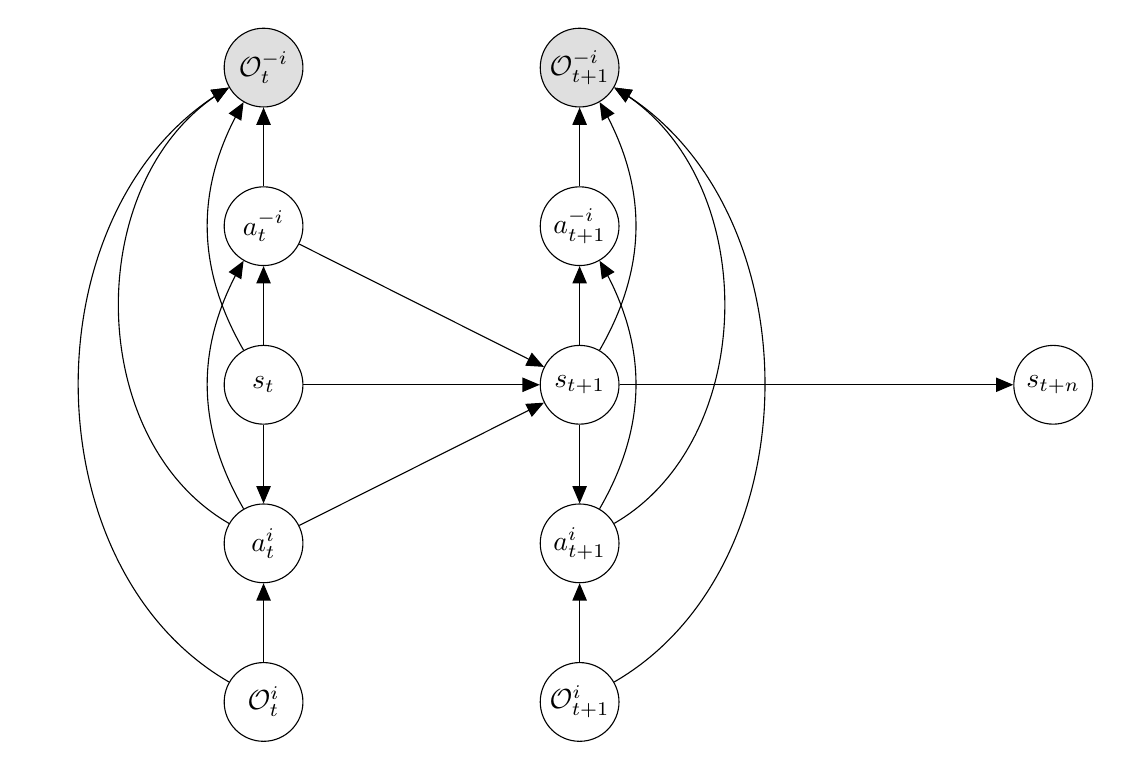
\begin{tikzpicture}[latent/.append style={minimum size=1.0cm}]
        \node[obs] (o1t) {$\mathcal{O}^{-i}_t$};
        \node[latent, below=of o1t] (a1t) {$a^{-i}_t$};
        \node[latent, below=of a1t] (st) {$s_t$};
        \node[latent, below=of st] (at) {$a^{i}_t$};
        \node[latent, below=of at] (ot) {$\mathcal{O}^{i}_t$};
        
        \edge {a1t} {o1t}
        \edge {st} {at, a1t}
        \edge {ot} {at}
        \path[->]  (ot)  edge   [bend left=60] node {} (o1t);
        \path[->]  (at)  edge   [bend left=30] node {} (a1t);
        \path[->]  (at)  edge   [bend left=60] node {} (o1t);
        \path[->]  (st)  edge   [bend left=30] node {} (o1t);
        
        \node[obs, right=3cm of o1t] (o1t1) {$\mathcal{O}^{-i}_{t+1}$};
        \node[latent, below=of o1t1] (a1t1) {$a^{-i}_{t+1}$};
        \node[latent, below=of a1t1] (st1) {$s_{t+1}$};
        \node[latent, below=of st1] (at1) {$a^{i}_{t+1}$};
        \node[latent, below=of at1] (ot1) {$\mathcal{O}^{i}_{t+1}$};
        
        \edge {a1t1} {o1t1}
        \edge {st1} {at1, a1t1}
        \edge {ot1} {at1}
        \path[->]  (ot1)  edge   [bend right=60] node {} (o1t1);
        \path[->]  (at1)  edge   [bend right=30] node {} (a1t1);
        \path[->]  (at1)  edge   [bend right=60] node {} (o1t1);
        \path[->]  (st1)  edge   [bend right=30] node {} (o1t1);
        
        \path[->]  (st)  edge   [] node {} (st1);
        \path[->]  (at)  edge   [] node {} (st1);
        \path[->]  (a1t)  edge   [] node {} (st1);
        
        \node[latent, right=5cm of st1] (stn) {$s_{t+n}$};
        \path[->]  (st1)  edge [] node {} (stn);
    \end{tikzpicture}
    \end{minipage}%
    \begin{minipage}[t]{0.5\linewidth}
    \caption{Graphical model that we want to approximate. For Balancing Q-learning, this is resemblance of PR2 graphical model. }
    \label{fig:chap3-balancing-Q-opponent}
    \end{minipage}
\end{figure}
This gives the following joint probability. The difference between PR2 and Balancing Q-learning is that we assume to have the knowledge of optimal action:
\begin{equation}
\begin{aligned}
    P(s_{1:T}, &a^i_{1:T}, a^{-i}_{1:T}, \optim^i_{1:T} = 1, \optim^{-i}_{1:T} = 1) \\
    &= P(s_0) \prod^T_{t=0} \pi_\theta(a^i_t | s_t, \optim^{i}_{t} = 1) P_{\prior}(a^{-i}_t | s_t, a^i_t) P(s_{t+1} | s_t, a^i_t, a^{-i}_t) P(\optim^{-i}_t = 1 | s_t, a^i_t, a^{-i}_t) P(\mathcal{O}^{-i}_t = 1)
\end{aligned}
\end{equation}
The variational joint probability is depicted as the following, the graphical model is very similar to figure \ref{fig:chap3-variational-ROMMEO} with difference condition on actions: 
\begin{equation}
    q(s_{1:T}, a_{1:T}^i, a^{-i}_{1:T}) = P(s_0) \prod^T_{t=0} \pi_\theta(a^i_t | s_t, \optim^{i}_{t} = 1) \rho_{\phi}(a^{-i}_t | s_t, a^i_t) P(s_{t+1} | s_t, a^i_t, a^{-i}_t)P(\optim^{-i}_t = 1)
\end{equation}
Given this, the optimality random variable is $P(\optim_t^{-i} = 1 | s_t, a^i_t, a^{-i}_t, \optim^{i}_t = 1)$ is defined as follows:
\begin{equation}
P(\optim_t^{-i} = 1 | s_t, a^i_t, a^{-i}_t, \optim^{i}_t = 1) \propto \exp \bracka{ \beta^{-i} r(s_t, a^i_t, a^{-i}_t)  }
\end{equation}
Now, we can see that the ELBO is simply:
\begin{equation}
    \mathbb{E}\brackb{\sum^T_{t=0} \beta^{-i} r(s_t, a^i_t, a^{-i}_t) - \log \frac{\rho_{\phi}(a^{-i}_t | s_t, a^i_t)}{ P_{\prior}(a^{-i}_t | s_t, a^i_t)}}
    % - \log \frac{\pi_{\theta}(a^{i}_t | s_t, \optim^{i}_{t} = 1)}{ P_{\prior}(a^{-i}_t | s_t, \optim^{i}_{t} = 1)}
\end{equation}
We can solve only for the opponent model, since we assume we have knowledge of agent's optimal policy. With the same working as ROMMEO and Balancing Q-learning, we arrived at the following policy definition:
\begin{equation}
\begin{aligned}
\label{eqn:chap3-prob-opponent}
    &\rho_{\phi}(a^{-i}_t | s_t, a^i_t) = \frac{\exp(Q(s_t, a^i_t, a^{-i}_t))P_\prior(a^{-i}_t | s_t, a^i_t)}{\exp(Q(s_t, a^{i}_t))} \\
    \text{ where }&Q(s_t, a^{i}_t) = \log \int \exp(Q(s_t, a^i_t, a^{-i}_t))P_\prior(a^{-i}_t | s_t, a^i_t) \dby a^{-i}_t \\
    % &Q(s_t, a^i_t, a^{-i}_t) = \beta^{-i} R(s_t, a^i_t, a^{-i}_t) + \gamma \mathbb{E}_{s_{t+1}, a^{i}_{t+1}\sim\pi_\theta}\brackb{Q(s_{t+1}, a^{i}_{t+1})}
\end{aligned}
\end{equation}
Now, please note that the definition of $Q(s_t, a^i_t, a^{-i}_t)$ isn't entirely correct because we are missing the regularization of the policy. We will left the action value as it be for now, once we have derived the agent's policy, let's re-calculate the action value function for more accurate value. Now, for policy, we have the following graphical model representation represented in figure \ref{fig:chap3-balancing-Q-agent}.
\begin{figure}[ht]
    \begin{minipage}[t]{0.5\linewidth}
    \centering
    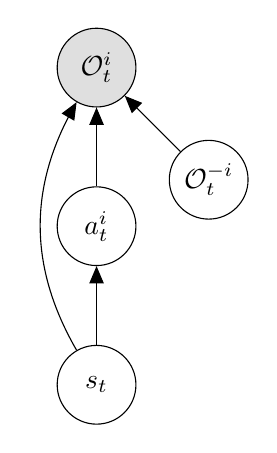
\begin{tikzpicture}[latent/.append style={minimum size=1.0cm}]
        \node[obs] (ot) {$\mathcal{O}^{i}_t$};
        \node[latent, below=of ot] (at) {$a^{i}_t$};
        \node[latent, below=of at] (st) {$s_t$};
        \node[latent, below right=of ot] (o1t) {$\mathcal{O}^{-i}_t$};
        % \node[latent, below=of st] (a1t) {$a^{-i}_t$};

        \edge {st} {at}
        \edge {at, o1t} {ot}
        % \path[->]  (a1t)  edge   [bend left=45] node {} (ot);
        % \path[->]  (a1t)  edge   [bend left=30] node {} (at);
        \path[->]  (st)  edge   [bend left=30] node {} (ot);
    \end{tikzpicture}
    \end{minipage}%
    \begin{minipage}[t]{0.5\linewidth}
    \caption{Graphical model that we want to approximate. This follows the VIREL \cite{fellows2019virel} type of graphical model rather than traditional probabilistic as inference framework.}
    \label{fig:chap3-balancing-Q-agent}
    \end{minipage}
\end{figure}
Given this, we define the optimality of an agent to be:
\begin{equation}
    P(\optim^{i}_t = 1 | s_t, a^{-i}_t, \optim^{-i}_t = 1) = \exp \bracka{ \frac{\beta^{i}}{\beta^{-i}} Q(s_t, a^{i}_t))  }
\end{equation}
Note that now, we assume the optimality of the opponent model via the use of soft-max of action value function this works when we are aware that the opponent will \correctquote{maximize} its action value function, and the fraction represents a conversion to agent's reward term. The variational probability is simply 
\begin{equation}
    q(s_t, a^{i}_t) = P(s_t) \pi_\theta(a^{i}_t | s_t)
\end{equation}
Therefore, the optimal opponent model is equal to 
\begin{equation}
\begin{aligned}
\label{eqn:chap3-prob-agent}
    &\pi_\theta(a^{i}_t | s_t) = \frac{\exp \bracka{ \cfrac{\beta^{i}}{\beta^{-i}} Q(s_t, a^{i}_t)} P_\prior(a^{i}_t | s_t)}{\exp\bracka{V^{i}(s_t)}} \\
    \text{ where }& V^{i}(s_t) = \log \int \exp \bracka{ \cfrac{\beta^{i}}{\beta^{-i}} Q(s_t, a^{i}_t)} P_\prior(a^{i}_t | s_t) \dby a^{-i}_t
\end{aligned}
\end{equation}
Now, let's consider the relationship between the $V^{i}(s_t)$, $Q(s_t, a_t^{i})$ and $Q(s_t, a^i_t, a^{-i}_t)$:
\begin{equation}
\label{eqn:chap3-prob-balance-val}
    V^{i}(s_t) = \mathbb{E}_{\pi, \rho}\brackb{\frac{\beta^{i}}{\beta^{-i}} Q(s_t, a^i_t, a^{-i}_t) - \frac{\beta^{i}}{\beta^{-i}}\log\frac{\rho_\phi(a^{-i}_t | s_t, a^i_t)}{P_\prior( a^{-i}_t| s_t, a^i_t)} - \log \frac{\pi_\theta(a^{i}_t | s_t)}{P_\prior(a^{i}_t | s_t)}}
\end{equation}
Given this, we can consider the corrected Q value as defined in following Bellman equation:
\begin{equation}
    Q(s_t, a^i_t, a^{-i}_t) = \beta^{-i} R(s_t, a^i_t, a^{-i}_t) + \gamma \mathbb{E}_{s_{t+1}}\brackb{\frac{\beta^{-i}}{\beta^i}V^{i}(s_{t+1})}    
\end{equation}
which we can used for the the calculation of opponent model. Now, we can see that by the use of the ratio between $\beta^{-i}$ and $\beta^{i}$, we can switch between the agent's action value function and opponent's action value function. Furthermore, from the use of extreamal operator in Bellman equation \cite{grau2018balancing} of Balancing Q-learning denotes similar notion to friend-or-foe learning \cite{littman2001friend}, which we can say that the Balancing Q-learning is the \correctquote{soft} version of friend-or-foe learning. The distinction between friend or foe is needed for the optimization of the agent.

\subsection{Implementation}
Now, we shall consider the implementation of the probabilistic Balancing Q-learning. Note that the current version of Balancing Q-learning based on discrete action, which we can find exact expected value. However, Balancing Q-learning can be implement in soft Actor-Critic like algorithm. The extension is trivial, while we are going to present similar algorithm, which is derived from the section before. This would require a total of 4 neural networks: $\pi_\theta(a^i_t | s_t, a^{-i}_t)$, $\rho_\phi(a^{-i}_t | s_t)$, $Q_\chi(s_t, a^i_t, a^{-i}_t)$ and $V_\psi(s_t)$. Let's consider the value function first. We will follows the definition of the value function that we have defined in equation \ref{eqn:chap3-prob-balance-val}, leading the following loss function:
\begin{equation}
    \mathcal{L}_V(\phi) = \mathbb{E}_{s_t} \brackb{\frac{1}{2}\bracka{V_{t}(s_t) - \mathbb{E}_{\pi_\theta, \rho_\phi}\brackb{\frac{\beta^{i}}{\beta^{-i}} Q_\chi(s_t, a^i_t, a^{-i}_t) - \frac{\beta^{i}}{\beta^{-i}}\log\frac{\rho_\phi(a^{-i}_t | s_t, a^i_t)}{P_\prior( a^{-i}_t| s_t, a^i_t)} - \log \frac{\pi_\theta(a^{i}_t | s_t)}{P_\prior(a^{i}_t | s_t)}} }^2}
\end{equation}
Now, we can use the Bellman equation of the action value function as the target for training:
\begin{equation}
    \mathcal{L}_Q(\chi) = \mathbb{E}_{s_t, a^{i}_t, a^{-i}_t, r_t, s_{t+1} \sim \mathcal{D}}\brackb{\frac{1}{2}\bracka{Q_\chi(s_t, a^{i}_t, a^{-i}_t) - \beta^{-i} r_t - \frac{\gamma\beta^{-i}}{\beta^i}V_\psi(s_{t+1})     }^2}
\end{equation}
Given the action value function, we can try to train the opponent model, which is in the form of $\rho_\phi(a^{-i}_t | s_t, a^i_t) = f^{-i}_\phi(\xi ; s_t, a^i_t)$ where the noise $\xi \sim \mathcal{N}(0, I)$. Given the function, we would like to minimizing the KL-divergence between the network's output and the closed form solution in equation \ref{eqn:chap3-prob-opponent} i.e minimizing the following objective 
\begin{equation}
    \mathcal{L}_\rho(\phi) = \kl\bracka{\rho_{\phi}(a^{-i}_t | s_t, a^i_t) \Bigg\| \frac{\exp(Q(s_t, a^i_t, a^{-i}_t))P_\prior(a^{-i}_t | s_t, a^i_t)}{\exp(Q(s_t, a^{i}_t))}}
\end{equation}
Now before we consider agent's objective, we will have to estimate the value $Q(s_t, a^{i}_t)$, which we are going to use Monte-Carlo estimate with importance sampling 
\begin{equation}
    Q^i(s_t, a^{i}_t) = \frac{\beta^{i}}{\beta^{-i}}\log \mathbb{E}_{a^{-i}_t \sim q}\brackb{\frac{\exp\bracka{Q(s_t, a^{i}_t, a^{-i}_t)} P_\prior(a^{-i}_t | s_t)}{q(a^{-i}_t)}}
\end{equation}
Given our estimation, we can now optimize the agent's policy $f^{i}_\theta(\xi ; s_t)$ by KL-divergence minimization based on equation \ref{eqn:chap3-prob-agent} as follows:
\begin{equation}
    \mathcal{L}_\pi(\theta) = \kl\bracka{\pi_\theta(a^{i}_t | s_t) \left\| \frac{\exp \bracka{Q^i(s_t, a^{i}_t)} P_\prior(a^i_t | s_t)}{\exp\bracka{V_\psi(s_t)}} \right.}
\end{equation}
This conclude the implementation of probabilistic Balancing Q-learning.

\Phu{TODO add ALGORITHM list and Gradient calculation}

\chapter{General Sum Extension}
\label{chapter:chap4}
\begin{miniabstract}
After we have a unified view on MAPI framework, which we have reinterpret Balancing Q-learning \cite{grau2018balancing} as a probabilistic inference. We are now going to consider extensions to agent's functionality. In this chapter, we are going to consider the case of temporal abstraction and communication in coopeartive multi-agent reinforcement learning problem. We will start by considering single agent option learning problem and solving it together with soft actor-critic like algorithm, as a minor contribution. After considering single agent problem, we are going to define a model in which the agent can plan and communicate and solving then.
\end{miniabstract}


\section{Single Agent Soft-Hierarchical Reinforcement Learning}
\label{sec:chap4-single-soft-HRL}
We will associate our model with option learning paradigm, and extends the result in \cite{igl2019multitask} by cooperating Soft-Actor Critic type solution as it is a standard method for solving probabilistic reinforcement learning. Furthermore, our approach is similar to \cite{daniel2016probabilistic}, in terms of using a similar probabilistic technique, however, in the paper, the authors concerning more on inferring policies from expert data, while didn't explicitly solve for each policy given the optimally condition (what we are trying to do now). Folloing \cite{igl2019multitask}, we have a master policy $\pi^H$ that suggesting the \correctquote{mode of execution} or an option to lower-level policy $\pi$ based on termination policy $\pi^T$, which tells what the next option should be. The joint distribution of actions i.e $P(s_{1:T}, a_{1:T}, \mathcal{O}_{1:T}, z_{1:T}, b_{1:T})$ is depicted in figure \ref{fig:chap4-single-agent-hierarchical}.
\begin{figure}[ht]
    \begin{minipage}[t]{0.5\linewidth}
    \centering
    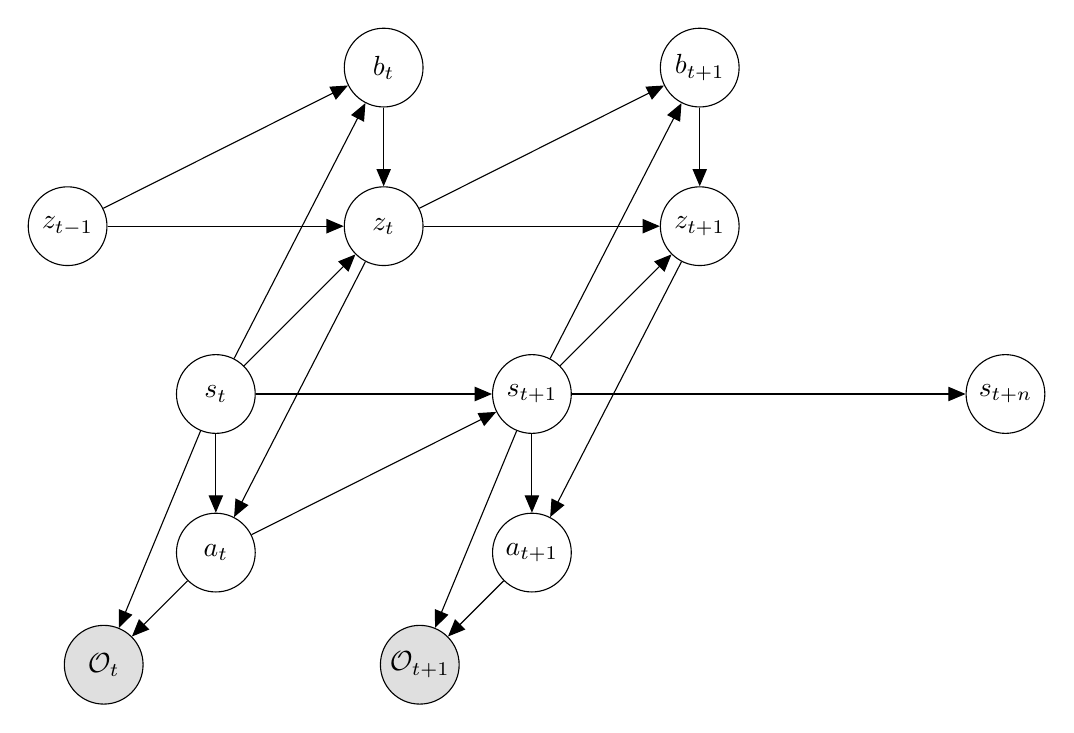
\begin{tikzpicture}[latent/.append style={minimum size=1.0cm}]
        \node[latent] (st) {$s_t$};
        \node[latent, below=of st] (at) {$a_t$};
        \node[latent, above right=2cm of st] (zt) {$z_t$};
        \node[latent, above=of zt] (bt) {$b_t$};
        \node[obs, below left=of at] (ot) {$\mathcal{O}_t$};
        
        \node[latent, left=3cm of zt] (zt-1) {$z_{t-1}$};
        
        % \edge{o1t} {a1t}
        \edge {st} {at, zt, bt}
        \edge {bt} {zt}
        \edge {zt}  {at}
        \edge {zt-1}  {bt, zt}
        \edge {at, st} {ot}
    
        \node[latent, right=3cmof st] (st1) {$s_{t+1}$};
        \node[latent, below=of st1] (at1) {$a_{t+1}$};
        \node[latent, above right=2cm of st1] (zt1) {$z_{t+1}$};
        \node[latent, above=of zt1] (bt1) {$b_{t+1}$};
        \node[obs, below left=of at1] (ot1) {$\mathcal{O}_{t+1}$};
        
        \edge {st, at} {st1}
        
        \edge {st1} {at1, zt1, bt1}
        \edge {bt1} {zt1}
        \edge {zt1}  {at1}
        \edge {zt}  {bt1, zt1}
        \edge {at1, st1} {ot1}
        
        \node[latent, right=5cm of st1] (stn) {$s_{t+n}$};
        \path[->]  (st1)  edge [] node {} (stn);
    \end{tikzpicture}
    \end{minipage}%
    \begin{minipage}[t]{0.5\linewidth}
    \caption{The the graphical model of hierarchical agent. We have the master policy which produces $z_t$ while having switch goal policy producing policy $b_t$}
    \label{fig:chap4-single-agent-hierarchical}
    \end{minipage}
\end{figure}
The joint distribution is then 
\begin{equation}
\begin{aligned}
    P(s_{1:T}, a_{1:T}, z_{1:T}, b_{1:T}) = P(s_0)P(z_0)\prod^T_{t=0} &P(s_{t+1} | s_t, a_t) P_\prior(a_t | s_t, z_t)\\
    &P_\prior^H(z_t | s_t, z_{t-1}, b_t) P_\prior^T(b_t | s_t, z_{t-1}) P(\mathcal{O}_t = 1 | s_t, a_t)
 \end{aligned}
\end{equation}
The variations joint distribution is defined as 
\begin{equation}
\begin{aligned}
    q(s_{1:T}, a_{1:T}, z_{1:T}, b_{1:T}) = P(s_0)P(z_0)\prod^T_{t=0} &P(s_{t+1} | s_t, a_t) \pi_{\theta}(a_t | s_t, z_t)\\
    &\pi^H_{\phi}(z_t | s_t, z_{t-1}, b_t) \pi^T_{\phi}(b_t | s_t, z_{t-1}) 
\end{aligned}
\end{equation}
Usually, the master policy and its prior are defined as. 
\begin{equation}
\begin{aligned}
    &\pi^H_{\phi}(z_t | s_t, z_{t-1}, b_t) = (1-b_t) \delta(z_t  - z_{t-1}) + b_t q^H_{\phi}(z_t | s_t) \\ 
    &P_\prior^H(z_t | s_t, z_{t-1}, b_t) = (1-b_t) \delta(z_t  - z_{t-1}) + b_t \frac{1}{m}
\end{aligned}
\end{equation}
As it takes the value of $b_t$ to suggest when to change the option $z_t$. Now, the ELBO is equal to 
\begin{equation}
    \mathbb{E}\brackb{\sum^T_{t=1} \beta r(s_t, a_t) - \log \frac{\pi_{\theta}(a_t | s_t, z_t)}{P_\prior(a_t | s_t, z_t)}  - \log \frac{\pi^H_{\phi}(z_t | s_t, z_{t-1}, b_t)}{P_\prior^H(z_t | s_t, z_{t-1}, b_t)} - \log \frac{\pi^T_{\phi}(b_t | s_t, z_{t-1}) }{P_\prior^T(b_t | s_t, z_{t-1})}}
\end{equation}
This objective is the same as the objective defined in \cite{igl2019multitask}. Given the ELBO, we will consider the closed-form solution of the low-level policy/master policy and termination policy. For the low-level policy, we have 
\begin{equation}
\begin{aligned}
\label{eqn:chap4-single-HRL-lower}
    &\pi_{\theta}(a_{t} | s_{t}, z_{t}) = \frac{P_\prior(a_{t} | s_{t}, z_{t})\exp\bracka{Q(s_{t}, a_{t}, z_{t})}}{\exp V(s_{t}, z_{t})} \\
    \text{ where }&V(s_{t}, z_{t}) = \log \int P_\prior(a_{t} | s_{t}, z_{t})\exp\bracka{Q(s_{t}, a_{t}, z_{t})} \dby a_{t}
\end{aligned}
\end{equation}
For the high-level policy, we have 
\begin{equation}
\begin{aligned}
\label{eqn:chap4-single-HRL-higher}
    &\pi^H(z_t | s_t) = \frac{\frac{1}{m}\exp\bracka{Q(s_t, z_t)}}{\exp\bracka{V(s_t)}}
    \\
    \text{ where } &Q(s_t, z_t) =  V(s_t, z_t)  \\
    &V^H(s_t) =  \frac{1}{m}\log \int \exp\bracka{Q(s_t, z_t)} \dby z_T
\end{aligned} 
\end{equation}
Finally, the termination policy is  
\begin{equation}
\begin{aligned}
\label{eqn:chap4-single-HRL-termination}
    &\pi^T(b_{t} | s_{t}, z_{t-1}) = \frac{P_\prior^T(b_{t} | s_{t}, z_{t-1})\exp{V(s_{t}, z_{t-1}, b_{t})}}{\exp V(s_{t}, z_{t-1})} \\
    \text{ where }& V(s_{t}, z_{t-1}, b_{t}) = b_{t} \brackb{V^H(s_{t})} + (1-b_{t})V(s_{t}, z_{t-1}) \\
    & V(s_{t}, z_{t-1}) = \log \int P_\prior^T(b_{t} | s_{t}, z_{t-1})\exp\bracka{b_{t} \brackb{V^H(s_{t})} + (1-b_{t})V(s_{t}, z_{t-1})} \dby b_{t}
\end{aligned}
\end{equation}
Finally, the Bellman equation for soft-hierarchical single-agent reinforcement learning is 
\begin{equation}
\label{eqn:chap4-single-HRL-bellman}
    Q(s_t, a_t, z_t) = \beta r(s_t, a_t) + \gamma\mathbb{E}_{s_{t+1}}\brackb{V(s_{t+1}, z_t)}
\end{equation}
The proof will be in appendix \ref{appx:chap4-soft-single-HRL}. We can see that this is analogous to the options framework \cite{sutton1999between, bacon2017option}. Now, we have aware the work on similar topic \cite{lobo2019soft}, which the authors have almost the same solution as us but miss specific points on value function calculation, notably 
\begin{equation}
\begin{aligned}
Q(s_t, a_t, z_t) = \beta r(s_t, a_t) + \mathbb{E}_{s_{t+1}}\Big[\mathbb{E}_{b_{t+1} \sim P(b_{t+1} | s_{t+1}, z_t), z_{t+1}' \sim P(z_{t+1} | s_{t+1})}\Big[&(1-b_{t+1})V(s_{t+1 }, z_t)  \\
&+ b_{t+1}V(s_{t+1 }, z_t')\Big]\Big]
\end{aligned}
\end{equation}
The authors fails to consider the case in which the master policy soft-max the value function $V(s_{t+1}, z_{t+1})$ and assuming this 
\begin{equation}
    \mathbb{E}_{z_{t+1}' \sim P(z_{t+1} | s_{t+1})}\brackb{V(s_{t+1}, z_{t+1})}
\end{equation}
Instead, which we can see that this misses the regularization of the policy $\pi^H_\phi$. By using the soft-max, we have implicitly included the regularization. 

\section{Multi-Agent Delayed Soft-Option Communication}
\label{sec:chap4-multi-soft-HRL-communication}
Now, we are going to consider the multi-agent case in which we have to consider the other agent's option at the last time step, which is a type of delayed communication, where the message is the option of the opponent. This algorithm would be a direct extension to the single-agent HRL problem. The graphical model can be too complex to draw we, therefore, going to show only the factorization of joint probabilities. Consider the following joint probability distribution of the problem:
\begin{equation}
\begin{aligned}
    P(&s_{1:T}, a^i_{1:T}, a^{-i}_{1:T}, z^i_{1:T}, z^{-i}_{1:T}, b^i_{1:T}, b^{-i}_{1:T}, \mathcal{O}^i_{1:T} = 1, \mathcal{O}^{-i}_{1:T} = 1) \\
    &= P(s_1)P(z^{-i}_0, z^i_0)\prod^T_{t=1} P(s_{t+1} | s_t, a_t^i, a_t^{-i})P_\prior(a^{-i}_t | s_t, z^i_t, a^i_t, z^{-i}_t) P^{H,-i}_\prior(z^{-i}_t | s_t, a^i_t, z^i_t, z^{-i}_{t-1}, b^i_t) \\
    &P^{T,-i}_\prior(b^{-i}_t | s_t,  z^{-i}_{t-1}, a^i_t, z^i_t) P_\prior(a^i_t | s_t, z^i_t, z^{-i}_{t-1}) P^{H,i}_\prior(z^i_t | s_t, z^{-i}_{t-1}, z^i_{t-1}, b^i_t) P^{T,i}_\prior(b^i_t | s_t, z^i_{t-1}, z^{-i}_{t-1})\\
    &P(\mathcal{O}^i_t = 1, \mathcal{O}^{-i}_t = 1 | s_t, a^i_t, a^{-i}_t)
\end{aligned}
\end{equation}
% \begin{itemize}
%     \item $P_\prior(a^i_t | s_t, z^i_t, a^{-i}_t, z^{-i}_t)$
%     \item $P^{H,i}_\prior(z^i_t | s_t, a^{-i}_t, z^{-i}_t)$
%     \item $P^{T,i}_\prior(b^i_t | s_t,  z^i_{t-1}, a^{-i}_t, z^{-i}_t)$
%     \item $P_\prior(a^{-i}_t | s_t, z^{-i}_t)$
%     \item $P^{H,-i}_\prior(z^{-i}_t | s_t, z^{-i}_{t-1}, b^{-i}_t)$
%     \item $P^{T,-i}_\prior(b^{-i}_t | s_t, z^{-i}_{t-1})$
% \end{itemize}
% WE HAVE
% \begin{itemize}
%     \item $P_\prior(a^{-i}_t | s_t, z^i_t, a^i_t, z^{-i}_t)$
%     \item $P^{H,-i}_\prior(z^{-i}_t | s_t, a^i_t, z^i_t, z^{-i}_{t-1}, b^i_t)$
%     \item $P^{T,-i}_\prior(b^{-i}_t | s_t,  z^{-i}_{t-1}, a^i_t, z^i_t)$
%     \item $P_\prior(a^i_t | s_t, z^i_t, z^{-i}_{t-1})$
%     \item $P^{H,i}_\prior(z^i_t | s_t, z^{-i}_{t-1}, z^i_{t-1}, b^i_t)$
%     \item $P^{T,i}_\prior(b^i_t | s_t, z^i_{t-1}, z^{-i}_{t-1})$
% \end{itemize}
Now, we shall consider the joint variational distribution. 
\begin{equation}
\begin{aligned}
    q(s_{1:T}, &a^i_{1:T}, a^{-i}_{1:T}, z^i_{1:T}, z^{-i}_{1:T}, b^i_{1:T}, b^{-i}_{1:T}, \mathcal{O}^{-i}_{1:T} = 1) \\
    &= P(s_1)P(z^{-i}_0, z^i_0)\prod^T_{t=1} q(s_{t+1} | s_t, a_t^i, a_t^{-i})\rho_\phi(a^{-i}_t | s_t, z^i_t, a^i_t, z^{-i}_t) q^{H,-i}(z^{-i}_t | s_t, a^i_t, z^i_t, z^{-i}_{t-1}, b^i_t) \\
    &q^{T,-i}(b^{-i}_t | s_t,  z^{-i}_{t-1}, a^i_t, z^i_t) \pi_\theta(a^i_t | s_t, z^i_t, z^{-i}_{t-1}) q^{H,i}(z^i_t | s_t, z^{-i}_{t-1}, z^i_{t-1}, b^i_t) q^{T,i}(b^i_t | s_t, z^i_{t-1}, z^{-i}_{t-1})
\end{aligned}
\end{equation}
Where we have the optimal random variable to be 
\begin{equation}
    P(\mathcal{O}^i_t = 1, \mathcal{O}^{-i}_{1:T} = 1 | s_t, a^i_t, a^{-i}_t) \propto \exp\bracka{\beta r(s_t, a_t^i, a^{-i}_t)}
\end{equation}
Before we move on, let's specifically define the master policy's conditional probability and its prior:
\begin{equation}
\begin{aligned}
    &q^{H, i}(z^i_t | s_t, z^{-i}_{t-1}, z^i_{t-1}, b^i_t) = (1-b_t^i) \delta(z_t^i  - z_{t-1}^i) + b_t^i q^{H, i}_{\phi}(z_t^i | s_t, z^{-i}_{T-1}) \\
    &P_\prior(z^i_t | s_t, z^{-i}_{t-1}, z^i_{t-1}, b^i_t) = (1-b_t^i) \delta(z_t^i  - z_{t-1}^i) + b_t^i \frac{1}{m} \\
    &q^{H, -i}(z^{-i}_t | s_t, a^i_t, z^i_t, z^{-i}_{t-1}, b^i_t) = (1-b_t^{-i}) \delta(z_t^{-i}  - z_{t-1}^{-i}) + b_t^{-i} q^{H, -i}_{\phi}(z_t^{-i} | s_t, a^i_t, z^i_t) \\
    &P_\prior(z^{-i}_t | s_t, a^i_t, z^i_t, z^{-i}_{t-1}, b^i_t) = (1-b_t^{-i}) \delta(z_t^{-i}  - z_{t-1}^{-i}) + b_t^{-i} \frac{1}{m} \\
\end{aligned}
\end{equation}
Given both of them, we can derive the ELBO by finding KL-divergence, which is equal to 
\begin{equation}
\begin{aligned}
    \mathbb{E}_q\Bigg[\sum^T_{t=0}\beta r(s_t, a_t^i, a^{-i}_t) &- \log\frac{\pi_\theta(a^i_t | s_t, z^i_t, z^{-i}_{t-1})}{P_\prior(a^i_t | s_t, z^i_t, z^{-i}_{t-1})} - \log\frac{\rho_\theta(a^{-i}_t | s_t, z^i_t, a^i_t, z^{-i}_t) }{P_\prior(a^{-i}_t | s_t, z^i_t, a^i_t, z^{-i}_t)} \\
    &- \log\frac{q^{H, i}(z^i_t | s_t, z^{-i}_{t-1}, z^i_{t-1}, b^i_t)}{P^{H, i}_\prior(z^i_t | s_t, z^{-i}_{t-1}, z^i_{t-1}, b^i_t)} - \log\frac{q^{H, -i}(z^{-i}_t | s_t, a^i_t, z^i_t, z^{-i}_{t-1}, b^i_t)}{P^{H, -i}_\prior(z^{-i}_t | s_t, a^i_t, z^i_t, z^{-i}_{t-1}, b^i_t)} \\
    &- \log\frac{q^{T,i}(b^i_t | s_t, z^i_{t-1}, z^{-i}_{t-1})}{P^{T,i}_\prior(b^i_t | s_t, z^i_{t-1}, z^{-i}_{t-1})} - \log\frac{q^{T,-i}(b^{-i}_t | s_t,  z^{-i}_{t-1}, a^i_t, z^i_t)}{P^{T,-i}_\prior(b^{-i}_t | s_t,  z^{-i}_{t-1}, a^i_t, z^i_t) } \Bigg]
\end{aligned}
\end{equation}
% \begin{itemize}
%     \item $P_\prior(a^{-i}_t | s_t, z^i_t, a^i_t, z^{-i}_t)$
%     \item $P^{H,-i}_\prior(z^{-i}_t | s_t, a^i_t, z^i_t, z^{-i}_{t-1}, b^i_t)$
%     \item $P^{T,-i}_\prior(b^{-i}_t | s_t,  z^{-i}_{t-1}, a^i_t, z^i_t)$
%     \item $P_\prior(a^i_t | s_t, z^i_t, z^{-i}_{t-1})$
%     \item $P^{H,i}_\prior(z^i_t | s_t, z^{-i}_{t-1}, z^i_{t-1}, b^i_t)$
%     \item $P^{T,i}_\prior(b^i_t | s_t, z^i_{t-1}, z^{-i}_{t-1})$
% \end{itemize}
We will show the full working for solving in appendix \ref{appx:chap4-soft-multi-HRL}. Now, the policies are: starting with opponent model's policy 
\begin{equation*}
\begin{aligned}
    &\rho(a^{-i}_t | s_t, z^i_t, a^{i}_t, z^{-i}_t) = \frac{\exp Q(s_t, z^i_t, a^{i}_t, z^{-i}_t, a^{-i}_t) P_\prior(a^{-i}_t | s_t, z^i_t, a^{i}_t, z^{-i}_t)}{\exp Q(s_t, z^i_t, a^{i}_t, z^{-i}_t)} \\
    \text{ where } &Q(s_t, z^i_t, a^{i}_t, z^{-i}_t) = \log \int \exp Q(s_t, z^i_t, a^{i}_t, z^{-i}_t, a^{-i}_t) P_\prior(a^{-i}_t | s_t, z^i_t, a^{i}_t, z^{-i}_t) \dby a^{-i}_t
\end{aligned}
\end{equation*}
Now, the opponent's master policy is 
\begin{equation}
\begin{aligned}
    &q^{H, -i}(z_t^{-i} | s_t, a^i_t, z^i_t) = \frac{\exp Q(s_t, z^i_t, a^{i}_t, z^{-i}_t) P_\prior(z_t^{-i} | s_t, a^i_t, z^i_t)}{\exp Q(s_t, z^i_t, a^{i}_t)} \\
    \text{ where }& Q(s_t, z^i_t, a^{i}_t) = \log \int \exp Q(s_t, z^i_t, a^{i}_t, z^{-i}_t) P_\prior(z_t^{-i} | s_t, a^i_t, z^i_t) \dby z^{-i}_t
\end{aligned}
\end{equation}
And, the opponent's terminal policy is 
\begin{equation}
\begin{aligned}
    &q^{T,-i}(b^{-i}_t | s_t,  z^{-i}_{t-1}, a^i_t, z^i_t) = \frac{\exp Q(s_t,  z^{-i}_{t-1}, a^i_t, z^i_t, b^{-i}_t) P_\prior(b^{-i}_t | s_t,  z^{-i}_{t-1}, a^i_t, z^i_t)}{\exp Q(s_t,  z^{-i}_{t-1}, a^i_t, z^i_t)} \\
    \text{ where }&Q(s_t,  z^{-i}_{t-1}, a^i_t, z^i_t, b^{-i}_t) = b^{-i}_t\brackb{Q(s_t, z^i_t, a^{i}_t)} + (1-b^{-i}_t)\brackb{Q(s_t, z^i_t, a^{i}_t, z^{-i}_{t-1})} \\
    &Q(s_t,  z^{-i}_{t-1}, a^i_t, z^i_t) = \log \int \exp Q(s_t,  z^{-i}_{t-1}, a^i_t, z^i_t, b^{-i}_t) P_\prior(b^{-i}_t | s_t,  z^{-i}_{t-1}, a^i_t, z^i_t) \dby b^{-i}_t
\end{aligned}
\end{equation}
Now, we shifted to agent's policy, which is equal to 
\begin{equation}
\begin{aligned}
    &\pi(a^i_t | s_t, z^i_t, z^{-i}_{t-1}) = \frac{\exp Q(s_t,  z^{-i}_{t-1}, a^i_t, z^i_t) P_\prior(a^i_t | s_t, z^i_t, z^{-i}_{t-1})}{\exp Q(s_t,  z^{-i}_{t-1}, z^i_t)} \\
    \text{ where }&Q(s_t,  z^{-i}_{t-1}, z^i_t) = \log \int \exp Q(s_t,  z^{-i}_{t-1}, a^i_t, z^i_t) P_\prior(a^i_t | s_t, z^i_t, z^{-i}_{t-1}) \dby a^i_t
\end{aligned}
\end{equation}
The master policy for the agent follows the agent's value function
\begin{equation}
\begin{aligned}
    &q^{H, i}(z_t^i | s_t, z^{-i}_{t-1}) = \frac{\exp Q(s_t,  z^{-i}_{t-1}, z^i_t) P_\prior(z_t^i | s_t, z^{-i}_{t-1})}{\exp Q(s_t,  z^{-i}_{t-1})} \\
    \text{ where }&Q(s_t,  z^{-i}_{t-1}) = \log \int\exp Q(s_t,  z^{-i}_{t-1}, z^i_t) P_\prior(z_t^i | s_t, z^{-i}_{t-1}) \dby z_t^i
\end{aligned}
\end{equation}
Finally, ends with the agent termination policy with left us the the message.
\begin{equation}
\begin{aligned}
    &q^{T,i}(b^i_t | s_t, z^i_{t-1}, z^{-i}_{t-1}) = \frac{\exp Q(s_t, z^i_{t-1}, z^{-i}_{t-1}, b^i_t) P_\prior(b^i_t | s_t, z^i_{t-1}, z^{-i}_{t-1})}{\exp Q(s_t, z^i_{t-1}, z^{-i}_{t-1}) } \\
    \text{ where }&Q(s_t, z^i_{t-1}, z^{-i}_{t-1}, b^i_t)  = b^i_t\brackb{Q(s_t,  z^{-i}_{t-1})} + (1-b^i_t)\brackb{Q(s_t,  z^{-i}_{t-1}, z^i_{t-1})} \\
    &Q(s_t, z^i_{t-1}, z^{-i}_{t-1}) = \log \int \exp Q(s_t, z^i_{t-1}, z^{-i}_{t-1}, b^i_t) P_\prior(b^i_t | s_t, z^i_{t-1}, z^{-i}_{t-1}) \dby b^i_t
\end{aligned}
\end{equation}
Now, finally the bellman equation is 
\begin{equation}
    Q(s_t, a_t^i, a^{-i}_t, z^i_{t}, z^{-i}_{t} ) = \beta r(s_t, a_t^i, a^{-i}_t) + \gamma\mathbb{E}_{s_{t+1}}\brackb{Q(s_{t+1}, z^i_{t}, z^{-i}_{t})}
\end{equation}
Note that this is similar to the one proposed to \cite{han2019multi}. The agent's policy can be executed by message $z_{t-1}^{-i}$ sent from the opponent. This process is also exciting since by having the message from an opponent, the agent can anticipate what the opponent can do next, which is shown in the calculation of the action-value function, and the agent can also understand how the message would affect the opponent's action.

\section{Implementation}
Now, we have consider the implementation of the algorithms starting with the implementation of single agent learning, and this can be easily extends to multi-agent problem. The purpose of this section is to show that Soft Actor-Critic like algorithm can be applied directly to the implementation of the algorithms. Finally, we will not go through the tricks that would stabilize the training since we are focusing on the control as probabilistic framework extensions and proves that the implementation is possible by constructing one.
 
\subsection{Single agent problem}
Starting with the value function $V(s_t, z_t)$, which we can train using the following :
\begin{equation}
    \mathcal{L}_{V_1} = \mathbb{E}_{s_t, z_t \sim \mathcal{D}} \brackb{\frac{1}{2}\bracka{V(s_t, z_t) - \mathbb{E}_{a_t \sim \pi_\theta(a_t | s_t, z_t)}\brackb{Q(s_t, a_t, z_t) - \log \frac{\pi_\theta(a_t | s_t, z_t)}{P_\prior(a_t | s_t, z_t)}}}^2}
\end{equation}
Similarly, the value function $V(s_t)$ can be trained to 
\begin{equation}
    \mathcal{L}_{V_2} = \mathbb{E}_{s_t \sim \mathcal{D}}\brackb{\frac{1}{2}\bracka{V(s_t) - \mathbb{E}_{z_t \sim \pi^H(z_t | s_t)}\brackb{V(s_t, z_t) - \log\bracka{m\cdot \pi^H(z_t | s_t)}}}^2}
\end{equation}
Finally, we can train the value function for the termination policy $V(s_t, z_{t-1})$ as:
\begin{equation}
    \mathcal{L}_{V_3} = \mathbb{E}_{s_t, z_{t-1} \sim \mathcal{D}}\brackb{\frac{1}{2}\bracka{V(s_t, z_{t-1}) - \mathbb{E}_{b_t \sim \pi^T(b_t | s_t, z_{t-1})}\brackb{ V(s_t, z_{t-1}, b_t) - \log \frac{\pi^T(b_t | s_t, z_{t-1})}{P_\prior(b_t | s_t, z_{t-1})}}  }}
\end{equation}
Now, lower level policy is in the form of $a_t = f^L(\xi ; s_t, z_t)$ where $\xi \sim \mathcal{N}(0, I)$, we can train it to minimize the KL-divergence between this to the optimal policy that we have shown in equation \ref{eqn:chap4-single-HRL-lower} as
\begin{equation}
    \mathcal{L}_{\pi^L} = \kl\bracka{\pi^L(a_t | s_t, z_t) \Bigg\| \frac{P_\prior(a_{t} | s_{t}, z_{t})\exp\bracka{Q(s_{t}, a_{t}, z_{t})}}{\exp V(s_{t}, z_{t})}}
\end{equation}
Similarly, the higher-level policy will be in the form of $z_t = f^H(\xi ; s_t)$ where $\xi \sim \mathcal{N}(0, I)$ with the following KL-divergence objective from the optimal policy equation \ref{eqn:chap4-single-HRL-higher}:
\begin{equation}
    \mathcal{L}_{\pi^H} = \kl\bracka{\pi^H(z_t | s_t) \Bigg\| \frac{\exp\bracka{Q(s_t, z_t)}}{m\exp\bracka{V(s_t)}}}
\end{equation}
And the termination policy is in the form of $b_t = \sigma(f^T(\xi ; s_t, z_{t-1}))$, where $\sigma$ denotes the Sigmoid function, which transforms the output to be between $0$ and $1$. We still use the KL-divergence objective derived from equation \ref{eqn:chap4-single-HRL-termination}:
\begin{equation}
    \mathcal{L}_{\pi^T} = \kl\bracka{\pi^T(b_t | s_t, z_{t-1}) \Bigg\| \frac{P_\prior^T(b_{t} | s_{t}, z_{t-1})\exp{V(s_{t}, z_{t-1}, b_{t})}}{\exp V(s_{t}, z_{t-1})} }
\end{equation}
Finally, we can train the action value function $Q(s_t, a_t, z_t)$, which is calculated via the Bellman equation \ref{eqn:chap4-single-HRL-bellman} as:
\begin{equation}
    \mathcal{L}_Q = \mseloss{(s_t, a_t, z_t, r_t, s_{t+1}) \sim \mathcal{D}}{Q(s_t, a_t, z_t)}{\beta r(s_t, a_t) + \gamma V(s_{t+1}, z_t)}
\end{equation}

\subsection{Multi agent problem}
Since there are lots of objective to follows, we will list them down here. The technique used is the same as one proposed in single agent case. We shall start with the definition of the value function 
\begin{itemize}
    \item Opponent's lower level policy value function $Q(s_t, z^i_t, z^{-i}_t, a^i_t)$:
    \begin{equation}
        \mathcal{L}_{Q_1} = \mseloss{(s_t, z^i_t, z^{-i}_t, a^i_t, a^i_t) \sim \mathcal{D}}{Q(s_t, z^i_t, z^{-i}_t)}{\mathbb{E}_{a^{-i}_t}\brackb{Q(s_t, z^i_t, a^i_t, z^{-i}_t, a^{-i}_t) - \log\frac{ \rho(a^{-i}_t | s_t, z^i_t, z^{-i}_t, a^i_t)}{P_\prior(a^{-i}_t | s_t, z^i_t, z^{-i}_t, a^i_t)}}}
    \end{equation}
    where the opponent model action is sampled from $a^{-i}_t \sim \rho(a^{-i}_t | s_t, z^i_t, z^{-i}_t, a^i_t)$.
    \item Opponent's master policy value function $Q(s_t, z^i_t)$:
    \begin{equation}
        \mathcal{L}_{Q_2} = \mseloss{(s_t, z^i_t, z^{-i}_t) \sim \mathcal{D}}{Q(s_t, z^i_t)}{\mathbb{E}_{z^{-i}_t}\brackb{Q(s_t, z^i_t, z^{-i}_t) - \log\frac{q^{H, -i}(z^{-i}_t | s_t, z^i_t)}{P_\prior(z^{-i}_t | s_t, z^i_t)}}}
    \end{equation}
    where the option is sampled from $z^{-i}_t \sim q^{H, -i}(z^{-i}_t | s_t, z^i_t)$.
    \item Opponent's termination policy value function $Q(s_t, z^{-i}_{t-1}, a^i_t, z^i_t)$:
    \begin{equation}
        \mathcal{L}_{Q_3} = \mseloss{(s_t, z^{-i}_{t-1}, a^i_t, z^i_t) \sim \mathcal{D}}{Q(s_t, z^{-i}_{t-1}, a^i_t, z^i_t)}{\mathbb{E}_{b^{-i}_t}\brackb{Q(s_t,  z^{-i}_{t-1}, a^i_t, z^i_t, b^{-i}_t) - \log\frac{q^{T,-i}(b^{-i}_t | s_t,  z^{-i}_{t-1}, a^i_t, z^i_t) }{P_\prior(b^{-i}_t | s_t,  z^{-i}_{t-1}, a^i_t, z^i_t) }}}
    \end{equation}
    where the terminating signal is sampled from $b^{-i}_t \sim q^{T,-i}(b^{-i}_t | s_t,  z^{-i}_{t-1}, a^i_t, z^i_t)$.
    \item Agent's lower level policy value function $Q(s_t,  z^{-i}_{t-1}, z^i_t)$:
    \begin{equation}
        \mathcal{L}_{Q_4} = \mseloss{(s_t,  z^{-i}_{t-1}, z^i_t) \sim \mathcal{D}}{Q(s_t,  z^{-i}_{t-1}, z^i_t)}{\mathbb{E}_{a^i_t}\brackb{Q(s_t,  z^{-i}_{t-1}, a^i_t, z^i_t)  - \frac{\pi(a^i_t | s_t, z^i_t, z^{-i}_{t-1})}{P_\prior(a^i_t | s_t, z^i_t, z^{-i}_{t-1})}}}
    \end{equation}
    where the lower level action is sampled from $a^i_t \sim \pi(a^i_t | s_t, z^i_t, z^{-i}_{t-1})$
    \item Agent's master policy value function $Q(s_t,  z^{-i}_{t-1})$:
    \begin{equation}
        \mathcal{L}_{Q_5} = \mseloss{(s_t,  z^{-i}_{t-1})\sim \mathcal{D}}{Q(s_t,  z^{-i}_{t-1})}{\mathbb{E}_{z^i_t}\brackb{Q(s_t,  z^{-i}_{t-1}, z^i_t) - \log\frac{q^{H, i}(z_t^i | s_t, z^{-i}_{t-1})}{P_\prior(z_t^i | s_t, z^{-i}_{t-1})}}}
    \end{equation}
    where the agent's option is sampled from $z_t^i \sim q^{H, i}(z_t^i | s_t, z^{-i}_{t-1})$
    \item Finally, agent's termination policy value function $Q(s_t, z^i_{t-1}, z^{-i}_{t-1})$:
    \begin{equation}
        \mathcal{L}_{Q_6} = \mseloss{}{Q(s_t, z^i_{t-1}, z^{-i}_{t-1})}{\mathbb{E}_{b^i_t}\bracka{Q(s_t, z^i_{t-1}, z^{-i}_{t-1}, b^i_t) - \log \frac{q^{T, i}(b^i_t | s_t, z^i_{t-1}, z^{-i}_{t-1})}{P_\prior(b^i_t | s_t, z^i_{t-1}, z^{-i}_{t-1})}}}
    \end{equation}
    where the agent's terminating condition is sampled from $b^i_t \sim q^{T, i}(b^i_t | s_t, z^i_{t-1}, z^{-i}_{t-1})$
\end{itemize}
Now, we have listed all the agent's and its opponent model's value function, we can now consider the policies objective. 
\begin{itemize}
    \item Opponent Model's lower level policy $a^{-i}_t = f(\xi ; s_t, z^i_t, a^{i}_t, z^{-i}_t)$
    \begin{equation}
        \mathcal{L}_{\rho} = \klloss{\rho_\theta(a^{-i}_t | s_t, z^i_t, a^{i}_t, z^{-i}_t)}{ \frac{\exp Q(s_t, z^i_t, a^{i}_t, z^{-i}_t, a^{-i}_t) P_\prior(a^{-i}_t | s_t, z^i_t, a^{i}_t, z^{-i}_t)}{\exp Q(s_t, z^i_t, a^{i}_t, z^{-i}_t)}}
    \end{equation}
    \item Opponent Model's master policy $z^{-i}_t = f^{H, -i}(\xi;  s_t, a^i_t, z^i_t)$
    \begin{equation}
        \mathcal{L}_{q^{H, -i}} = \klloss{q^{H, -i}(z_t^{-i} | s_t, a^i_t, z^i_t)}{\frac{\exp Q(s_t, z^i_t, a^{i}_t, z^{-i}_t) P_\prior(z_t^{-i} | s_t, a^i_t, z^i_t)}{\exp Q(s_t, z^i_t, a^{i}_t)}}
    \end{equation}
    \item Opponent Model's termination policy $b^{-i}_t= f^{T, -i}(\xi; s_t,  z^{-i}_{t-1}, a^i_t, z^i_t)$
    \begin{equation}
        \mathcal{L}_{q^{T,-i}} = \klloss{q^{T,-i}(b^{-i}_t | s_t,  z^{-i}_{t-1}, a^i_t, z^i_t)}{\frac{\exp Q(s_t,  z^{-i}_{t-1}, a^i_t, z^i_t, b^{-i}_t) P_\prior(b^{-i}_t | s_t,  z^{-i}_{t-1}, a^i_t, z^i_t)}{\exp Q(s_t,  z^{-i}_{t-1}, a^i_t, z^i_t)}}
    \end{equation}
    \item Agent lower level policy $a^i_t= f(\xi; s_t, z^i_t, z^{-i}_{t-1})$
    \begin{equation}
        \mathcal{L}_{\pi} = \klloss{ \pi_\theta(a^i_t | s_t, z^i_t, z^{-i}_{t-1})}{\frac{\exp Q(s_t,  z^{-i}_{t-1}, a^i_t, z^i_t) P_\prior(a^i_t | s_t, z^i_t, z^{-i}_{t-1})}{\exp Q(s_t,  z^{-i}_{t-1}, z^i_t)}}
    \end{equation}
    \item Agent master policy $z^i_t= f^{H, i}(\xi; s_t, z^{-i}_{t-1})$
    \begin{equation}
        \mathcal{L}_{q^{H, i}} = \klloss{q^{H, i}(z_t^i | s_t, z^{-i}_{t-1})}{\frac{\exp Q(s_t,  z^{-i}_{t-1}, z^i_t) P_\prior(z_t^i | s_t, z^{-i}_{t-1})}{\exp Q(s_t,  z^{-i}_{t-1})}}
    \end{equation}
    \item agent termination policy $b^i_t= f^{T, i}(\xi;s_t, z^i_{t-1}, z^{-i}_{t-1})$
    \begin{equation}
        \mathcal{L}_{q^{T,i}} = \klloss{q^{T,i}(b^i_t | s_t, z^i_{t-1}, z^{-i}_{t-1})}{\frac{\exp Q(s_t, z^i_{t-1}, z^{-i}_{t-1}, b^i_t) P_\prior(b^i_t | s_t, z^i_{t-1}, z^{-i}_{t-1})}{\exp Q(s_t, z^i_{t-1}, z^{-i}_{t-1}) }}
    \end{equation}
\end{itemize}
Note that all the noises is sampled from normal distribution $\xi \sim \mathcal{N}(0, I)$. Finally, the action value function $Q(s_t, z^i_t, a^i_t, z^{-i}_t, a^{-i}_t)$:
\begin{equation}
    \mathcal{L}_{Q} = \mseloss{(s_t, z^i_t, a^i_t, z^{-i}_t, a^{-i}_t, r_t, s_{t+1}) \sim \mathcal{D}}{Q(s_t, z^i_t, a^i_t, z^{-i}_t, a^{-i}_t)}{\beta r(s_t, a_t^i, a^{-i}_t) + \gamma \mathbb{E}{Q(s_{t+1}, z^i_{t}, z^{-i}_{t})}}
\end{equation}




\chapter{EM-Algorithm For Multi-Agent Reinforcement Learning}
\label{chapter:chap5}
\begin{miniabstract}
Another crucial extension to the multi-agent policy would be the ability to infer the hidden state via its local information. We will consider the cooperative case in which the agent's action is available as part of \correctquote{public observation}. The main observation from \cite{nayyar2013decentralized, foerster2018bayesian} is that we can turn partially observable multi-agent problem into single-agent POMDP by considering the public agent that forms a belief of the state given histories of public observation. Given its belief over the state, the public agent constructs a placeholder policy that acts according to each agents' individual observation. By having the same placeholder policy for all agents, we ensure that all the agents are coordinated correctly. We will start by introducing the Public Belief MDP framework. Then we introduce Variational Sequential Monte Carlo (VSMC) \cite{le2017auto, maddison2017filtering, naesseth2017variational}, which is a basis to Deep Variational Reinforcement Learning (DVRL) \cite{igl2018deep} - an algorithm that captures the belief overstate. We will follow \cite{shvechikovjoint} on the control as a probabilistic framework interpretation of DVRL to construct our multi-agent algorithms.
\end{miniabstract}

\section{Public Belief MDP}
\label{sec:chap5-pub-belief-MDP}
As we aware, recursive learning in many steps can be complex and expensive even in cooperation problem. By using public agent formulation, we can reduce the problem into single agent POMDP task, which would be easier to manage. This technique is proposed in \cite{nayyar2013decentralized} and extended to scale over by approximation and neural network in \cite{foerster2018bayesian}. 

The public belief MDP is based on the fact that every agent can some how infer the underlying state given a public observation (can also be an action too). After forming such a belief, each agent can executes and action that condition on its private observation and the belief over the state. Given a decoupled process, we can have a centralized agent that only infer the underlying state and distribute the common belief to each lower level agent to execute its action. The process can be summarized as follows:
\begin{itemize}
    \item The higher-level agent observers a public observation and construct a message $m_t \sim \pi^{\pri}_t(\cdot | o^{\pub}_t, a^{\pub}_t)$ with state distribution $\mathcal{B}_t = P(s_t | o^{\pub}_{\le t})$ where $o^{\pub}_{\le t}$ is the history of public policy till time $t$
    \item The lower-level agent after receives the message from the higher-level agent will execute its action based on its private observation, the message given, and belief over state calculated using higher-level agent i.e $a^i_t \sim \pi^i(\cdot | m_t, \mathcal{B}_t, o^{\pri}_t)$. 
\end{itemize}
Please note that by having a centralized public belief agent makes the coordination problem much easier since the each agent can reason about the other's action based on its the belief of other agent's private observation conditioned on message $m_t$. And, both of the agent and its higher-level counter part will try to optimize the same reward. Note that we can train the public agent individually for each agent however we have to make sure that they are the same, which can be implemented by a public seed \cite{foerster2018bayesian}.

\section{Variational Sequential Monte Carlo and Deep Variational Reinforcement Learning}
\label{sec:chap5-VSMC-DVL}

\subsection{VSMC}
Let's start with Importance-Weight Auto Encoder \cite{burda2015importance}. Consider the Jensen equality derivation of ELBO, where we can show that 
\begin{equation}
    \log P(X) = \log \bracka{\int P(X, z) \dby z}  = \log \bracka{\int P(z|X) P(X) \dby z} = \log \bracka{\mathbb{E}_{P(z | X)}\brackb{P(X)}}
\end{equation}
Now, given the expected value, we can use our variational distribution $q_\phi(z)$ to be our importance sampling distribution i.e
\begin{equation}
\begin{aligned}
    \log \mathbb{E}_{q_\phi(z |x)}\brackb{\frac{P(z | X)}{q_\phi(z |x)} P(X)} &= \log \mathbb{E}_{q_\phi(z |x)}\brackb{\frac{P(X, z)}{q_\phi(z |x)}} \\
    &= \log \mathbb{E}_{z_1, \dots, z_K}\brackb{\frac{1}{K}\sum^K_{k=1} \frac{P(X, z)}{q_\phi(z |x)}} \ge \mathbb{E}\brackb{\log \frac{1}{K}\sum^K_{k=1} \frac{P(X, z)}{q_\phi(z |x)}}
\end{aligned}
\end{equation}
We will now generalize the result from IWAE by using the notion of Monte Carlo objective \cite{maddison2017filtering}, where we define the denote positive estimator of $P(x)$ as $\hat{P}_N(x)$. Then, the Monte Carlo objective (which is always a lower bound of $P(x)$) is defined as 
\begin{equation}
\label{eqn:chap5-elbo-general}
    \mathbb{E}[\log \hat{p}_N(x)]
\end{equation}
For a hidden Markov model, we can simply calculate the $P(x_{1:T})$ where $x_t$ is an observable variable using Sequential Monte Carlo (SMC) \cite{doucet2001introduction} we can train variational emission distribution and transition distribution using a lower bound in equation \ref{eqn:chap5-elbo-general} via back-propagation.  

\subsection{DVRL}
Typically, in reinforcement learning, we usually use a recurrent neural network (RNN) to encode the state to $h_t$ condition of the past action and observation. Given the RNN state $h_t$ we can then condition our policy on $h_t$. However, this only works because of memory and heuristic from RNN. DVRL aim to solve POMDP by 
\begin{itemize}
    \item Estimating the transition and observation model 
    \item Perform an inference model 
    \item Choosing an action based on inferred belief state.
\end{itemize}
The authors uses 3 elements triplet $(h^k_t, z^k_t, w^k_t)$ where $h^k_t$ is the latent of RNN, $z^k_t$ is the additional stochastic latent state and $w^k_t$ is the weight, as a particle. The belief is the updated, at time $t$, as follows 
\begin{equation}
\begin{aligned}
    &u^k_{t-1} \sim \text{Categorical}\bracka{\frac{w^k_{t-1}}{\sum^K_{k=1}w^k_{t-1}}} \\
    &z^k_{t} \sim q_{\phi}(z^k_t | h^{u^k_{t-1}}_{t-1}, a_{t-1}, o_t) \\
    &h^k_t = \psi^{\text{RNN}}_\theta (h^{u^k_{t-1}}_{t-1}, z^k_t, a_{t-1}, o_t) \\
    &w^k_T = \frac{P_\theta(z^k_t | h^{u^k_{t-1}}_{t-1}) P_\theta(o_t | h^{u^k_{t-1}}_{t-1}, z^k_t, a_{t-1})}{q_\phi(z^k_t | h^{u^k_{t-1}}_{t-1}, a_{t-1}, o_t)}
\end{aligned}
\end{equation}
The model of the world is trained via ELBO 
\begin{equation}
    \mathcal{L}^{ELBO}_{t}(\theta, \phi) = -\frac{1}{n_en_s} \sum^{n_e}_{\text{envs}} \sum^{n_s - 1}_{i=0} \log \bracka{\frac{1}{K}\sum^K_{k=1}w^k_{t+i}}
\end{equation}
The agent executes its action $\pi(a_t | \hat{h}_t)$ \footnote{and calculate its value, since it is Actor-Critic model} by using another RNN to aggregate all the history of particles, which returns $\hat{h}_t$ . The agent's reward and its model of the world are trained \textit{jointly}f\footnote{We disagree with \cite{huangsvqn} when the authors claim that \cite{igl2018deep} \correctquote{separate the planning algorithm and the inference of the hidden state.}, since \cite{igl2018deep} claims in the abstract that DVRL \correctquote{allowing the model to be trained jointly with the policy.}} using back-propagation through time (BPTT) via standard Actor-Critic framework. For more information on BPTT training for the agent, we refer to the paper for more details. \cite{shvechikovjoint} has proposed a graphical model representation of the problem, while showing that a similar algorithm could be derived from control as inference framework. The major difference is how the agent's action is calculated. As mentioned before \cite{igl2018deep} uses secondary RNN to aggregate the histories to inform the agent, however, \cite{shvechikovjoint} uses a weighted average on the action of the agent over its belief over state i.e
\begin{equation}
    \sum^K_{k=1} \frac{w^k_{t}}{\sum^K_{k=1}w^k_{t}} \pi(a_t | h_t^k)
\end{equation}
Another work on using control as inference framework is \cite{huangsvqn}. The authors also consider optimizing ELBO objective. However, we believe that \cite{shvechikovjoint} provides more general solution since once the number of particle is equal to one, ELBO derived in \cite{huangsvqn}\footnote{See equation 19 in appendix of \cite{huangsvqn}} is similar to \cite{shvechikovjoint}\footnote{See equation 4 in appendix of \cite{shvechikovjoint}}/ELBO from multiple. Furthermore, by having multiple possibilities of hidden state with its weight, we can consider a counter-factual in multi-agent scenario, thus being more useful than one state representation. Finally, the difference between \cite{huangsvqn} and \cite{shvechikovjoint} lies in the use of VAE like objective when considering state transition, as \cite{huangsvqn} minimizes VAE objective for state representation as an auxiliary loss, while \cite{shvechikovjoint} doesn't and focuses on maximizing ELBO only.

\section{Probabilistic Public Agent}
\label{sec:chap5-public-agent}

Now, let's formalized the problem of public Belief into the graphical model setting. We will follow derivation from \cite{shvechikovjoint}. The graphical model is depicted in figure \ref{fig:chap4-public-belief-MARL}.
\begin{figure}[h]
    \begin{minipage}[t]{0.5\linewidth}
    \centering
    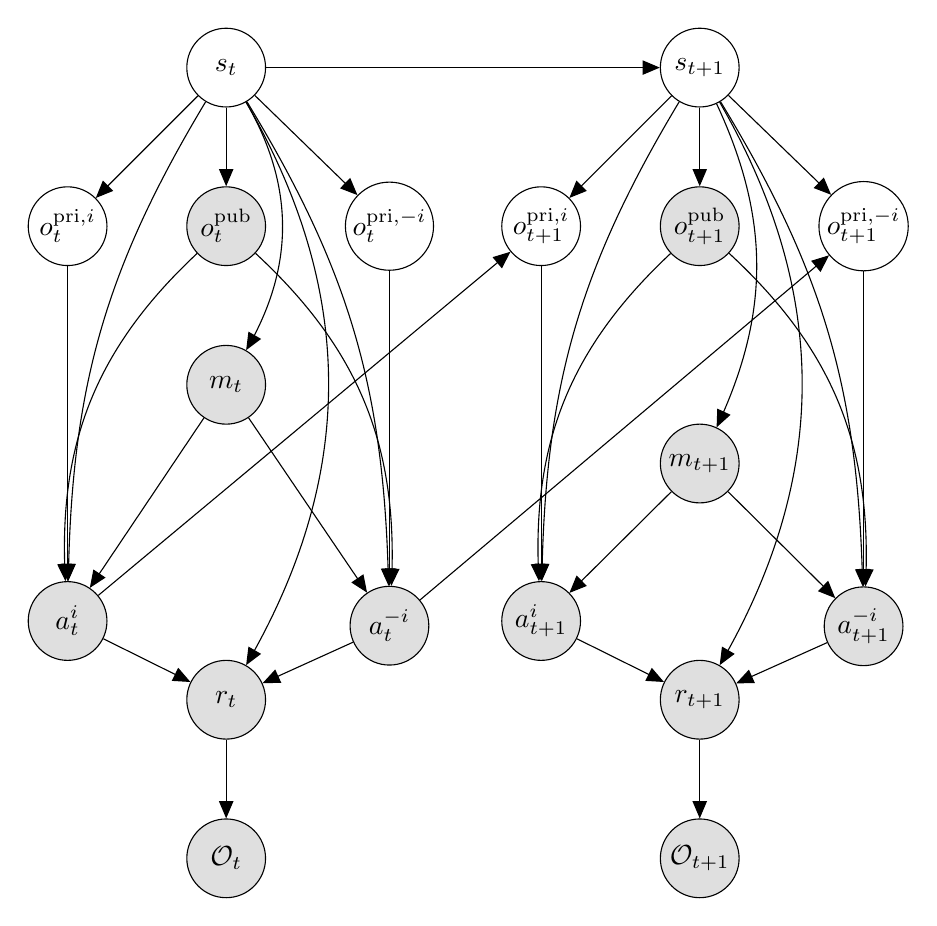
\begin{tikzpicture}[latent/.append style={minimum size=1.0cm}]
        \node[latent] (st) {$s_t$};
        \node[obs, below=of st] (o-pubt) {$o^{\operatorname{pub}}_t$};
        \node[obs, below=1cmof o-pubt] (msg) {$m_t$};
        \node[latent, left=of o-pubt] (o-pri-1t) {$o^{\operatorname{pri}, i}_t$};
        \node[latent, right=of o-pubt] (o-pri-2t) {$o^{\operatorname{pri}, -i}_t$};
        \node[obs, below=4cm of o-pri-1t] (a1t) {$a^{i}_t$};
        \node[obs, below=4cm of o-pri-2t] (a2t) {$a^{-i}_t$};
        \node[obs, below=5cm of o-pubt] (reward-t) {$r_t$};
        \node[obs, below=of reward-t] (optim-t) {$\mathcal{O}_t$};
        
        \node[latent, right=5cm of st] (st1) {$s_{t+1}$};
        \node[obs, below=of st1] (o-pubt1) {$o^{\operatorname{pub}}_{t+1}$};
        \node[obs, below=2cmof o-pubt1] (msg1) {$m_{t+1}$};
        \node[latent, left=of o-pubt1] (o-pri-1t1) {$o^{\operatorname{pri}, i}_{t+1}$};
        \node[latent, right=of o-pubt1] (o-pri-2t1) {$o^{\operatorname{pri}, -i}_{t+1}$};
        \node[obs, below=4cm of o-pri-1t1] (a1t1) {$a^{i}_{t+1}$};
        \node[obs, below=4cm of o-pri-2t1] (a2t1) {$a^{-i}_{t+1}$};
        \node[obs, below=5cm of o-pubt1] (reward-t1) {$r_{t+1}$};
        \node[obs, below=of reward-t1] (optim-t1) {$\mathcal{O}_{t+1}$};
        
        \edge {st} {o-pubt, o-pri-1t, o-pri-2t, st1}
        \edge {st1} {o-pubt1, o-pri-1t1, o-pri-2t1}
        \edge {o-pri-1t} {a1t}
        \edge {o-pri-2t} {a2t}
        
        \edge {reward-t1} {optim-t1}
        \edge {reward-t} {optim-t}
        
        \path[->]  (st)  edge   [bend right=15] node {} (a1t);
        \path[->]  (st)  edge   [bend left=15] node {} (a2t);
        \path[->]  (st)  edge   [bend left=30] node {} (msg);
        \path[->]  (st)  edge   [bend left=30] node {} (reward-t);
        \path[->]  (o-pubt)  edge   [bend right=25] node {} (a1t);
        \path[->]  (o-pubt)  edge   [bend left=25] node {} (a2t);
        
        \edge {msg} {a1t, a2t}
        
        \edge {a1t} {o-pri-1t1}
        \edge {a2t} {o-pri-2t1}
        
        \edge {a1t, a2t} {reward-t}
        \edge {o-pri-1t1} {a1t1}
        \edge {o-pri-2t1} {a2t1}
        
        \edge {a1t1, a2t1} {reward-t1}
        \path[->]  (st1)  edge   [bend right=15] node {} (a1t1);
        \path[->]  (st1)  edge   [bend left=15] node {} (a2t1);
        \path[->]  (st1)  edge   [bend left=25] node {} (msg1);
        \path[->]  (st1)  edge   [bend left=30] node {} (reward-t1);
        \path[->]  (o-pubt1)  edge   [bend right=25] node {} (a1t1);
        \path[->]  (o-pubt1)  edge   [bend left=25] node {} (a2t1);
        \edge {msg1} {a1t1, a2t1}
    \end{tikzpicture}
    \end{minipage}%
    \begin{minipage}[t]{0.5\linewidth}
    \caption{The graphical model represents the public belief POMDP $o^{\operatorname{pub}}$ representing the public observation, which depends on the current state and agents' action. We left the state transition function $P(s_{t+1} | s_t, a_t)$ to reduce the clusters. We assume a cooperative setting in which each agent (including the public belief agent) trying to optimize}
    \label{fig:chap4-public-belief-MARL}
    \end{minipage}
\end{figure}
The reason we split between reward $r_t$ and optimality $\mathcal{O}_t$ is that the reward will depend on unknown state hence but when we are training agent we didn't know that state. This separation will be clear after we have derived the public agent. Let's start by defining our joint distribution for this:
\begin{equation}
\label{eqn:elbo-pub-belief}
\begin{aligned}
    P(s_0)  \prod^T_{t=0} &P(s_{t+1} | s_t, a_t^i, a_t^{-i}) P(o^{\pri, i}_{t+1} | s_{t+1}, a^i_t) P(o^{\pri, -i}_{t+1} | s_{t+1}, a^{-i}_t) P(o^{\pub}_{t+1} | s_{t+1}, a^i_t, a^{-i}_t) \\
    &P(a^i_t | s_t, o^{\pri, i}_t, m_t, o^{\pub}_t) P(a^{-i}_t | s_t, o^{\pri, -i}_t, m_t, o^{\pub}_t) P(\mathcal{O}_t| r_t) P(r_t | s_t, a^i_t, a^{-i}_t) P(m_t | s_t)
\end{aligned}
\end{equation}
Let's consider the following scenario: In card games, usually, the public observation consists of action of agents and possibly a public card. The action of agents can also affect the state. The state is the configuration of the cards for all players, and the private observation process $P(o^{\pri, i}_{t+1} | s_{t+1}, a^i_t)$ is simply a mask to the state that allows us to see only our card, a similar process occurs with the public card $P(o^{\pub}_{t+1} | s_{t+1}, a^i_t, a^{-i}_t)$. This shows that the state is sufficiently statistic for individual private observation. Now, it's the time to consider the derivation of a public agent, which we can treat as POMDP problem, where the derivation follows \cite{shvechikovjoint}. We consider the variational distribution for the public agent:
\begin{equation}
\begin{aligned}
    P(s_0) &\bracka{\prod^T_{t=0} q(s_{t+1} | s_t, a^i_t, a^{-i}_t, o^{\pub}_{t+1}, m_t, \mathcal{O}_t, r_t)}\bracka{\prod^T_{t=0}q( o^{\pri, i}_{t+1}| s_t, a^i_t, o^{\pub}_{t+1}, m_t, \mathcal{O}_t, r_t)} \\
    &\bracka{\prod^T_{t=0}q(o^{\pri, -i}_{t+1} | s_t, a^{-i}_t, o^{\pub}_{t+1}, m_t, \mathcal{O}_t, r_t)}\bracka{\prod^T_{t=0} q(m_t | o^{\pub}_{1:t}, a^{i}_{1:t}, a^{-i}_{1:t}, \mathcal{O}_{1:T}, r_{1:T})}
\end{aligned}
\end{equation} 
Let's consider the ELBO for the problem. We have the following:
\begin{equation}
\begin{aligned}
    \mathbb{E}\Bigg[ \sum^T_{t=1} \log &\frac{ P(s_{t+1} | s_t, a_t^i, a_t^{-i})P(o^{\pri, i}_{t+1} | s_{t+1}, a^i_t) P(o^{\pri, -i}_{t+1} | s_{t+1}, a^{-i}_t) P(o^{\pub}_{t+1} | s_{t+1}, a^i_t, a^{-i}_t) P(a^i_t | s_t, o^{\pri, i}_t, m_t, o^{\pub}_t)  }{q(s_{t+1}, o^{\pri, i}_{t+1}, o^{\pri, -i}_{t+1} | s_t, a^i_t, a^{-i}_t, o^{\pub}_{t+1}, m_t, \mathcal{O}_t, r_t)} \\
    &\cdot \frac{P(m_t | s_t) P(\mathcal{O}_t, r_t | r_t)P(r_t | s_t, a^i_t, a^{-i}_t) P(a^{-i}_t | s_t, o^{\pri, -i}_t, m_t, o^{\pub}_t)}{q(m_t | o^{\pub}_{1:t}, a^{i}_{1:t}, a^{-i}_{1:t}, \mathcal{O}_{1:T}, r_{1:T})}  \Bigg]
\end{aligned}
\end{equation}
Now, we want to infer the unknown given what we can observe:
\begin{equation}
\begin{aligned}
    P(s_{t+1}, o^{\pri, i}_{t+1}, &o^{\pri, -i}_{t+1}, m_t | a^{i}_{1:t}, a^{-i}_{1:t}, \mathcal{O}_{1:T}, r_{1:T}, o^{\pub}_{1:t+1}) \\
    &= \frac{P(s_{t+1}, o^{\pri, i}_{t+1}, o^{\pri, -i}_{t+1}, m_t, a^i_t, a^{-i}_t, \mathcal{O}_t, r_t , o^{\pub}_{t+1}| a^{i}_{1:t-1}, a^{-i}_{1:t-1}, \mathcal{O}_{1:t-1}, r_{1:t-1}, o^{\pub}_{1:t})}{P(a^i_t, a^{-i}_t, \mathcal{O}_t, r_t, o^{\pub}_{t+1} | a^{i}_{1:t-1}, a^{-i}_{1:t-1}, \mathcal{O}_{1:t-1}, r_{1:t-1}, o^{\pub}_{1:t})}
\end{aligned}
\end{equation}
We shall consider the numerator first, since we can see that the current is conditional independent given the current state.
\begin{equation}
\begin{aligned}
    P(s_{t+1}, &o^{\pri, i}_{t+1}, o^{\pri, -i}_{t+1}, m_t, a^i_t, a^{-i}_t, \mathcal{O}_t, r_t , o^{\pub}_{t+1}| a^{i}_{1:t-1}, a^{-i}_{1:t-1}, \mathcal{O}_{1:t-1}, r_{1:t-1}, o^{\pub}_{1:t}) \\
    &= \int P(s_{t+1}, o^{\pri, i}_{t+1}, o^{\pri, -i}_{t+1}, m_t, a^i_t, a^{-i}_t, \mathcal{O}_t, r_t , o^{\pub}_{t+1} | s_t) 
    P(s_t | a^{i}_{1:t-1}, a^{-i}_{1:t-1}, \mathcal{O}_{1:t-1}, r_{1:t-1}, o^{\pub}_{1:t}) \dby s_t
\end{aligned}
\end{equation}
Let's perform the importance sampling using the proposal distribution or the variational distribution:
\begin{equation}
\begin{aligned}
    \int P(s_{t+1}, &o^{\pri, i}_{t+1}, o^{\pri, -i}_{t+1}, m_t, a^i_t, a^{-i}_t, \mathcal{O}_t, r_t , o^{\pub}_{t+1} | s_t) 
    P(s_t | a^{i}_{1:t-1}, a^{-i}_{1:t-1}, \mathcal{O}_{1:t-1}, r_{1:t-1}, o^{\pub}_{1:t})\dby s_t \\
    &= \begin{aligned}[t]
        \int \frac{P(s_{t+1}, o^{\pri, i}_{t+1}, o^{\pri, -i}_{t+1}, m_t, a^i_t, a^{-i}_t, \mathcal{O}_t, r_t , o^{\pub}_{t+1} | s_t)}{q(s_{t+1}, o^{\pri, i}_{t+1}, o^{\pri, -i}_{t+1}, m_t)} &q(s_{t+1}, o^{\pri, i}_{t+1}, o^{\pri, -i}_{t+1}, m_t) \\
        &P(s_t | a^{i}_{1:t-1}, a^{-i}_{1:t-1}, \mathcal{O}_{1:t-1}, r_{1:t-1}, o^{\pub}_{1:t}) \dby s_t
    \end{aligned}
\end{aligned}
\end{equation}
We will denote the importance weight $w_{t+1}(s_t, s_{t+1}, o^{\pri, i}_{t+1}, o^{\pri, -i}_{t+1}, m_t)$ as 
\begin{equation}
    w_{t+1}(s_t, s_{t+1}, o^{\pri, i}_{t+1}, o^{\pri, -i}_{t+1}, m_t) = \frac{P(s_{t+1}, o^{\pri, i}_{t+1}, o^{\pri, -i}_{t+1}, m_t, a^i_t, a^{-i}_t, \mathcal{O}_t, r_t , o^{\pub}_{t+1} | s_t)}{q(s_{t+1}, o^{\pri, i}_{t+1}, o^{\pri, -i}_{t+1}, m_t)}
\end{equation}
Now given the following importance sampling, we can see that we can sample the state $s_t$ by using ancestor index $u^k_t$. Let's approximate this using ancestor index type sampling:
\begin{equation}
\label{eqn:chap5-sample-index}
\begin{aligned}
    &\frac{1}{K}\sum^K_{k=1} w_{t+1}(s_t^{u^k_t}, s_{t+1}, o^{\pri, i}_{t+1}, o^{\pri, -i}_{t+1}, m_t) \cdot q(s_{t+1}, o^{\pri, i}_{t+1}, o^{\pri, -i}_{t+1}, m_t | s_t^{u^k_t}, a^i_t, a^{-i}_t, o^{\pub}_{t+1}) \\
    =&\begin{aligned}[t]
        \frac{1}{K}\sum^K_{k=1} w_{t+1}(s_t^{u^k_t}, s_{t+1}, o^{\pri, i}_{t+1}, o^{\pri, -i}_{t+1}, m_t) &q(s_{t+1} | s_t^{u^k_t}, a^i_t, a^{-i}_t, o^{\pub}_{t+1}) q(o^{\pri, i}_{t+1} | s_t^{u^k_t}, a^i_t, m_t, \mathcal{O}_{1:T}, r_{1:T}, o^{\pub}_{t+1}) \\
        &q(o^{\pri, -i}_{t+1} | s_t^{u^k_t}, a^{-i}_t, m_t, \mathcal{O}_{1:T}, r_{1:T}, o^{\pub}_{t+1})  q(m_t | o^{\pub}_{1:t}, a^{-i}_{1:t}, a^i_{1:t}, \mathcal{O}_{1:T}, r_{1:T})
    \end{aligned} \\
    \approx&\begin{aligned}[t]
        \frac{1}{K}\sum^K_{k=1} w_{t+1}(s_t^{u^k_t}, s_{t+1}^k, o^{\pri, i, k}_{t+1}, o^{\pri, -i, k}_{t+1}, m_t^1) &\delta (s_{t+1} - s_{t+1}^k) \delta (o^{\pri, i}_{t+1} - o^{\pri, i, k}_{t+1}) \\
        &\delta (o^{\pri, -i}_{t+1} - o^{\pri, -i, k}_{t+1}) \delta (m_t - m_t^1)
        % &q(s_{t+1} | s_t^{u^k_t}, a^i_t, a^{-i}_t, o^{\pub}_{t+1}) q(o^{\pri, i}_{t+1} | s_t^{u^k_t}, a^i_t) \\
        % &q(o^{\pri, -i}_{t+1} | s_t^{u^k_t}, a^{-i}_t)  q(m_t | o^{\pub}_{1:t}, \mathcal{O}_{1:T}, r_{1:T})
    \end{aligned} \\
\end{aligned}
\end{equation}
We can see above that we can further approximate our equation using sampling from our proposal/variational distribution. Now, we can fine the denominator by marginalization. Given this we have the final posterior being weighted mixture of particles:
\begin{equation}
\begin{aligned}
    P(s_{t+1},& o^{\pri, i}_{t+1}, o^{\pri, -i}_{t+1}, m_t | a^{i}_{1:t}, a^{-i}_{1:t}, \mathcal{O}_{1:T}, r_{1:T}, o^{\pub}_{1:t+1}) \\
    &=\frac{1}{K}\sum^K_{k=1} W^k_{t+1} \delta (s_{t+1} - s_{t+1}^k) \delta (o^{\pri, i}_{t+1} - o^{\pri, i, k}_{t+1}) \delta (o^{\pri, -i}_{t+1} - o^{\pri, -i, k}_{t+1}) \delta (m_t - m_t^1)
\end{aligned}
\end{equation}
where the $W^k_{t+1}$ is the re-normalized weight. Now, the probability over the state is simply:
\begin{equation}
    P(s_{t+1} | a^{i}_{1:t}, a^{-i}_{1:t}, \mathcal{O}_{1:T}, r_{1:T}, o^{\pub}_{1:t+1}) = \frac{1}{K}\sum^K_{k=1} W^k_{t+1} \delta (s_{t+1} - s_{t+1}^k)
\end{equation}
which we can sample future state using ancestor index similar to equation \ref{eqn:chap5-sample-index}. Now, since the probability of the observable variable is:
\begin{equation}
    P(a^{i}_{1:\tau}, a^{-i}_{1:\tau}, \mathcal{O}_{1:\tau}, r_{1:\tau} o^{\pub}_{1:\tau}) = \prod^\tau_{t=0}\frac{1}{K}\sum^K_{k=1} w_{t+1}(s_t^{u^k_t}, s_{t+1}^k, o^{\pri, i, k}_{t+1}, o^{\pri, -i, k}_{t+1}, m_t^1)
\end{equation}
which is a tighter variational lower bound. Now, the objective becomes:
\begin{equation}
    \mathbb{E}\brackb{\sum^\tau_{t=0} \log \frac{1}{K} \sum ^K_{k=1} w_{t+1}(s_t^{u^k_t}, s_{t+1}^k, o^{\pri, i, k}_{t+1}, o^{\pri, -i, k}_{t+1}, m_t^1)}
\end{equation}
Let's recall the definition of the importance weight with suitable indexes:
\begin{equation}
\begin{aligned}
    &\frac{P(s_{t+1}^k | s_t^{u^k_t}, a_t^i, a_t^{-i})P(o^{\pri, i, k}_{t+1} | s_{t+1}^k, a^i_t) P(o^{\pri, -i, k}_{t+1} | s_{t+1}^k, a^{-i}_t) P(o^{\pub}_{t+1} | s_{t+1}^k, a^i_t, a^{-i}_t)}{q(s_{t+1}^k | s_t^{u^k_t}, a^i_t, a^{-i}_t, o^{\pub}_{t+1}, m_t, \mathcal{O}_t, r_t)} \\
    \times&\frac{P(a^i_t, a^{-i}_t | s_t^{u^k_t}, o^{\pri, i}_t, o^{\pri, -i}_t, m_t, o^{\pub}_t) P(m_t | s_t^{u^k_t}) P(\mathcal{O}_t | r_t)}{q(o^{\pri, i, k}_{t+1}, o^{\pri, -i, k}_{t+1} | s_t^{u^k_t}, a^i_t, a^{-i}_t, m_t, o^{\pub}_{t+1}, \mathcal{O}_t, r_t)} \\
    \times&\frac{P(\mathcal{O}_t | r_t)}{q(m_t | o^{\pub}_{1:t}, a^{i}_{1:t}, a^{-i}_{1:t}, \mathcal{O}_{1:T}, r_{1:T})}
\end{aligned}
\end{equation}
We have the following objective that follows maximum entropy framework:
\begin{equation}
\begin{aligned}
\label{eqn:chap5-elbo-public-agent}
    \mathbb{E}\Bigg[\sum^\tau_{t=0} &\log P(\mathcal{O}_t | r_t) + \mathbb{H}\brackb{q(m_t | o^{\pub}_{1:t}, a^{i}_{1:t}, a^{-i}_{1:t}, \mathcal{O}_{1:T}, r_{1:T})} \\
    &+ \log \frac{1}{K} \sum ^K_{k=1}\Bigg(\frac{P(s_{t+1}^k | s_t^{u^k_t}, a_t^i, a_t^{-i})P(o^{\pri, i, k}_{t+1} | s_{t+1}^k, a^i_t) P(o^{\pri, -i, k}_{t+1} | s_{t+1}^k, a^{-i}_t) P(o^{\pub}_{t+1} | s_{t+1}^k, a^i_t, a^{-i}_t)}{q(s_{t+1}^k | s_t^{u^k_t}, a^i_t, a^{-i}_t, o^{\pub}_{t+1}, m_t, \mathcal{O}_t, r_t)} \\
    &\cdot \frac{P(a^i_t, a^{-i}_t | s_t^{u^k_t}, o^{\pri, i, k}_t, o^{\pri, -i, k}_t, m_t, o^{\pub}_t) P(m_t | s_t^{u^k_t}) P(\mathcal{O}_t | r_t)}{q(o^{\pri, i, k}_{t+1}, o^{\pri, -i, k}_{t+1} | s_t^{u^k_t}, a^i_t, a^{-i}_t, m_t, o^{\pub}_{t+1}, \mathcal{O}_t, r_t)} \Bigg)\Bigg]
\end{aligned}
\end{equation}
Now, in practice the public agent shall be a weighted sum of underlying state, public observation, and agent actions i.e
\begin{equation}
    \sum^K_{k=1} W^k_t \pi(m^k_t | s^k_t, o^{\pub}_t, a^i_t, a^{-i}_t)
\end{equation}
There are two minor issues that we want to consider (that we have mentioned above):
\begin{itemize}
    \item The interpretability of $o^{\pri, i, k}_t$ and $o^{\pri, -i, k}_t$. There isn't a lot we can do with this apart from constructing a network that would translate the public agent's private observation into the agent's private observation. Or we can pretrain a network that output the agents' private observation. However, we have to make sure not to change the main public agent's network by backpropagating the local feature, since all the agents must have the same public agent.
    \item The joint action $P(a^i_t, a^{-i}_t | s_t^{u^k_t}, o^{\pri, i}_t, o^{\pri, -i}_t, m_t, o^{\pub}_t)$. After having all the private observation and public observation, we can try to optimize the reconstruction loss on the agents' actions. However, we can further assume that the agents' policies are based on Boltzmann distribution of action-value function. Given this assumption, the maximum-log-likelihood estimation should follow the usual adversarial imitation learning that we have extensively discussed in \cite{finn2016connection, yu2019multi}. For a normal scenario, we simply able to train its action function. As noted before, we shouldn't include any additional information from the agent to help us with the public agent (including the agent's action-value function). 
\end{itemize}
We would like to state that all the problems above can be lifted if we assume that each agent has its own public agent and trying to model others using oneself or other methods. By ignoring the common knowledge of messages $m_t$, we lose a guarantee that the agents will be in "sync" of each other, thus returning to a problem of equilibrium selection. Finally, we shall consider the individual agent that corresponds on the message, its private observation, and the state. Let's start with the definition of action-value function $Q(s_t, a^i_t, m_t, o^{\pri, i}_t, o^{\pub}_t)$, which is defined as:
\begin{equation}
    Q(\{s_t\}^K_{k=1}, a^i_t, m_t, o^{\pri, i}_t, o^{\pub}_t) = \sum^K_{k=1} W^k_t Q(s_t^k, a^i_t, m_t, o^{\pri, i}_t, o^{\pub}_t)
\end{equation}
The agent is based on single agent problem, which we can find its policy as:
\begin{equation}
\begin{aligned}
    &\pi(a^i_t | \{s_t^k\}^K_{k=1}, m_t, o^{\pri, i}_t, o^{\pub}_t) = \frac{P_\prior(a^i_t | \{s_t^k\}^K_{k=1}, m_t, o^{\pri, i}_t, o^{\pub}_t)\exp{Q(\{s_t^k\}^K_{k=1}, a^i_t, m_t, o^{\pri, i}_t, o^{\pub}_t)}}{V(\{s_t^k\}^K_{k=1}, m_t, o^{\pri, i}_t, o^{\pub}_t)} \\
    \text{ where }&Q(s_t, a^i_t, m_t, o^{\pri, i}_t, o^{\pub}_t) = r_t + \gamma\mathbb{E}\brackb{Q(\{s_{t+1}^k\}^K_{k=1}, m_{t+1}, o^{\pri, i}_{t+1}, o^{\pub}_{t+1})} \\
    &V(\{s_t^k\}^K_{k=1}, m_t, o^{\pri, i}_t, o^{\pub}_t) = \int P_\prior(a^i_t | \{s_t^k\}^K_{k=1}, m_t, o^{\pri, i}_t, o^{\pub}_t)\exp{Q(\{s_t^k\}^K_{k=1}, a^i_t, m_t, o^{\pri, i}_t, o^{\pub}_t)} \dby a^i_t
\end{aligned}
\end{equation}
% while the final policy is a weighted sum of all possible states
% \begin{equation}
%     \sum^K_{k=1} W^k_t \pi(a^i_t | s_t^k, m_t, o^{\pri, i}_t, o^{\pub}_t)
% \end{equation}
% This concludes the derivation of the policy and we will consider the implementation of public agent agent and lower level policy.

\section{Implementation}
\label{sec:chap5-public-agent-implementation}
Now, let's consider the implementation of public agent, which is similar to DVRL. Starting with the hidden state calculation for each time step, we have 3 hidden variables that we have to infer
\begin{equation}
\begin{aligned}
    &u^k_{t-1} \sim \text{Categorical}\bracka{\frac{w^k_{t-1}}{\sum^K_{k=1}w^k_{t-1}}} \\
    &x^k_{t+1} \sim q_\psi(s_{t+1} | f^{u^k_t}_t, a^i_t, a^{-i}_t, o^{\pub}_{t+1}, m_t, r_t) \\
    &y^k_{t+1} \sim q_\psi(o^{\pri, i}_{t+1} | f^{u^k_t}_t, a^i_t, o^{\pub}_{t+1}, m_t, r_t) \\ 
    &z^k_{t+1} \sim q_\psi(o^{\pri, -i}_{t+1} | f^{u^k_t}_t, a^{-i}_t, o^{\pub}_{t+1}, m_t, r_t) \\
    &f^k_t = \psi^{\text{RNN} \ 1}_\theta (x^k_{t+1}, f^{u^k_t}_t, a^i_t, a^{-i}_t, o^{\pub}_{t+1}, m_t, \mathcal{O}_t, r_t) \\
    &g^k_t = \psi^{\text{RNN} \ 2}_\theta (y^k_{t+1}, g^{u^k_t}_t, a^i_t, o^{\pub}_{t+1}, m_t, r_t) \\
    &h^k_t = \psi^{\text{RNN} \ 3}_\theta (z^k_{t+1}, h^{u^k_t}_t, a^{-i}_t, o^{\pub}_{t+1}, m_t, r_t) \\
    &w^k_T = \begin{aligned}[t]
        &\frac{P_\theta(s_{t+1}^k | s_t^{u^k_t}, a_t^i, a_t^{-i})P_\theta(o^{\pri, i, k}_{t+1} | s_{t+1}^k, a^i_t) P_\theta(o^{\pri, -i, k}_{t+1} | s_{t+1}^k, a^{-i}_t) P_\theta(o^{\pub}_{t+1} | s_{t+1}^k, a^i_t, a^{-i}_t)}{q_\psi(s_{t+1}^k | s_t^{u^k_t}, a^i_t, a^{-i}_t, o^{\pub}_{t+1}, m_t, r_t)} \\
        \cdot&\frac{P_\theta(a^i_t, a^{-i}_t | s_t^{u^k_t}, o^{\pri, i}_t, o^{\pri, -i}_t, m_t, o^{\pub}_t) P_\theta(m_t | s_t^{u^k_t}) P_\theta(\mathcal{O}_t | r_t)}{q_\psi(o^{\pri, i, k}_{t+1}, o^{\pri, -i, k}_{t+1} | s_t^{u^k_t}, a^i_t, a^{-i}_t, m_t, o^{\pub}_{t+1}, r_t)} \cdot \frac{P_\theta(\mathcal{O}_t | r_t)}{q_\psi(m_t | o^{\pub}_{1:t}, a^{i}_{1:t}, a^{-i}_{1:t}, r_{1:T})}
    \end{aligned}
\end{aligned}
\end{equation}
Now, we have the following particles, which is in tuple $(x^k_{t+1}, y^k_{t+1}, z^k_{t+1}, f^k_t, g^k_t, h^k_t, w^k_t)$. Now the agent have to be optimized the EBLO in equation \ref{eqn:chap5-elbo-public-agent}, where we have 
\begin{equation}
\begin{aligned}
\label{eqn:chap5-elbo-public-agent}
    \mathbb{E}\Bigg[\sum^\tau_{t=0} &\log P(\mathcal{O}_t | r_t) + \mathbb{H}\brackb{q_\psi(m_t | o^{\pub}_{1:t}, a^{i}_{1:t}, a^{-i}_{1:t}, \mathcal{O}_{1:T}, r_{1:T})} + \log \frac{1}{K} \sum ^K_{k=1}\tilde{w}_t^k\Bigg]
\end{aligned}
\end{equation}
where 
\begin{equation}
\begin{aligned}
    \tilde{w}_t^k = &\frac{P_\theta(s_{t+1}^k | s_t^{u^k_t}, a_t^i, a_t^{-i})P_\theta(o^{\pri, i, k}_{t+1} | s_{t+1}^k, a^i_t) P_\theta(o^{\pri, -i, k}_{t+1} | s_{t+1}^k, a^{-i}_t) P_\theta(o^{\pub}_{t+1} | s_{t+1}^k, a^i_t, a^{-i}_t)}{q_\psi(s_{t+1}^k | s_t^{u^k_t}, a^i_t, a^{-i}_t, o^{\pub}_{t+1}, m_t, \mathcal{O}_t, r_t)} \\
    &\cdot \frac{P_\theta(a^i_t, a^{-i}_t | s_t^{u^k_t}, o^{\pri, i, k}_t, o^{\pri, -i, k}_t, m_t, o^{\pub}_t) P_\theta(m_t | s_t^{u^k_t}) P_\theta(\mathcal{O}_t | r_t)}{q_\psi(o^{\pri, i, k}_{t+1}, o^{\pri, -i, k}_{t+1} | s_t^{u^k_t}, a^i_t, a^{-i}_t, m_t, o^{\pub}_{t+1}, \mathcal{O}_t, r_t)} 
\end{aligned}
\end{equation}
Now, let's consider the lower agent objective. We are going to start with the definition of the value function $V(\{s_t^k\}^K_{k=1}, m_t, o^{\pri, i}_t, o^{\pub}_t)$, which trained to minimize:
\begin{equation}
\begin{aligned}
\mathcal{L}_{V} = \mathbb{E}_{\{s_t^k\}^K_{k=1}, m_t, o^{\pri, i}_t, o^{\pub}_t\sim \mathcal{D}} \Bigg[\frac{1}{2}\Bigg(&V(\{s_t^k\}^K_{k=1}, m_t, o^{\pri, i}_t, o^{\pub}_t) \\
&- \mathbb{E}_{a_t^i}\brackb{q_\psi(\{s_t^k\}^K_{k=1}, a^i_t, m_t, o^{\pri, i}_t, o^{\pub}_t) - \log \frac{P_\prior(a^i_t | \{s_t^k\}^K_{k=1}, m_t, o^{\pri, i}_t, o^{\pub}_t)}{\pi(a^i_t | \{s_t^k\}^K_{k=1}, m_t, o^{\pri, i}_t, o^{\pub}_t)}}\Bigg)^2\Bigg]
\end{aligned}
\end{equation}
where the action is sampled from $a^i_t \sim \pi(a^i_t | \{s_t^k\}^K_{k=1}, m_t, o^{\pri, i}_t, o^{\pub}_t)$. Now for the action value function, we follows from the Bellman equation:
\begin{equation}
\begin{aligned}
    \mathcal{L}_Q = \mathbb{E}_{\{s_t^k\}^K_{k=1}, m_t, o^{\pri, i}_t, o^{\pub}_t, r_t, \{s_{t+1}^k\}^K_{k=1},m_{t+1}, o^{\pri, i}_{t+1}, o^{\pub}_{t+1},\sim \mathcal{D}}\Bigg[\frac{1}{2}\Bigg( &q_\psi(\{s_t^k\}^K_{k=1}, a^i_t, m_t, o^{\pri, i}_t, o^{\pub}_t)  \\
    &- \brackb{r_t + \gamma V(\{s_{t+1}^k\}^K_{k=1}, m_{t+1}, o^{\pri, i}_{t+1}, o^{\pub}_{t+1})} \Bigg)\Bigg]
\end{aligned}
\end{equation}
Finally, the policy will be in the form of $f(\xi ; \{s_t^k\}^K_{k=1}, m_t, o^{\pri, i}_t, o^{\pub}_t)$ where $\xi \sim \mathcal{N}(0, I)$ and trained using minimizing the KL-divergence:
\begin{equation}
    \loss_{\pi} = \kl\bracka{\pi(a^i_t | \{s_t^k\}^K_{k=1}, m_t, o^{\pri, i}_t, o^{\pub}_t)\Bigg\|\frac{P_\prior(a^i_t | \{s_t^k\}^K_{k=1}, m_t, o^{\pri, i}_t, o^{\pub}_t)\exp{q_\psi(\{s_t^k\}^K_{k=1}, a^i_t, m_t, o^{\pri, i}_t, o^{\pub}_t)}}{V(\{s_t^k\}^K_{k=1}, m_t, o^{\pri, i}_t, o^{\pub}_t)}}
\end{equation}
Given this, we conclude the training for probabilistic public-agent.
    



\chapter{Hierarchy and Communication in Multi-Agent Reinforcement Learning}
\label{chapter:chap6}
\begin{miniabstract}
After we have a unified view on MAPI framework, which we have reinterpret Balancing Q-learning \cite{grau2018balancing} as a probabilistic inference. We are now going to consider extensions to agent's functionality. In this chapter, we are going to consider the case of temporal abstraction and communication in coopeartive multi-agent reinforcement learning problem. We will start by considering single agent option learning problem and solving it together with soft actor-critic like algorithm, as a minor contribution. After considering single agent problem, we are going to define a model in which the agent can plan and communicate and solving then.
\end{miniabstract}


\section{Single Agent Soft-Hierarchical Reinforcement Learning}
\label{sec:chap4-single-soft-HRL}
We will associate our model with option learning paradigm, and extends the result in \cite{igl2019multitask} by cooperating Soft-Actor Critic type solution as it is standard method for solving probabilistic reinforcement learning. Furthermore, our approach is similar to \cite{daniel2016probabilistic}, in terms of using similar probabilistic technique, however, in the paper, the authors concerning more on inferring policies from expert data, while didn't explicitly solve for each policy given the optimally condition (what we are trying to do now). In the nutshell, we have a master policy $\pi^H$ that suggesting the "mode of execution" or option to lower level policy $\pi$ based on termination policy $\pi^T$, which telling what the next option should be. The joint distribution of actions i.e $P(s_{1:T}, a_{1:T}, \mathcal{O}_{1:T}, z_{1:T}, b_{1:T})$ is depicted in figure \ref{fig:chap4-single-agent-hierarchical}.
\begin{figure}[ht]
    \begin{minipage}[t]{0.5\linewidth}
    \centering
    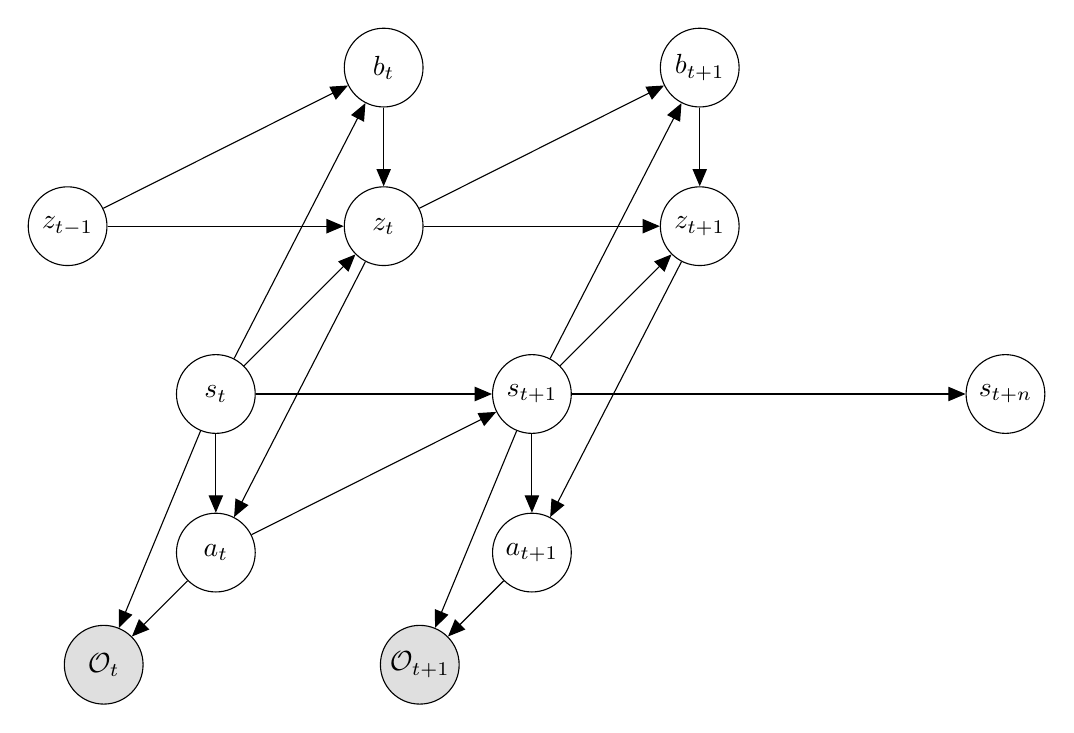
\begin{tikzpicture}[latent/.append style={minimum size=1.0cm}]
        \node[latent] (st) {$s_t$};
        \node[latent, below=of st] (at) {$a_t$};
        \node[latent, above right=2cm of st] (zt) {$z_t$};
        \node[latent, above=of zt] (bt) {$b_t$};
        \node[obs, below left=of at] (ot) {$\mathcal{O}_t$};
        
        \node[latent, left=3cm of zt] (zt-1) {$z_{t-1}$};
        
        % \edge{o1t} {a1t}
        \edge {st} {at, zt, bt}
        \edge {bt} {zt}
        \edge {zt}  {at}
        \edge {zt-1}  {bt, zt}
        \edge {at, st} {ot}
    
        \node[latent, right=3cmof st] (st1) {$s_{t+1}$};
        \node[latent, below=of st1] (at1) {$a_{t+1}$};
        \node[latent, above right=2cm of st1] (zt1) {$z_{t+1}$};
        \node[latent, above=of zt1] (bt1) {$b_{t+1}$};
        \node[obs, below left=of at1] (ot1) {$\mathcal{O}_{t+1}$};
        
        \edge {st, at} {st1}
        
        \edge {st1} {at1, zt1, bt1}
        \edge {bt1} {zt1}
        \edge {zt1}  {at1}
        \edge {zt}  {bt1, zt1}
        \edge {at1, st1} {ot1}
        
        \node[latent, right=5cm of st1] (stn) {$s_{t+n}$};
        \path[->]  (st1)  edge [] node {} (stn);
    \end{tikzpicture}
    \end{minipage}%
    \begin{minipage}[t]{0.5\linewidth}
    \caption{The the graphical model of hierarchical agent. We have the master policy which produces $z_t$ while having switch goal policy producing policy $b_t$}
    \label{fig:chap4-single-agent-hierarchical}
    \end{minipage}
\end{figure}
The joint distribution is then 
\begin{equation}
\begin{aligned}
    P(s_{1:T}, a_{1:T}, z_{1:T}, b_{1:T}) = P(s_0)P(z_0)\prod^T_{t=0} &P(s_{t+1} | s_t, a_t) P_\prior(a_t | s_t, z_t)\\
    &P_\prior^H(z_t | s_t, z_{t-1}, b_t) P_\prior^T(b_t | s_t, z_{t-1}) P(\mathcal{O}_t = 1 | s_t, a_t)
 \end{aligned}
\end{equation}
The variations joint distribution is defined as 
\begin{equation}
\begin{aligned}
    q(s_{1:T}, a_{1:T}, z_{1:T}, b_{1:T}) = P(s_0)P(z_0)\prod^T_{t=0} &P(s_{t+1} | s_t, a_t) \pi_{\theta}(a_t | s_t, z_t)\\
    &\pi^H_{\phi}(z_t | s_t, z_{t-1}, b_t) \pi^T_{\phi}(b_t | s_t, z_{t-1}) 
\end{aligned}
\end{equation}
Usually, the master policy and its prior are defined as. 
\begin{equation}
\begin{aligned}
    &\pi^H_{\phi}(z_t | s_t, z_{t-1}, b_t) = (1-b_t) \delta(z_t  - z_{t-1}) + b_t q^H_{\phi}(z_t | s_t) \\ 
    &P_\prior^H(z_t | s_t, z_{t-1}, b_t) = (1-b_t) \delta(z_t  - z_{t-1}) + b_t \frac{1}{m}
\end{aligned}
\end{equation}
As it takes the value of $b_t$ to suggest when to change the option $z_t$. Now, the ELBO is equal to 
\begin{equation}
    \mathbb{E}\brackb{\sum^T_{t=1} \beta r(s_t, a_t) - \log \frac{\pi_{\theta}(a_t | s_t, z_t)}{P_\prior(a_t | s_t, z_t)}  - \log \frac{\pi^H_{\phi}(z_t | s_t, z_{t-1}, b_t)}{P_\prior^H(z_t | s_t, z_{t-1}, b_t)} - \log \frac{\pi^T_{\phi}(b_t | s_t, z_{t-1}) }{P_\prior^T(b_t | s_t, z_{t-1})}}
\end{equation}
This is the same as one defined in \cite{igl2019multitask}. Given the ELBO, we will consider the closed-form solution of the low-level policy/master policy and termination policy. For the low-level policy, we have 
\begin{equation}
\begin{aligned}
\label{eqn:chap4-single-HRL-lower}
    &\pi_{\theta}(a_{t} | s_{t}, z_{t}) = \frac{P_\prior(a_{t} | s_{t}, z_{t})\exp\bracka{Q(s_{t}, a_{t}, z_{t})}}{\exp V(s_{t}, z_{t})} \\
    \text{ where }&V(s_{t}, z_{t}) = \log \int P_\prior(a_{t} | s_{t}, z_{t})\exp\bracka{Q(s_{t}, a_{t}, z_{t})} \dby a_{t}
\end{aligned}
\end{equation}
For the high-level policy, we have 
\begin{equation}
\begin{aligned}
\label{eqn:chap4-single-HRL-higher}
    &\pi^H(z_t | s_t) = \frac{\frac{1}{m}\exp\bracka{Q(s_t, z_t)}}{\exp\bracka{V(s_t)}}
    \\
    \text{ where } &Q(s_t, z_t) =  V(s_t, z_t)  \\
    &V^H(s_t) =  \frac{1}{m}\log \int \exp\bracka{Q(s_t, z_t)} \dby z_T
\end{aligned} 
\end{equation}
Finally, the termination policy is  
\begin{equation}
\begin{aligned}
\label{eqn:chap4-single-HRL-termination}
    &\pi^T(b_{t} | s_{t}, z_{t-1}) = \frac{P_\prior^T(b_{t} | s_{t}, z_{t-1})\exp{V(s_{t}, z_{t-1}, b_{t})}}{\exp V(s_{t}, z_{t-1})} \\
    \text{ where }& V(s_{t}, z_{t-1}, b_{t}) = b_{t} \brackb{V^H(s_{t})} + (1-b_{t})V(s_{t}, z_{t-1}) \\
    & V(s_{t}, z_{t-1}) = \log \int P_\prior^T(b_{t} | s_{t}, z_{t-1})\exp\bracka{b_{t} \brackb{V^H(s_{t})} + (1-b_{t})V(s_{t}, z_{t-1})} \dby b_{t}
\end{aligned}
\end{equation}
Finally, the Bellman equation for soft-hierarchical single-agent reinforcement learning is 
\begin{equation}
\label{eqn:chap4-single-HRL-bellman}
    Q(s_t, a_t, z_t) = \beta r(s_t, a_t) + \gamma\mathbb{E}_{s_{t+1}}\brackb{V(s_{t+1}, z_t)}
\end{equation}
The proof will be in appendix \ref{appx:chap4-soft-single-HRL}. We can see that this is analogous to the option framework \cite{sutton1999between, bacon2017option}. Now, we have aware the work on similar topic \cite{lobo2019soft}, which the authors has almost the same solution as us but miss certain points on value function calculation, notably 
\begin{equation}
\begin{aligned}
Q(s_t, a_t, z_t) = \beta r(s_t, a_t) + \mathbb{E}_{s_{t+1}}\Big[\mathbb{E}_{b_{t+1} \sim P(b_{t+1} | s_{t+1}, z_t), z_{t+1}' \sim P(z_{t+1} | s_{t+1})}\Big[&(1-b_{t+1})V(s_{t+1 }, z_t)  \\
&+ b_{t+1}V(s_{t+1 }, z_t')\Big]\Big]
\end{aligned}
\end{equation}
The authors fails to consider the case in which the master policy soft-max the value function $V(s_{t+1}, z_{t+1})$ and assuming this 
\begin{equation}
    \mathbb{E}_{z_{t+1}' \sim P(z_{t+1} | s_{t+1})}\brackb{V(s_{t+1}, z_{t+1})}
\end{equation}
instead, which we can see that this misses the regularization of the policy $\pi^H_\phi$. By using the soft-max, we have implicitly include the regularization. 

\section{Multi-Agent Delayed Soft-Option Communication}
\label{sec:chap4-multi-soft-HRL-communication}
Now, we are going to consider multi-agent case in which we have to consider the other agent's option last time step, which is a type of delayed communication. This would be a direct extension to the single agent HRL problem. The graphical model can be too complex to draw we therefore going to show only the factorization of joint probabilities. Consider the following joint probability distribution of the problem:
\begin{equation}
\begin{aligned}
    P(&s_{1:T}, a^i_{1:T}, a^{-i}_{1:T}, z^i_{1:T}, z^{-i}_{1:T}, b^i_{1:T}, b^{-i}_{1:T}, \mathcal{O}^i_{1:T} = 1, \mathcal{O}^{-i}_{1:T} = 1) \\
    &= P(s_1)P(z^{-i}_0, z^i_0)\prod^T_{t=1} P(s_{t+1} | s_t, a_t^i, a_t^{-i})P_\prior(a^{-i}_t | s_t, z^i_t, a^i_t, z^{-i}_t) P^{H,-i}_\prior(z^{-i}_t | s_t, a^i_t, z^i_t, z^{-i}_{t-1}, b^i_t) \\
    &P^{T,-i}_\prior(b^{-i}_t | s_t,  z^{-i}_{t-1}, a^i_t, z^i_t) P_\prior(a^i_t | s_t, z^i_t, z^{-i}_{t-1}) P^{H,i}_\prior(z^i_t | s_t, z^{-i}_{t-1}, z^i_{t-1}, b^i_t) P^{T,i}_\prior(b^i_t | s_t, z^i_{t-1}, z^{-i}_{t-1})\\
    &P(\mathcal{O}^i_t = 1 | \mathcal{O}^{-i}_t = 1)P(\mathcal{O}^{-i}_t = 1)
\end{aligned}
\end{equation}
% \begin{itemize}
%     \item $P_\prior(a^i_t | s_t, z^i_t, a^{-i}_t, z^{-i}_t)$
%     \item $P^{H,i}_\prior(z^i_t | s_t, a^{-i}_t, z^{-i}_t)$
%     \item $P^{T,i}_\prior(b^i_t | s_t,  z^i_{t-1}, a^{-i}_t, z^{-i}_t)$
%     \item $P_\prior(a^{-i}_t | s_t, z^{-i}_t)$
%     \item $P^{H,-i}_\prior(z^{-i}_t | s_t, z^{-i}_{t-1}, b^{-i}_t)$
%     \item $P^{T,-i}_\prior(b^{-i}_t | s_t, z^{-i}_{t-1})$
% \end{itemize}
% WE HAVE
% \begin{itemize}
%     \item $P_\prior(a^{-i}_t | s_t, z^i_t, a^i_t, z^{-i}_t)$
%     \item $P^{H,-i}_\prior(z^{-i}_t | s_t, a^i_t, z^i_t, z^{-i}_{t-1}, b^i_t)$
%     \item $P^{T,-i}_\prior(b^{-i}_t | s_t,  z^{-i}_{t-1}, a^i_t, z^i_t)$
%     \item $P_\prior(a^i_t | s_t, z^i_t, z^{-i}_{t-1})$
%     \item $P^{H,i}_\prior(z^i_t | s_t, z^{-i}_{t-1}, z^i_{t-1}, b^i_t)$
%     \item $P^{T,i}_\prior(b^i_t | s_t, z^i_{t-1}, z^{-i}_{t-1})$
% \end{itemize}
Now, we shall consider the joint variational distribution. 
\begin{equation}
\begin{aligned}
    q(s_{1:T}, &a^i_{1:T}, a^{-i}_{1:T}, z^i_{1:T}, z^{-i}_{1:T}, b^i_{1:T}, b^{-i}_{1:T}, \mathcal{O}^{-i}_{1:T} = 1) \\
    &= P(s_1)P(z^{-i}_0, z^i_0)\prod^T_{t=1} q(s_{t+1} | s_t, a_t^i, a_t^{-i})\rho_\phi(a^{-i}_t | s_t, z^i_t, a^i_t, z^{-i}_t) q^{H,-i}(z^{-i}_t | s_t, a^i_t, z^i_t, z^{-i}_{t-1}, b^i_t) \\
    &q^{T,-i}(b^{-i}_t | s_t,  z^{-i}_{t-1}, a^i_t, z^i_t) \pi_\theta(a^i_t | s_t, z^i_t, z^{-i}_{t-1}) q^{H,i}(z^i_t | s_t, z^{-i}_{t-1}, z^i_{t-1}, b^i_t) q^{T,i}(b^i_t | s_t, z^i_{t-1}, z^{-i}_{t-1})\\
    &P(\mathcal{O}^i_t = 1 | \mathcal{O}^{-i}_t = 1)P(\mathcal{O}^{-i}_t = 1)
\end{aligned}
\end{equation}
Where we have the optimal random variable to be 
\begin{equation}
    P(\mathcal{O}^i_t = 1 | \mathcal{O}^{-i}_{1:T} = 1) \propto \exp\bracka{\beta r(s_t, a_t^i, a^{-i}_t)}
\end{equation}
Before we move on, let's specifically define the master policy's conditional probability and its prior:
\begin{equation}
\begin{aligned}
    &q^{H, i}(z^i_t | s_t, z^{-i}_{t-1}, z^i_{t-1}, b^i_t) = (1-b_t^i) \delta(z_t^i  - z_{t-1}^i) + b_t^i q^{H, i}_{\phi}(z_t^i | s_t, z^{-i}_{T-1}) \\
    &P_\prior(z^i_t | s_t, z^{-i}_{t-1}, z^i_{t-1}, b^i_t) = (1-b_t^i) \delta(z_t^i  - z_{t-1}^i) + b_t^i \frac{1}{m} \\
    &q^{H, -i}(z^{-i}_t | s_t, a^i_t, z^i_t, z^{-i}_{t-1}, b^i_t) = (1-b_t^{-i}) \delta(z_t^{-i}  - z_{t-1}^{-i}) + b_t^{-i} q^{H, -i}_{\phi}(z_t^{-i} | s_t, a^i_t, z^i_t) \\
    &P_\prior(z^{-i}_t | s_t, a^i_t, z^i_t, z^{-i}_{t-1}, b^i_t) = (1-b_t^{-i}) \delta(z_t^{-i}  - z_{t-1}^{-i}) + b_t^{-i} \frac{1}{m} \\
\end{aligned}
\end{equation}
Given both of them, we can derive the ELBO by finding KL-divergence, which is equal to 
\begin{equation}
\begin{aligned}
    \mathbb{E}_q\Bigg[\sum^T_{t=0}\beta r(s_t, a_t^i, a^{-i}_t) &- \log\frac{\pi_\theta(a^i_t | s_t, z^i_t, z^{-i}_{t-1})}{P_\prior(a^i_t | s_t, z^i_t, z^{-i}_{t-1})} - \log\frac{\rho_\theta(a^{-i}_t | s_t, z^i_t, a^i_t, z^{-i}_t) }{P_\prior(a^{-i}_t | s_t, z^i_t, a^i_t, z^{-i}_t)} \\
    &- \log\frac{q^{H, i}(z^i_t | s_t, z^{-i}_{t-1}, z^i_{t-1}, b^i_t)}{P^{H, i}_\prior(z^i_t | s_t, z^{-i}_{t-1}, z^i_{t-1}, b^i_t)} - \log\frac{q^{H, -i}(z^{-i}_t | s_t, a^i_t, z^i_t, z^{-i}_{t-1}, b^i_t)}{P^{H, -i}_\prior(z^{-i}_t | s_t, a^i_t, z^i_t, z^{-i}_{t-1}, b^i_t)} \\
    &- \log\frac{q^{T,i}(b^i_t | s_t, z^i_{t-1}, z^{-i}_{t-1})}{P^{T,i}_\prior(b^i_t | s_t, z^i_{t-1}, z^{-i}_{t-1})} - \log\frac{q^{T,-i}(b^{-i}_t | s_t,  z^{-i}_{t-1}, a^i_t, z^i_t)}{P^{T,-i}_\prior(b^{-i}_t | s_t,  z^{-i}_{t-1}, a^i_t, z^i_t) } \Bigg]
\end{aligned}
\end{equation}
% \begin{itemize}
%     \item $P_\prior(a^{-i}_t | s_t, z^i_t, a^i_t, z^{-i}_t)$
%     \item $P^{H,-i}_\prior(z^{-i}_t | s_t, a^i_t, z^i_t, z^{-i}_{t-1}, b^i_t)$
%     \item $P^{T,-i}_\prior(b^{-i}_t | s_t,  z^{-i}_{t-1}, a^i_t, z^i_t)$
%     \item $P_\prior(a^i_t | s_t, z^i_t, z^{-i}_{t-1})$
%     \item $P^{H,i}_\prior(z^i_t | s_t, z^{-i}_{t-1}, z^i_{t-1}, b^i_t)$
%     \item $P^{T,i}_\prior(b^i_t | s_t, z^i_{t-1}, z^{-i}_{t-1})$
% \end{itemize}
We will show the full working for solving in appendix \ref{appx:chap4-soft-multi-HRL}. Now, the policies are: starting with opponent model's policy 
\begin{equation*}
\begin{aligned}
    &\rho(a^{-i}_t | s_t, z^i_t, a^{i}_t, z^{-i}_t) = \frac{\exp Q(s_t, z^i_t, a^{i}_t, z^{-i}_t, a^{-i}_t) P_\prior(a^{-i}_t | s_t, z^i_t, a^{i}_t, z^{-i}_t)}{\exp Q(s_t, z^i_t, a^{i}_t, z^{-i}_t)} \\
    \text{ where } &Q(s_t, z^i_t, a^{i}_t, z^{-i}_t) = \log \int \exp Q(s_t, z^i_t, a^{i}_t, z^{-i}_t, a^{-i}_t) P_\prior(a^{-i}_t | s_t, z^i_t, a^{i}_t, z^{-i}_t) \dby a^{-i}_t
\end{aligned}
\end{equation*}
Now, the opponent's master policy is 
\begin{equation}
\begin{aligned}
    &q^{H, -i}(z_t^{-i} | s_t, a^i_t, z^i_t) = \frac{\exp Q(s_t, z^i_t, a^{i}_t, z^{-i}_t) P_\prior(z_t^{-i} | s_t, a^i_t, z^i_t)}{\exp Q(s_t, z^i_t, a^{i}_t)} \\
    \text{ where }& Q(s_t, z^i_t, a^{i}_t) = \log \int \exp Q(s_t, z^i_t, a^{i}_t, z^{-i}_t) P_\prior(z_t^{-i} | s_t, a^i_t, z^i_t) \dby z^{-i}_t
\end{aligned}
\end{equation}
And, the opponent's terminal policy is 
\begin{equation}
\begin{aligned}
    &q^{T,-i}(b^{-i}_t | s_t,  z^{-i}_{t-1}, a^i_t, z^i_t) = \frac{\exp Q(s_t,  z^{-i}_{t-1}, a^i_t, z^i_t, b^{-i}_t) P_\prior(b^{-i}_t | s_t,  z^{-i}_{t-1}, a^i_t, z^i_t)}{\exp Q(s_t,  z^{-i}_{t-1}, a^i_t, z^i_t)} \\
    \text{ where }&Q(s_t,  z^{-i}_{t-1}, a^i_t, z^i_t, b^{-i}_t) = b^{-i}_t\brackb{Q(s_t, z^i_t, a^{i}_t)} + (1-b^{-i}_t)\brackb{Q(s_t, z^i_t, a^{i}_t, z^{-i}_{t-1})} \\
    &Q(s_t,  z^{-i}_{t-1}, a^i_t, z^i_t) = \log \int \exp Q(s_t,  z^{-i}_{t-1}, a^i_t, z^i_t, b^{-i}_t) P_\prior(b^{-i}_t | s_t,  z^{-i}_{t-1}, a^i_t, z^i_t) \dby b^{-i}_t
\end{aligned}
\end{equation}
Now, we shifted to agent's policy, which is equal to 
\begin{equation}
\begin{aligned}
    &\pi(a^i_t | s_t, z^i_t, z^{-i}_{t-1}) = \frac{\exp Q(s_t,  z^{-i}_{t-1}, a^i_t, z^i_t) P_\prior(a^i_t | s_t, z^i_t, z^{-i}_{t-1})}{\exp Q(s_t,  z^{-i}_{t-1}, z^i_t)} \\
    \text{ where }&Q(s_t,  z^{-i}_{t-1}, z^i_t) = \log \int \exp Q(s_t,  z^{-i}_{t-1}, a^i_t, z^i_t) P_\prior(a^i_t | s_t, z^i_t, z^{-i}_{t-1}) \dby a^i_t
\end{aligned}
\end{equation}
The master policy for the agent follows the agent's value function
\begin{equation}
\begin{aligned}
    &q^{H, i}(z_t^i | s_t, z^{-i}_{t-1}) = \frac{\exp Q(s_t,  z^{-i}_{t-1}, z^i_t) P_\prior(z_t^i | s_t, z^{-i}_{t-1})}{\exp Q(s_t,  z^{-i}_{t-1})} \\
    \text{ where }&Q(s_t,  z^{-i}_{t-1}) = \log \int\exp Q(s_t,  z^{-i}_{t-1}, z^i_t) P_\prior(z_t^i | s_t, z^{-i}_{t-1}) \dby z_t^i
\end{aligned}
\end{equation}
Finally, ends with the agent termination policy with left us the the message.
\begin{equation}
\begin{aligned}
    &q^{T,i}(b^i_t | s_t, z^i_{t-1}, z^{-i}_{t-1}) = \frac{\exp Q(s_t, z^i_{t-1}, z^{-i}_{t-1}, b^i_t) P_\prior(b^i_t | s_t, z^i_{t-1}, z^{-i}_{t-1})}{\exp Q(s_t, z^i_{t-1}, z^{-i}_{t-1}) } \\
    \text{ where }&Q(s_t, z^i_{t-1}, z^{-i}_{t-1}, b^i_t)  = b^i_t\brackb{Q(s_t,  z^{-i}_{t-1})} + (1-b^i_t)\brackb{Q(s_t,  z^{-i}_{t-1}, z^i_{t-1})} \\
    &Q(s_t, z^i_{t-1}, z^{-i}_{t-1}) = \log \int \exp Q(s_t, z^i_{t-1}, z^{-i}_{t-1}, b^i_t) P_\prior(b^i_t | s_t, z^i_{t-1}, z^{-i}_{t-1}) \dby b^i_t
\end{aligned}
\end{equation}
Now, finally the bellman equation is 
\begin{equation}
    Q(s_t, a_t^i, a^{-i}_t, z^i_{t}, z^{-i}_{t} ) = \beta r(s_t, a_t^i, a^{-i}_t) + \gamma\mathbb{E}_{s_{t+1}}\brackb{Q(s_{t+1}, z^i_{t}, z^{-i}_{t})}
\end{equation}
Note that this is similar to the one proposed to \cite{han2019multi}. The agent's policy can be executed by message $z_{t-1}^{-i}$ sent from opponent. This is also interesting since by having the message from opponent, the agent can anticipate what the opponent can do next, which is shown in the calculation of the action value function.

\section{Implementation}
Now, we have consider the implementation of the algorithms starting with the implementation of single agent learning, and this can be easily extends to multi-agent problem. The purpose of this section is to show that Soft Actor-Critic like algorithm can be applied directly to the implementation of the algorithms. Finally, we will not go through the tricks that would stabilize the training since we are focusing on the control as probabilistic framework extensions and proves that the implementation is possible by constructing one.
 
\subsection{Single agent problem}
Starting with the value function $V(s_t, z_t)$, which we can train using the following :
\begin{equation}
    \mathcal{L}_{V_1} = \mathbb{E}_{s_t, z_t \sim \mathcal{D}} \brackb{\frac{1}{2}\bracka{V(s_t, z_t) - \mathbb{E}_{a_t \sim \pi_\theta(a_t | s_t, z_t)}\brackb{Q(s_t, a_t, z_t) - \log \frac{\pi_\theta(a_t | s_t, z_t)}{P_\prior(a_t | s_t, z_t)}}}^2}
\end{equation}
Similarly, the value function $V(s_t)$ can be trained to 
\begin{equation}
    \mathcal{L}_{V_2} = \mathbb{E}_{s_t \sim \mathcal{D}}\brackb{\frac{1}{2}\bracka{V(s_t) - \mathbb{E}_{z_t \sim \pi^H(z_t | s_t)}\brackb{V(s_t, z_t) - \log\bracka{m\cdot \pi^H(z_t | s_t)}}}^2}
\end{equation}
Finally, we can train the value function for the termination policy $V(s_t, z_{t-1})$ as:
\begin{equation}
    \mathcal{L}_{V_3} = \mathbb{E}_{s_t, z_{t-1} \sim \mathcal{D}}\brackb{\frac{1}{2}\bracka{V(s_t, z_{t-1}) - \mathbb{E}_{b_t \sim \pi^T(b_t | s_t, z_{t-1})}\brackb{ V(s_t, z_{t-1}, b_t) - \log \frac{\pi^T(b_t | s_t, z_{t-1})}{P_\prior(b_t | s_t, z_{t-1})}}  }}
\end{equation}
Now, lower level policy is in the form of $a_t = f^L(\xi ; s_t, z_t)$ where $\xi \sim \mathcal{N}(0, I)$, we can train it to minimize the KL-divergence between this to the optimal policy that we have shown in equation \ref{eqn:chap4-single-HRL-lower} as
\begin{equation}
    \mathcal{L}_{\pi^L} = \kl\bracka{\pi^L(a_t | s_t, z_t) \Bigg\| \frac{P_\prior(a_{t} | s_{t}, z_{t})\exp\bracka{Q(s_{t}, a_{t}, z_{t})}}{\exp V(s_{t}, z_{t})}}
\end{equation}
Similarly, the higher-level policy will be in the form of $z_t = f^H(\xi ; s_t)$ where $\xi \sim \mathcal{N}(0, I)$ with the following KL-divergence objective from the optimal policy equation \ref{eqn:chap4-single-HRL-higher}:
\begin{equation}
    \mathcal{L}_{\pi^H} = \kl\bracka{\pi^H(z_t | s_t) \Bigg\| \frac{\exp\bracka{Q(s_t, z_t)}}{m\exp\bracka{V(s_t)}}}
\end{equation}
And the termination policy is in the form of $b_t = \sigma(f^T(\xi ; s_t, z_{t-1}))$, where $\sigma$ denotes the Sigmoid function, which transforms the output to be between $0$ and $1$. We still use the KL-divergence objective derived from equation \ref{eqn:chap4-single-HRL-termination}:
\begin{equation}
    \mathcal{L}_{\pi^T} = \kl\bracka{\pi^T(b_t | s_t, z_{t-1}) \Bigg\| \frac{P_\prior^T(b_{t} | s_{t}, z_{t-1})\exp{V(s_{t}, z_{t-1}, b_{t})}}{\exp V(s_{t}, z_{t-1})} }
\end{equation}
Finally, we can train the action value function $Q(s_t, a_t, z_t)$, which is calculated via the Bellman equation \ref{eqn:chap4-single-HRL-bellman} as:
\begin{equation}
    \mathcal{L}_Q = \mseloss{(s_t, a_t, z_t, r_t, s_{t+1}) \sim \mathcal{D}}{Q(s_t, a_t, z_t)}{\beta r(s_t, a_t) + \gamma V(s_{t+1}, z_t)}
\end{equation}

\subsection{Multi agent problem}
Since there are lots of objective to follows, we will list them down here. The technique used is the same as one proposed in single agent case. We shall start with the definition of the value function 
\begin{itemize}
    \item Opponent's lower level policy value function $Q(s_t, z^i_t, z^{-i}_t, a^i_t)$:
    \begin{equation}
        \mathcal{L}_{Q_1} = \mseloss{(s_t, z^i_t, z^{-i}_t, a^i_t, a^i_t) \sim \mathcal{D}}{Q(s_t, z^i_t, z^{-i}_t)}{\mathbb{E}_{a^{-i}_t}\brackb{Q(s_t, z^i_t, a^i_t, z^{-i}_t, a^{-i}_t) - \log\frac{ \rho(a^{-i}_t | s_t, z^i_t, z^{-i}_t, a^i_t)}{P_\prior(a^{-i}_t | s_t, z^i_t, z^{-i}_t, a^i_t)}}}
    \end{equation}
    where the opponent model action is sampled from $a^{-i}_t \sim \rho(a^{-i}_t | s_t, z^i_t, z^{-i}_t, a^i_t)$.
    \item Opponent's master policy value function $Q(s_t, z^i_t)$:
    \begin{equation}
        \mathcal{L}_{Q_2} = \mseloss{(s_t, z^i_t, z^{-i}_t) \sim \mathcal{D}}{Q(s_t, z^i_t)}{\mathbb{E}_{z^{-i}_t}\brackb{Q(s_t, z^i_t, z^{-i}_t) - \log\frac{q^{H, -i}(z^{-i}_t | s_t, z^i_t)}{P_\prior(z^{-i}_t | s_t, z^i_t)}}}
    \end{equation}
    where the option is sampled from $z^{-i}_t \sim q^{H, -i}(z^{-i}_t | s_t, z^i_t)$.
    \item Opponent's termination policy value function $Q(s_t, z^{-i}_{t-1}, a^i_t, z^i_t)$:
    \begin{equation}
        \mathcal{L}_{Q_3} = \mseloss{(s_t, z^{-i}_{t-1}, a^i_t, z^i_t) \sim \mathcal{D}}{Q(s_t, z^{-i}_{t-1}, a^i_t, z^i_t)}{\mathbb{E}_{b^{-i}_t}\brackb{Q(s_t,  z^{-i}_{t-1}, a^i_t, z^i_t, b^{-i}_t) - \log\frac{q^{T,-i}(b^{-i}_t | s_t,  z^{-i}_{t-1}, a^i_t, z^i_t) }{P_\prior(b^{-i}_t | s_t,  z^{-i}_{t-1}, a^i_t, z^i_t) }}}
    \end{equation}
    where the terminating signal is sampled from $b^{-i}_t \sim q^{T,-i}(b^{-i}_t | s_t,  z^{-i}_{t-1}, a^i_t, z^i_t)$.
    \item Agent's lower level policy value function $Q(s_t,  z^{-i}_{t-1}, z^i_t)$:
    \begin{equation}
        \mathcal{L}_{Q_4} = \mseloss{(s_t,  z^{-i}_{t-1}, z^i_t) \sim \mathcal{D}}{Q(s_t,  z^{-i}_{t-1}, z^i_t)}{\mathbb{E}_{a^i_t}\brackb{Q(s_t,  z^{-i}_{t-1}, a^i_t, z^i_t)  - \frac{\pi(a^i_t | s_t, z^i_t, z^{-i}_{t-1})}{P_\prior(a^i_t | s_t, z^i_t, z^{-i}_{t-1})}}}
    \end{equation}
    where the lower level action is sampled from $a^i_t \sim \pi(a^i_t | s_t, z^i_t, z^{-i}_{t-1})$
    \item Agent's master policy value function $Q(s_t,  z^{-i}_{t-1})$:
    \begin{equation}
        \mathcal{L}_{Q_5} = \mseloss{(s_t,  z^{-i}_{t-1})\sim \mathcal{D}}{Q(s_t,  z^{-i}_{t-1})}{\mathbb{E}_{z^i_t}\brackb{Q(s_t,  z^{-i}_{t-1}, z^i_t) - \log\frac{q^{H, i}(z_t^i | s_t, z^{-i}_{t-1})}{P_\prior(z_t^i | s_t, z^{-i}_{t-1})}}}
    \end{equation}
    where the agent's option is sampled from $z_t^i \sim q^{H, i}(z_t^i | s_t, z^{-i}_{t-1})$
    \item Finally, agent's termination policy value function $Q(s_t, z^i_{t-1}, z^{-i}_{t-1})$:
    \begin{equation}
        \mathcal{L}_{Q_6} = \mseloss{}{Q(s_t, z^i_{t-1}, z^{-i}_{t-1})}{\mathbb{E}_{b^i_t}\bracka{Q(s_t, z^i_{t-1}, z^{-i}_{t-1}, b^i_t) - \log \frac{q^{T, i}(b^i_t | s_t, z^i_{t-1}, z^{-i}_{t-1})}{P_\prior(b^i_t | s_t, z^i_{t-1}, z^{-i}_{t-1})}}}
    \end{equation}
    where the agent's terminating condition is sampled from $b^i_t \sim q^{T, i}(b^i_t | s_t, z^i_{t-1}, z^{-i}_{t-1})$
\end{itemize}
Now, we have listed all the agent's and its opponent model's value function, we can now consider the policies objective. 
\begin{itemize}
    \item Opponent Model's lower level policy $a^{-i}_t = f(\xi ; s_t, z^i_t, a^{i}_t, z^{-i}_t)$
    \begin{equation}
        \mathcal{L}_{\rho} = \klloss{\rho_\theta(a^{-i}_t | s_t, z^i_t, a^{i}_t, z^{-i}_t)}{ \frac{\exp Q(s_t, z^i_t, a^{i}_t, z^{-i}_t, a^{-i}_t) P_\prior(a^{-i}_t | s_t, z^i_t, a^{i}_t, z^{-i}_t)}{\exp Q(s_t, z^i_t, a^{i}_t, z^{-i}_t)}}
    \end{equation}
    \item Opponent Model's master policy $z^{-i}_t = f^{H, -i}(\xi;  s_t, a^i_t, z^i_t)$
    \begin{equation}
        \mathcal{L}_{q^{H, -i}} = \klloss{q^{H, -i}(z_t^{-i} | s_t, a^i_t, z^i_t)}{\frac{\exp Q(s_t, z^i_t, a^{i}_t, z^{-i}_t) P_\prior(z_t^{-i} | s_t, a^i_t, z^i_t)}{\exp Q(s_t, z^i_t, a^{i}_t)}}
    \end{equation}
    \item Opponent Model's termination policy $b^{-i}_t= f^{T, -i}(\xi; s_t,  z^{-i}_{t-1}, a^i_t, z^i_t)$
    \begin{equation}
        \mathcal{L}_{q^{T,-i}} = \klloss{q^{T,-i}(b^{-i}_t | s_t,  z^{-i}_{t-1}, a^i_t, z^i_t)}{\frac{\exp Q(s_t,  z^{-i}_{t-1}, a^i_t, z^i_t, b^{-i}_t) P_\prior(b^{-i}_t | s_t,  z^{-i}_{t-1}, a^i_t, z^i_t)}{\exp Q(s_t,  z^{-i}_{t-1}, a^i_t, z^i_t)}}
    \end{equation}
    \item Agent lower level policy $a^i_t= f(\xi; s_t, z^i_t, z^{-i}_{t-1})$
    \begin{equation}
        \mathcal{L}_{\pi} = \klloss{ \pi_\theta(a^i_t | s_t, z^i_t, z^{-i}_{t-1})}{\frac{\exp Q(s_t,  z^{-i}_{t-1}, a^i_t, z^i_t) P_\prior(a^i_t | s_t, z^i_t, z^{-i}_{t-1})}{\exp Q(s_t,  z^{-i}_{t-1}, z^i_t)}}
    \end{equation}
    \item Agent master policy $z^i_t= f^{H, i}(\xi; s_t, z^{-i}_{t-1})$
    \begin{equation}
        \mathcal{L}_{q^{H, i}} = \klloss{q^{H, i}(z_t^i | s_t, z^{-i}_{t-1})}{\frac{\exp Q(s_t,  z^{-i}_{t-1}, z^i_t) P_\prior(z_t^i | s_t, z^{-i}_{t-1})}{\exp Q(s_t,  z^{-i}_{t-1})}}
    \end{equation}
    \item agent termination policy $b^i_t= f^{T, i}(\xi;s_t, z^i_{t-1}, z^{-i}_{t-1})$
    \begin{equation}
        \mathcal{L}_{q^{T,i}} = \klloss{q^{T,i}(b^i_t | s_t, z^i_{t-1}, z^{-i}_{t-1})}{\frac{\exp Q(s_t, z^i_{t-1}, z^{-i}_{t-1}, b^i_t) P_\prior(b^i_t | s_t, z^i_{t-1}, z^{-i}_{t-1})}{\exp Q(s_t, z^i_{t-1}, z^{-i}_{t-1}) }}
    \end{equation}
\end{itemize}
Note that all the noises is sampled from normal distribution $\xi \sim \mathcal{N}(0, I)$. Finally, the action value function $Q(s_t, z^i_t, a^i_t, z^{-i}_t, a^{-i}_t)$:
\begin{equation}
    \mathcal{L}_{Q} = \mseloss{(s_t, z^i_t, a^i_t, z^{-i}_t, a^{-i}_t, r_t, s_{t+1}) \sim \mathcal{D}}{Q(s_t, z^i_t, a^i_t, z^{-i}_t, a^{-i}_t)}{\beta r(s_t, a_t^i, a^{-i}_t) + \gamma \mathbb{E}{Q(s_{t+1}, z^i_{t}, z^{-i}_{t})}}
\end{equation}




\chapter{Imitation Learning and Context Aware Multi-Agent Reinforcement Learning}
\label{chapter:chap7}

\chapter{Generalized Recursive Reasoning: revisited}
\label{chapter:chap8}

\chapter{Probabilistic perspective on Public Belief MDP}
\label{chapter:chap9}

\chapter{Conclusion/Afterword}
\label{chapter:chap10}
The end is near.

\appendix

% \bibliographystyle{apalike}
\bibliographystyle{plain}
\bibliography{bibilography}

\chapter{Proofs for Chapter 2}

\section {Probabilistic Machine Learning}
\subsection{ELBO from KL-divergence}
\label{appx:chap2-elbo-kl}
We will start with the initial equation that we get and then expand from that 
\begin{equation*}
    \begin{aligned}
        -\int q_{\phi} (\theta) \log\left( \frac{q_{\phi} (\theta)}{P(\theta | X, Y)} \right) \dby \theta &= \int q_{\phi} (\theta) \log\left( \frac{P(\theta | X, Y)}{q_{\phi} (\theta)} \right) \dby \theta \\ 
        &= \int q_{\phi} (\theta) \log\left( \frac{P(Y | X, \theta) P(\theta)}{P(Y|X)q_{\phi} (\theta)} \right) \dby \theta \\
        &= \int q_{\phi} (\theta) \log \left( \frac{P(\theta)}{q_{\phi} (\theta)} \right) + q_{\phi} (\theta) \log P(Y | X, \theta) - q_{\phi} (\theta) \log P(Y| X) \dby \theta \\
        &= \int q_{\phi} (\theta) \log\left( P(\theta | X, Y) \right) \dby \theta - \int q_{\phi} (\theta) \log\left( \frac{q_{\phi} (\theta)}{P(\theta)} \right) \dby \theta  - \const \\
        &= \mathbb{E}_{q_{\phi} (\theta)} \left[ P(Y | X, \theta) \right] - \kl \left(q_{\phi} (\theta) \Big\| P(\theta) \right) - \const \\
    \end{aligned}
\end{equation*}


\subsection{ELBO from Jensen's inequality}
\label{appx:chap2-elbo-jensen}
We will start with the log-likelihood 
\begin{equation}
    l(X, Y) = \log \left( \int P(Y,  \theta | X) \dby \theta \right)
\end{equation}
Now we will introduce the variational distribution $q_{\phi}(\theta)$ that we would like to estimate
\begin{equation*}
    \begin{aligned}
        l(X, Y) &= \log \left( \int P(Y,  \theta | X) \dby \theta \right) = \log \left( \int P(Y,  \theta | X) \frac{q_{\phi}(\theta)}{q_{\phi}(\theta)} \dby \theta \right) \\
        &\ge \int  q_{\phi}(\theta) \log\left(\frac{P(Y,  \theta | X)}{q_{\phi}(\theta)}\right) \dby \theta
    \end{aligned}
\end{equation*}
Since log function is concave, we can use Jensen's inequality to derived the lower bounded on the log-likelihood.


\subsection{Gap between ELBO and log-likelihood}
\label{appx:chap2-elbo-gap}
We will show that the sum between the ELBO and KL-divergence between $P(\theta | X, Y)$ and $q_{\phi}(\theta)$ is indeed equal to the log-likelihood.
\begin{equation*}
    \int q_{\phi}(\theta) \log\left(\frac{P(Y, \theta | X)}{q_{\phi}(\theta)}\right) \dby \theta + \int q_{\phi} (\theta) \log\left( \frac{q_{\phi} (\theta)}{P(\theta | X, Y)} \right) \dby \theta
\end{equation*}
Starting by expanding the integral and algebraic manipulation, we can see that this is equal to \begin{equation*}
    \begin{aligned}
        \int q_{\phi}(\theta) &\log\left(\frac{P(Y, \theta | X)}{q_{\phi}(\theta)}\right) +  q_{\phi} (\theta) \log\left( \frac{q_{\phi} (\theta)}{P(\theta | X, Y)} \right) \dby \theta   \\ 
        &= \int q_{\phi}(\theta) \log\left( \frac{P(Y, \theta | X)}{P(\theta | X, Y)} \right) \dby \theta = \int q_{\phi}(\theta) \log\left( P(Y | X) \right) \dby \theta \\
        &= \log\left( P(Y | X) \right) \int q_{\phi}(\theta) \dby \theta = \log\left( P(Y | X) \right) \cdot 1
    \end{aligned}
\end{equation*}
This can also be seen as putting the variational distribution using similar technique in appendix \ref{appx:chap2-elbo-jensen}.

\section {Single Agent Reinforcement Learning}
\subsection{Policy Guarantee Improvement}
\label{appx:chap2-rl-policy-improve} 
We start with the definition of improved policy:
\begin{equation*}
    \pi'(a | s) = \begin{cases}
        1 &\text{ if } a = \argmax{a \in A} Q^\pi(s, a) \\
        0 &\text{ otherwise }
    \end{cases}
\end{equation*}
We have the following sequence of substitutions
\begin{equation*}
    \begin{aligned}
        V^{\pi}(s) &\le Q^{\pi}(s, \pi'(s)) \\
        &= r(s, \pi'(s)) + \gamma \mathbb{E}_{s' \sim \mathcal{T}(s' | s, a)}\brackb{V^\pi(s')}  \\
        &\le r(s, \pi'(s)) + \gamma \mathbb{E}_{s' \sim \mathcal{T}(s' | s, a)}\brackb{Q^{\pi}(s', \pi'(s'))}  \\
        &\vdots \\
        &\le r(s, \pi'(s)) + \gamma  r(s', \pi'(s')) + \gamma^2  r(s'', \pi'(s'')) + \cdots \\
        &= V^{\pi'}(s)
    \end{aligned}
\end{equation*}
Please note that this improved policy is deterministic, therefore, we can simply substitute the output into the action value function.

\subsection{Expected Bellman Operator is a Contraction Mapping}
\label{appx:chap2-rl-expected-bell-contract}
Recalling the definition of the Map:
\begin{equation}
    \contractop^{\pi} V(s) = \mathbb{E}_{a \sim \pi(a | s)} \brackb{r(s, a) + \gamma \mathbb{E}_{s' \sim \mathcal{T}(s' | s, a)}\brackb{V(s')}} 
\end{equation}
Let's consider the differences between 2 value functions $V_1(s)$ and $V_2(s)$ after being applied by the Bellman operator:
\begin{equation}
\begin{aligned}
    \contractop^\pi V_1(s) - \contractop^\pi V_2(s) &= \mathbb{E}_{a \sim \pi(a | s)} \brackb{ \cancel{r(s, a)} + \gamma \mathbb{E}_{s' \sim \mathcal{T}(s' | s, a)}\brackb{V_1(s')} - \cancel{r(s, a)} - \gamma \mathbb{E}_{s' \sim \mathcal{T}(s' | s, a)}\brackb{V_2(s')} } \\
    &= \gamma\mathbb{E}_{a, s'}\brackb{V_1(s') - V_2(s')}
\end{aligned}
\end{equation}
Now, we shall consider the $\infty$-norm of the equaltion, we have:
\begin{equation}
\begin{aligned}
    \max_{s}\left|\contractop^\pi V_1(s) - \contractop^\pi V_2(s)\right| &= \gamma\max_{s}\left|\mathbb{E}_{a, s'}\brackb{V_1(s') - V_2(s')}\right| \\
    &\le \gamma\max_{s}\left|\mathbb{E}_{a, s'}\brackb{\max_s\left|V_1(s') - V_2(s')\right|}\right| \\
    &\le \gamma \max_{s}\left| V_1(s) - V_2(s) \right| 
\end{aligned}
\end{equation}
Given this, we finished the proof.

% \subsection{Optimal value Bellman Operator is a Contraction Mapping}
% \label{appx:chap2-rl-optimal-val-bellman-contract}

% \subsection{Optimal action value Bellman Operator is Contraction Mapping}
% \label{appx:chap2-rl-optimal-q-bellman-contract}

% \chapter{Reinforcement Learning}
% %  We can expand the equality in equation \ref{eqn:Q-and-V} for the value function as follows:
% \begin{equation}

% \end{equation}
% We call this equation expected Bellman equation along with the following expected Bellman operator $\contractop^{\pi} : \mathbb{R}^{|S|} \rightarrow \mathbb{R}^{|S|}$ defined as:
% \begin{equation}
%     \label{eqn:exp-bellman-operator}
%     \contractop^{\pi} V(s) = \mathbb{E}_{a \sim \pi(a | s)} \brackb{r(s, a) + \gamma \mathbb{E}_{s' \sim \contractop(s' | s, a)}\brackb{V(s')}} 
% \end{equation}
% Normally we have to find $V(s)$ such that $\contractop^\pi V(s) = V(s)$, which involves matrix inversion (see appendix \ref{appendix-2:metrics-rl} for more details). However, turn out this expected Bellman operator is an contraction mapping on $\infty$-norm i.e 
% \begin{equation*}
%     \| \contractop^\pi V_1(s) - \contractop^\pi V_2(s) \|_\infty \le \alpha \|V_1(s) - V_2(s)\|_\infty
% \end{equation*}
% For some $0 \le \alpha < 1$ (See appendix \ref{appendix-2:expect-bellman-contract} for proof). And by the following theorem (We will also present the proof of this theorem in appendix \ref{appendix-2:fixed-point}) 
% \begin{theorem}{(Banach fixed-point theorem)}
%     Given the complete (every Cauchy sequence converges to a point in that space) metric space $(X, d(\cdot, \cdot))$ and the contraction mapping $\contractop : X \rightarrow X$, the sequence $(\contractop^{(n)} x)^{\infty}_{n=1}$ converges to a fixed point $x^*$ where $\contractop x^* = x^*$, for all points $x \in X$. 
% \end{theorem}
% Repeatedly apply the Bellman operator will lead us to a solution of $V^{\pi}$.  In conclusion, Policy iteration is an algorithm that solves the MDP by involving the alternation between the following 2 steps
% \begin{enumerate}
%     \item \textbf{Policy Evaluation}: Starting with randomized value function and Repeatedly applying Bellman operator defined in equation \ref{eqn:exp-bellman-operator} until converge to get true value function $V^{\pi}(s)$.
%     \item \textbf{Policy Improvement}: Update the policy by choosing the best action from action value function (we can calculate this by the equation \ref{eqn:Q-and-V}) following the equation \ref{eqn:greedy-Q}
% \end{enumerate}
% Since the value function always increases in every state, this algorithm is guaranteed to reach the optimal value function and policy. 

% \subsubsection{Value Iteration}
% Now, it is quite computational ineffective to evaluates the policy every times to update the policy. Can we just update the value function once and then uses the policy improvement to come-up with the next value function. We will define optimal value Bellman update operator as:
% \begin{equation}
%     \label{eqn:optimal-bellman-operator}
%     \contractop^*_V V(s) = \max_{a \in A}\Big(r(s, a) + \gamma \mathbb{E}_{s' \sim \mathcal{T}(s' | s, a)}\brackb{V(s')} \Big)
% \end{equation}
% In this case, we update the the value function toward the action that yields highest value given only one update. It is clear that $V^*(s)$ is the fixed point of this operator. This is, indeed, a contraction mapping, thus repeatedly updating the value function by optimal value Bellman operator will give us optimal value function. The prove will be appendix \ref{appendix-2:optimal-val-bellman-contract}. Finally, given the optimal value function, one can calculate the optimal action value function, and optimal policy. 

% \subsubsection{Q Iteration}
% \label{sec:Q-iteration}

% Now, instead of using value function as in value iteration, it is always desirable for us to estimate optimal action value function $Q^*(s, a)$, simply because the agent can greedily choose the action $a$ that maximizes this optimal action value function, see equation \ref{eqn:greedy-Q}. One can define the optimal action value Bellman operator as 
% \begin{equation}
%     \contractop^*_Q Q(s, a) = r(s, a) + \gamma \mathbb{E}_{s' \sim \mathcal{T}(s' | s, a)}\brackb{\max_{a\in A} Q(s', a)} 
% \end{equation}
% Similarly, it is clear that the optimal action value function is fixed point of this operator, while we can proof (in appendix \ref{appendix-2:optimal-q-bellman-contract}) that this operator is indeed a contraction mapping.

% \subsubsection{SARSA}
% All the algorithms presented till now are all model based algorithm, whereby we need a transition function $\mathcal{T}(s'|s, a)$ in order to solve MDP. This sometimes being intractable or unknown. From now on for the rest of the thesis, we will only consider the algorithm that doesn't require the knowledge of the environment, known as model-free. In model-free algorithm, we aim to estimate $Q^*(s, a)$ instead. That is because choosing action will be very easy if we get hold of $Q^*(s, a)$ simply choosing the action that maximizes the function given the state. Analogous to model based algorithm above, we want to update our current knowledge of $Q(s, a)$ and then do policy improvement on it following policy iteration, which we will call this SARSA. Before we move on, we would like to consider the general update rule at iteration $k$, which is 
% \begin{equation}
%     \label{eqn:train-q-val}
%     Q^{(k)}(s, a) \leftarrow Q^{(k)}(s, a) + \alpha\brackb{\text{target value} - Q^{(k)}(s, a)}
% \end{equation}
% from now on, we will only consider about the target value. In addition, the experience collected will be of the form $(s_{t}, a_{t}, r_{t}, s'_{t}, a'_{t})$. SARSA depends on the concept called bootstrap, where by after we collect the experience, the target action value at iteration $k$ is
% \begin{equation}
%     r(s_t, a_t) + \gamma Q^{(k)}(s_{t+1}, a_{t+1})
% \end{equation}
% The follows the connection between value function and action value function, but ignoring the effect of expectation on policy and transition function. This will give an biased estimate of the action value function, although being low in variance. The bias estimate can be mitigated by including samples in $N$ later times, for instance 
% \begin{equation}
%     q^{(N+1)}_k = r(s_t, a_t) + \sum^N_{n=1} \gamma^n r(s_{t+n}, a_{t+n}) + \gamma^{N+1} Q^{(k)}(s_{t+N+1}, a_{t+N+1})
% \end{equation}
% With this, we can even do weighted sum on the N-steps estimation given hyperparameter $\lambda$ as follows
% \begin{equation}
%     (1-\lambda)\sum^\infty_{n=1} \lambda^{n-1} q^{(n)}_k
% \end{equation}
% which we will call forward view of SARSA($\lambda$). For an online implementation and other variances (eligibility traces), we refer to chapter 12 of \cite{sutton2018reinforcement}. 

% \subsubsection{Q Learning}

% For Q-learning, we simply aim to approximate optimal action value function. This can be done off-policy (meaning that any experience tuple sample from any policy will be sufficient). Similar to SARSA, which is based on policy evaluation, we based the algorithm on Q Iteration (Section \ref{sec:Q-iteration}) in which we can update the current estimate by setting the target value as:
% \begin{equation}
%     r(s_t, a_t) + \gamma \max_{a'} Q^{(k)}(s_{t+1}, a')
% \end{equation}

% \Phu{There is Michael Jordan's Paper on the convergence of this + Study the convergence of these stuff}

\end{document}
